%%%%%%%%%%%%%%%%%%%%%%%%%%%%%%%%%%%%%%%%%%%%%%%%%%%%%%%%%%%%%%%%%%%%%%%%%%%%%%%
%                                                                             %
% 05 - Mapa interactivo                                                       %
%                                                                             %
%%%%%%%%%%%%%%%%%%%%%%%%%%%%%%%%%%%%%%%%%%%%%%%%%%%%%%%%%%%%%%%%%%%%%%%%%%%%%%%
\chapter{\textcolor{azulescom}{Mapa interactivo}}

\section{Introducción}
El mapa interactivo de \textit{SkyPrice} se ofrece mediante la implementación
de la herramienta \textit{kepler.gl} de Uber. Esta herramienta permite la
visualización de conjuntos de datos geoespaciales de forma interactiva,
permitiendo la selección de capas, filtros y estilos de visualización.
Además, permite la exportación de mapas e imágenes para su uso en
presentaciones y documentos.

Además, \textit{kepler.gl} permite la integración de conjuntos de datos
geoespaciales en formato GeoJSON, CSV y Shapefile, lo que permite la
visualización de datos de diferentes fuentes y formatos.

Por último, al ser una herramienta orientada a la visualización de datos
geoespaciales, permite realizar operaciones avanzadas de visualización que
ponen a disposición del usuario un GIS completo con un amplio abanico de
funcionalidades.

\section{Aviso sobre consumo de recursos}
Cargar el mapa interactivo, especialmente con conjuntos de datos de gran
tamaño, puede consumir una gran cantidad de recursos del sistema. Por ello,
se implementó un aviso inicial que informa al usuario sobre el consumo de
recursos y le permite decidir si desea continuar con la carga del mapa
interactivo.

En la figura \ref{fig:aviso-consumo-recursos} se muestra el aviso de consumo
de recursos.

\begin{figure}[H]
    \centering
    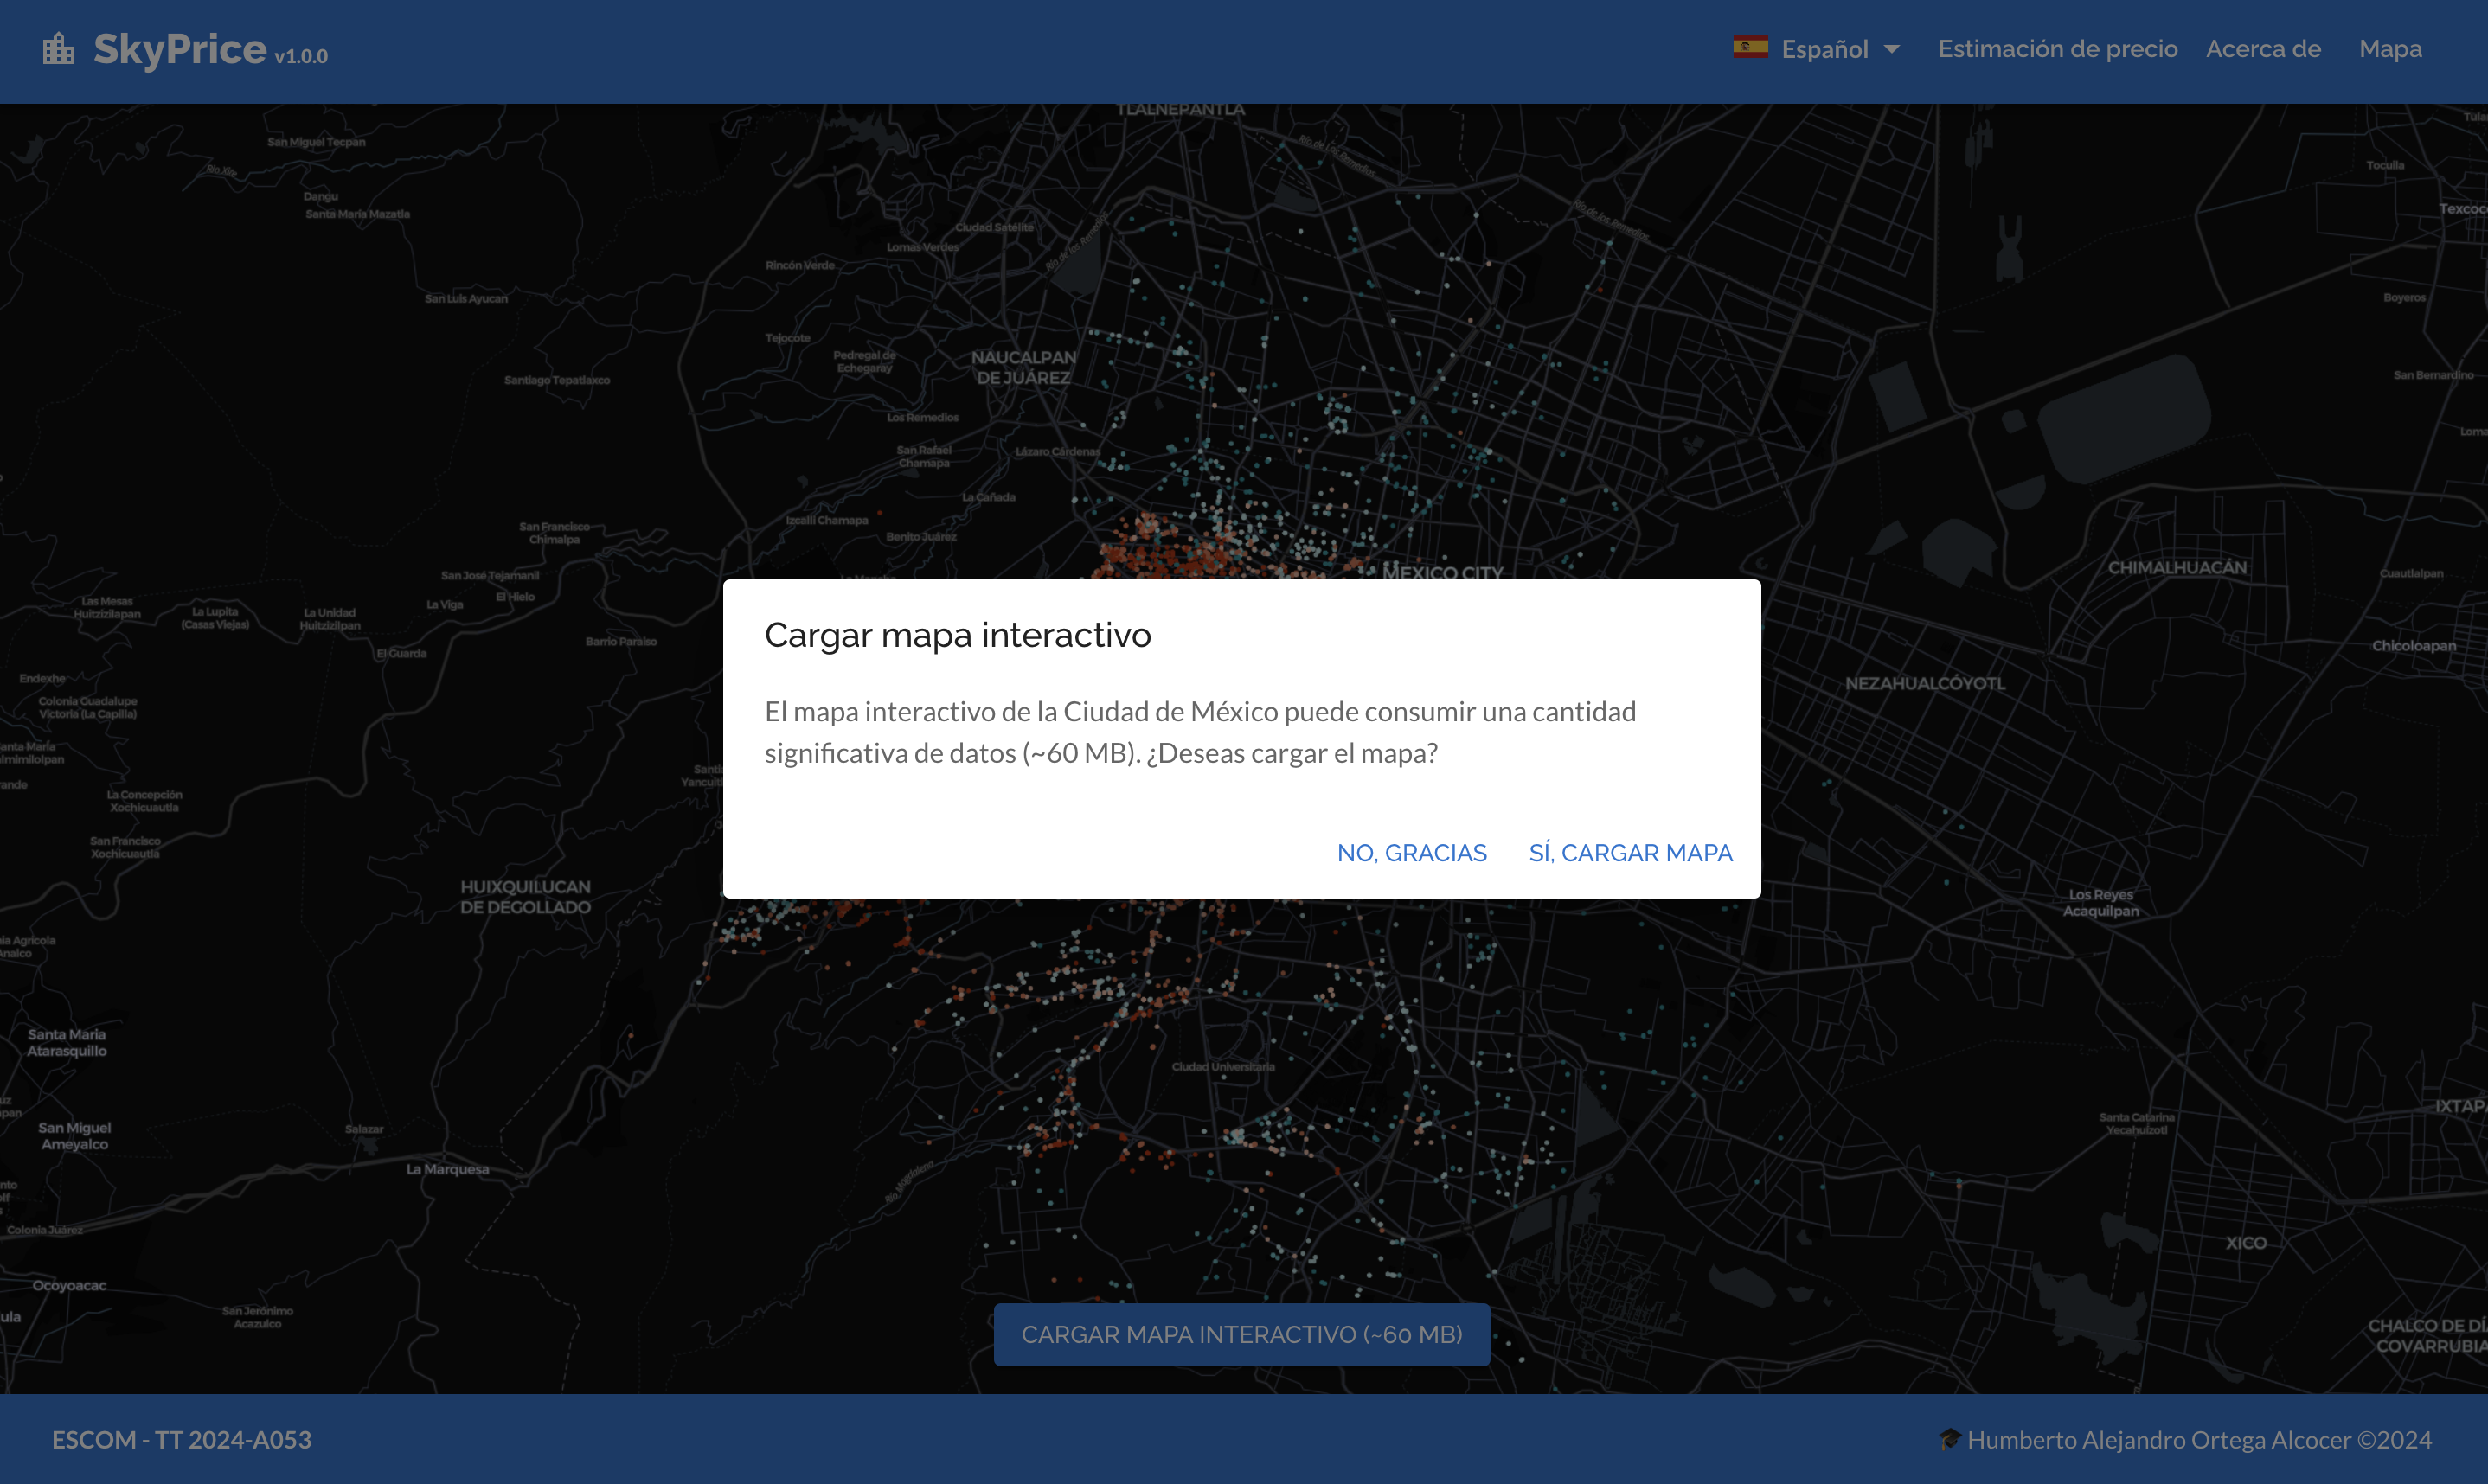
\includegraphics[width=0.8\textwidth]{imagenes/05-mapa-interactivo/aviso-consumo-recursos.png}
    \caption{Aviso de consumo de recursos}
    \label{fig:aviso-consumo-recursos}
\end{figure}

En caso de no querer continuar con la carga del mapa interactivo, el usuario
observará una imagen estática del mapa interactivo, como se muestra en la
figura \ref{fig:mapa-estatico}. Además se incluye un botón en la parte inferior
que permite al usuario en todo momento optar por sí cargar el mapa interactivo.

\begin{figure}[H]
    \centering
    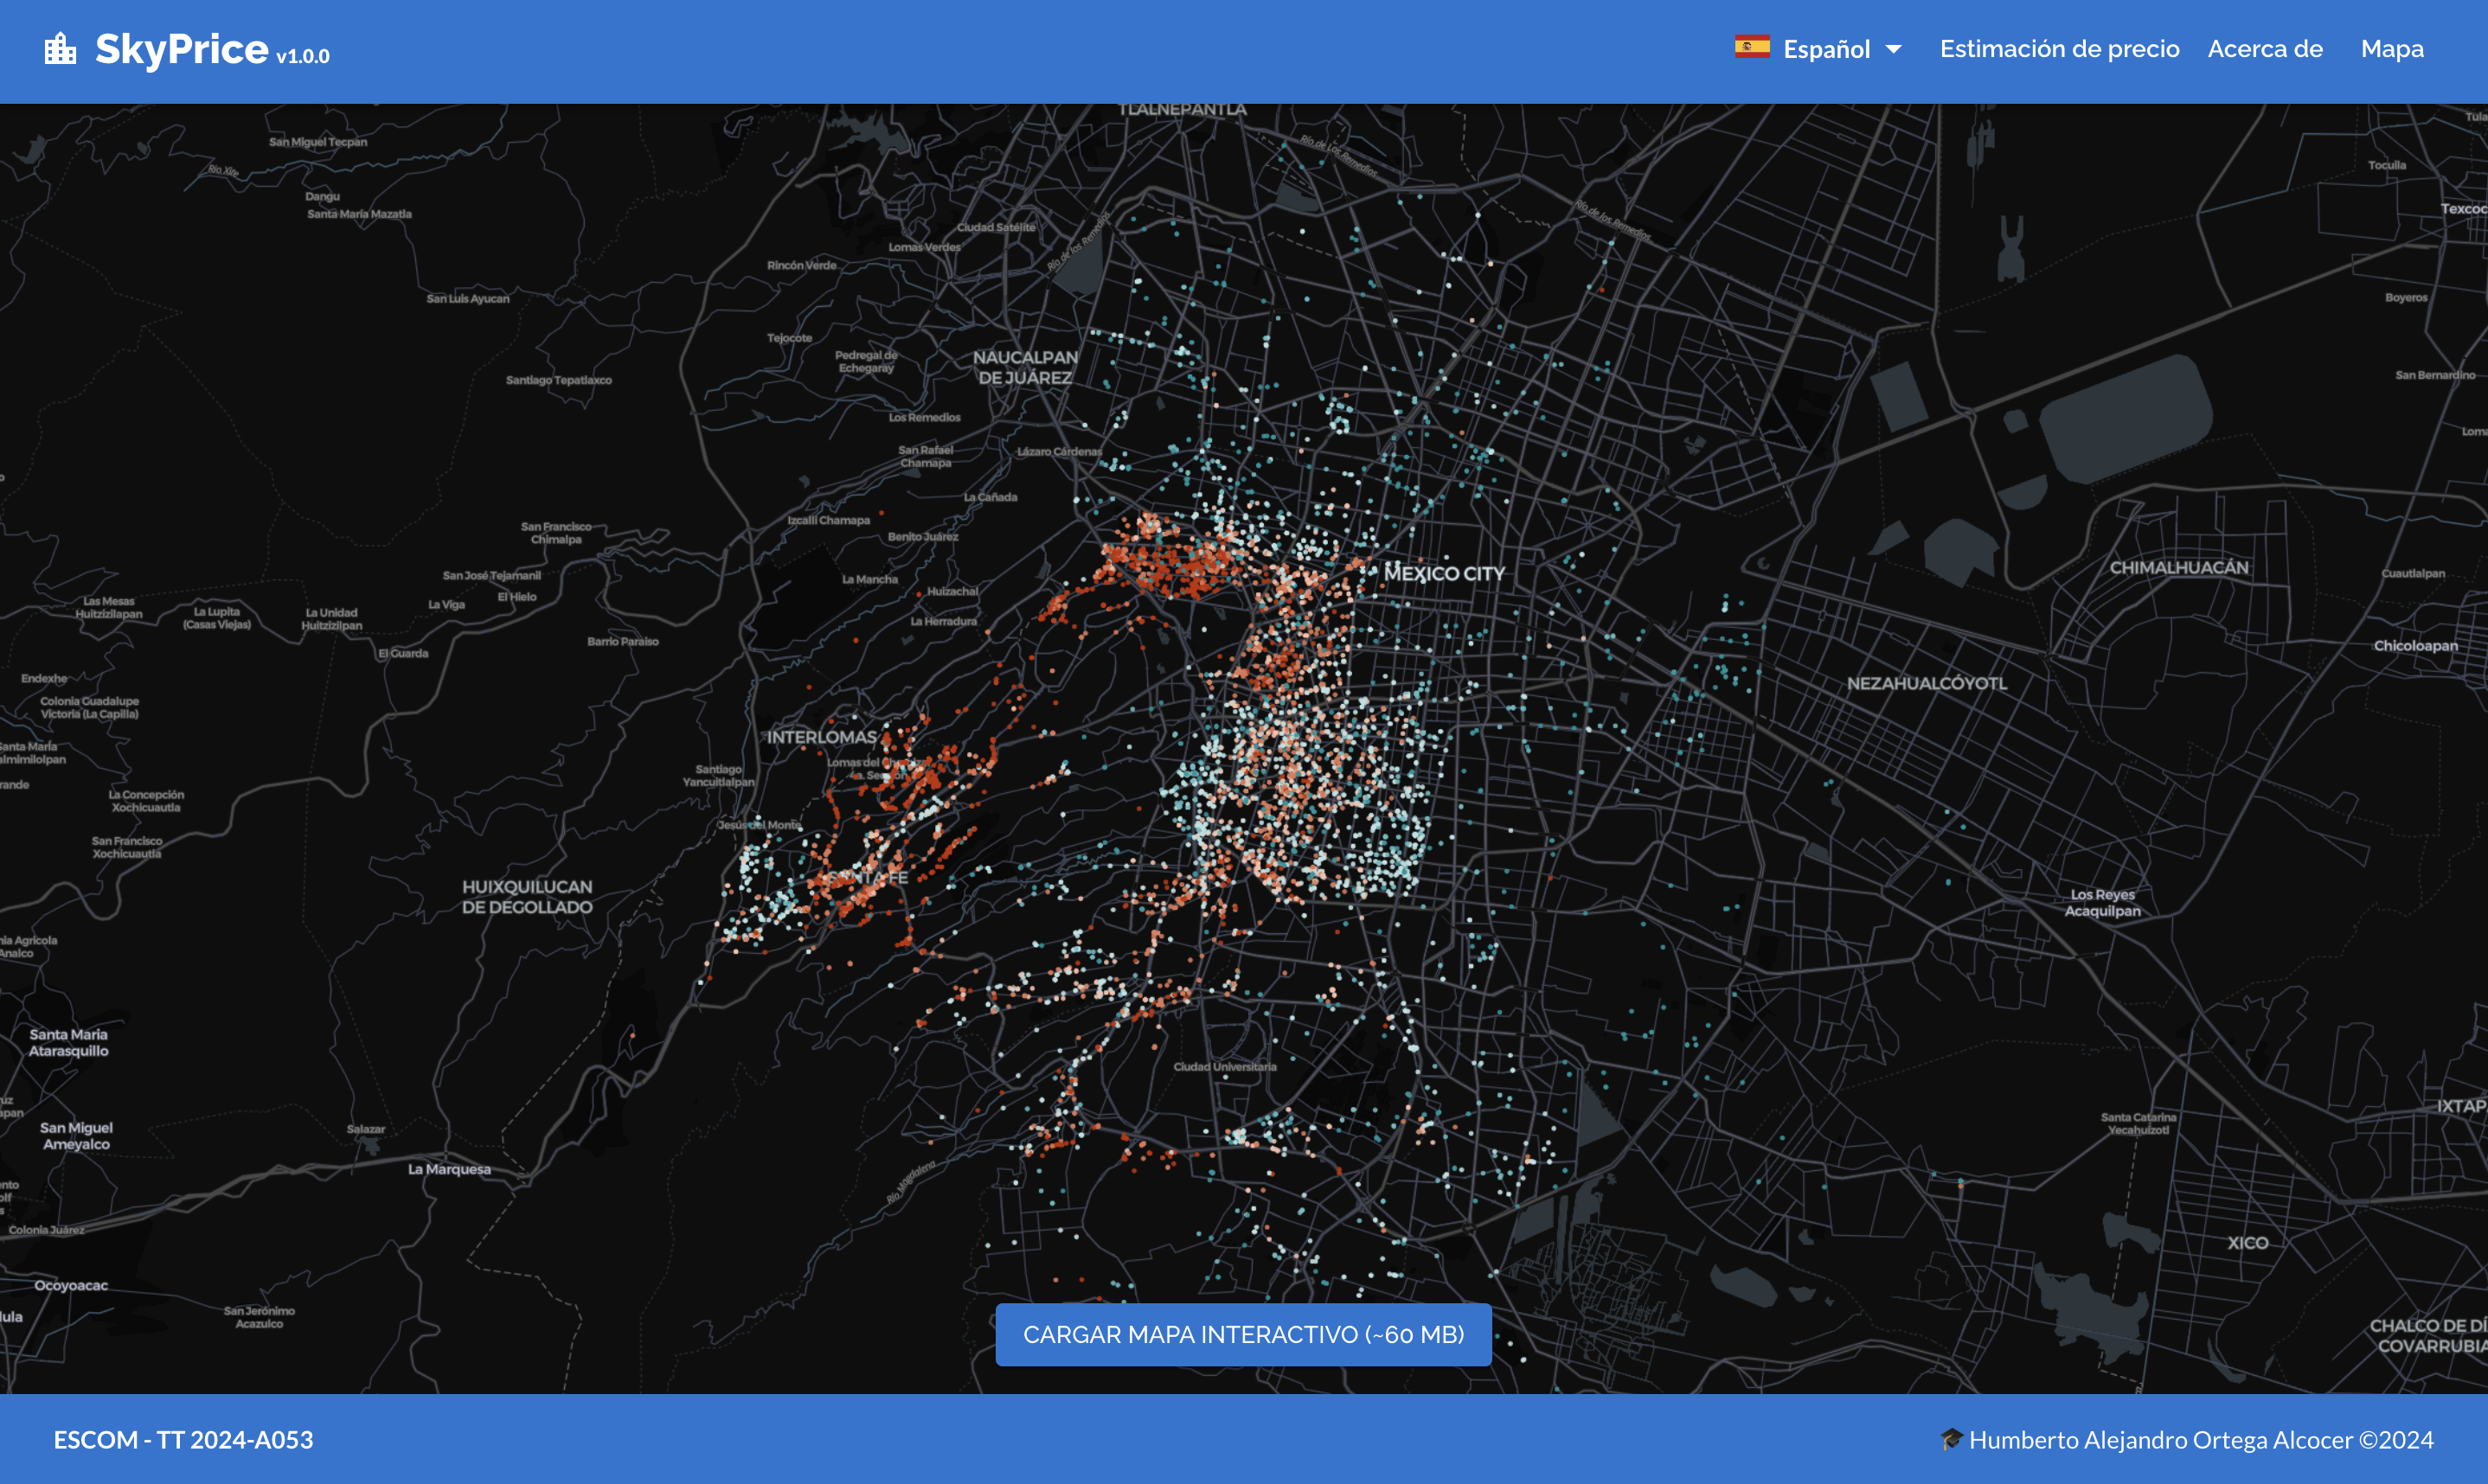
\includegraphics[width=0.8\textwidth]{imagenes/05-mapa-interactivo/mapa-estatico.png}
    \caption{Mapa estático}
    \label{fig:mapa-estatico}
\end{figure}

Si se decide continuar con la carga del mapa interactivo, se mostrará el mapa
interactivo en toda su funcionalidad. En la figura \ref{fig:mapa-interactivo}
se muestra el mapa interactivo.

\begin{figure}[H]
    \centering
    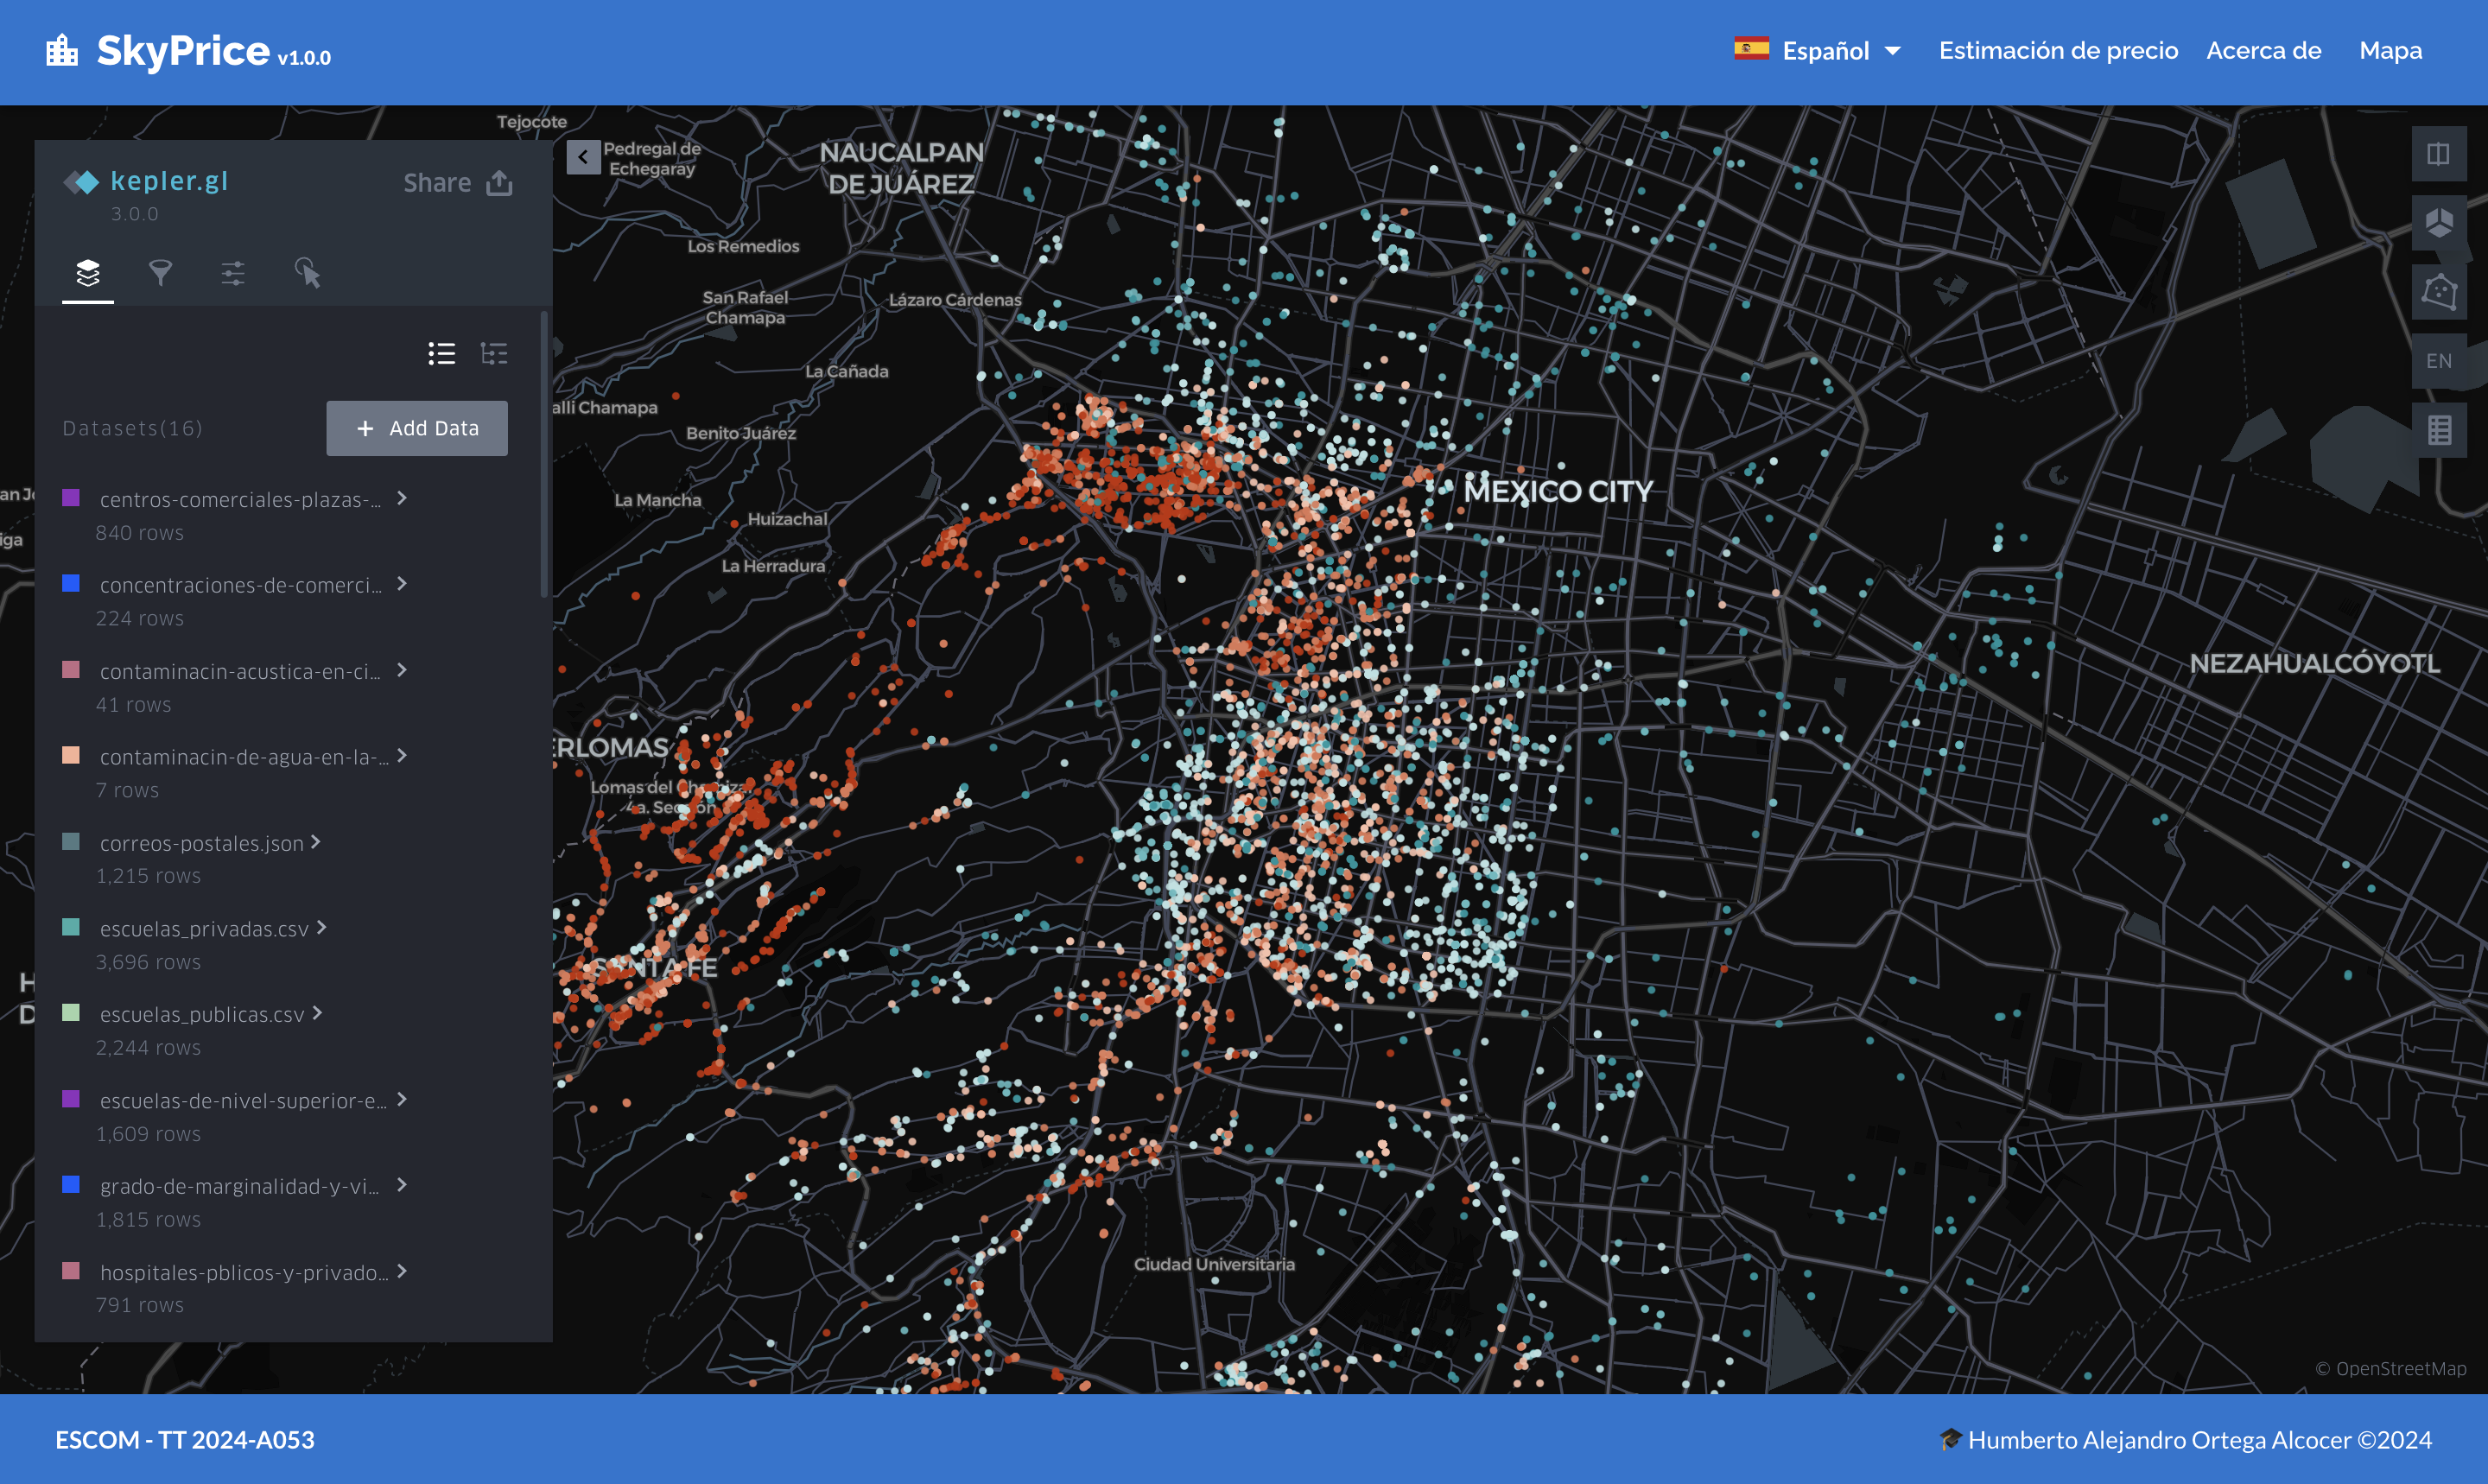
\includegraphics[width=0.8\textwidth]{imagenes/05-mapa-interactivo/mapa-interactivo.png}
    \caption{Mapa interactivo}
    \label{fig:mapa-interactivo}
\end{figure}

\section{Conjuntos de datos}
Con el fin de que el usuario pueda visualizar los datos de forma interactiva,
además de combinarlos con otras capas que podrían ser de interés, se han
integrado múltiples conjuntos de datos geoespaciales en el mapa interactivo.

\subsection{Anuncios de departamentos}
Los datos iniciales que se han integrado en el mapa interactivo son los
anuncios de departamentos utilizados en el entrenamiento de los modelos de
aprendizaje automático. La capa muestra la ubicación de los anuncios y utiliza
un gradiente de color para representar el precio de los departamentos.

En la figura \ref{fig:anuncios-departamentos} se muestra la capa de anuncios de
departamentos.

\begin{figure}[H]
    \centering
    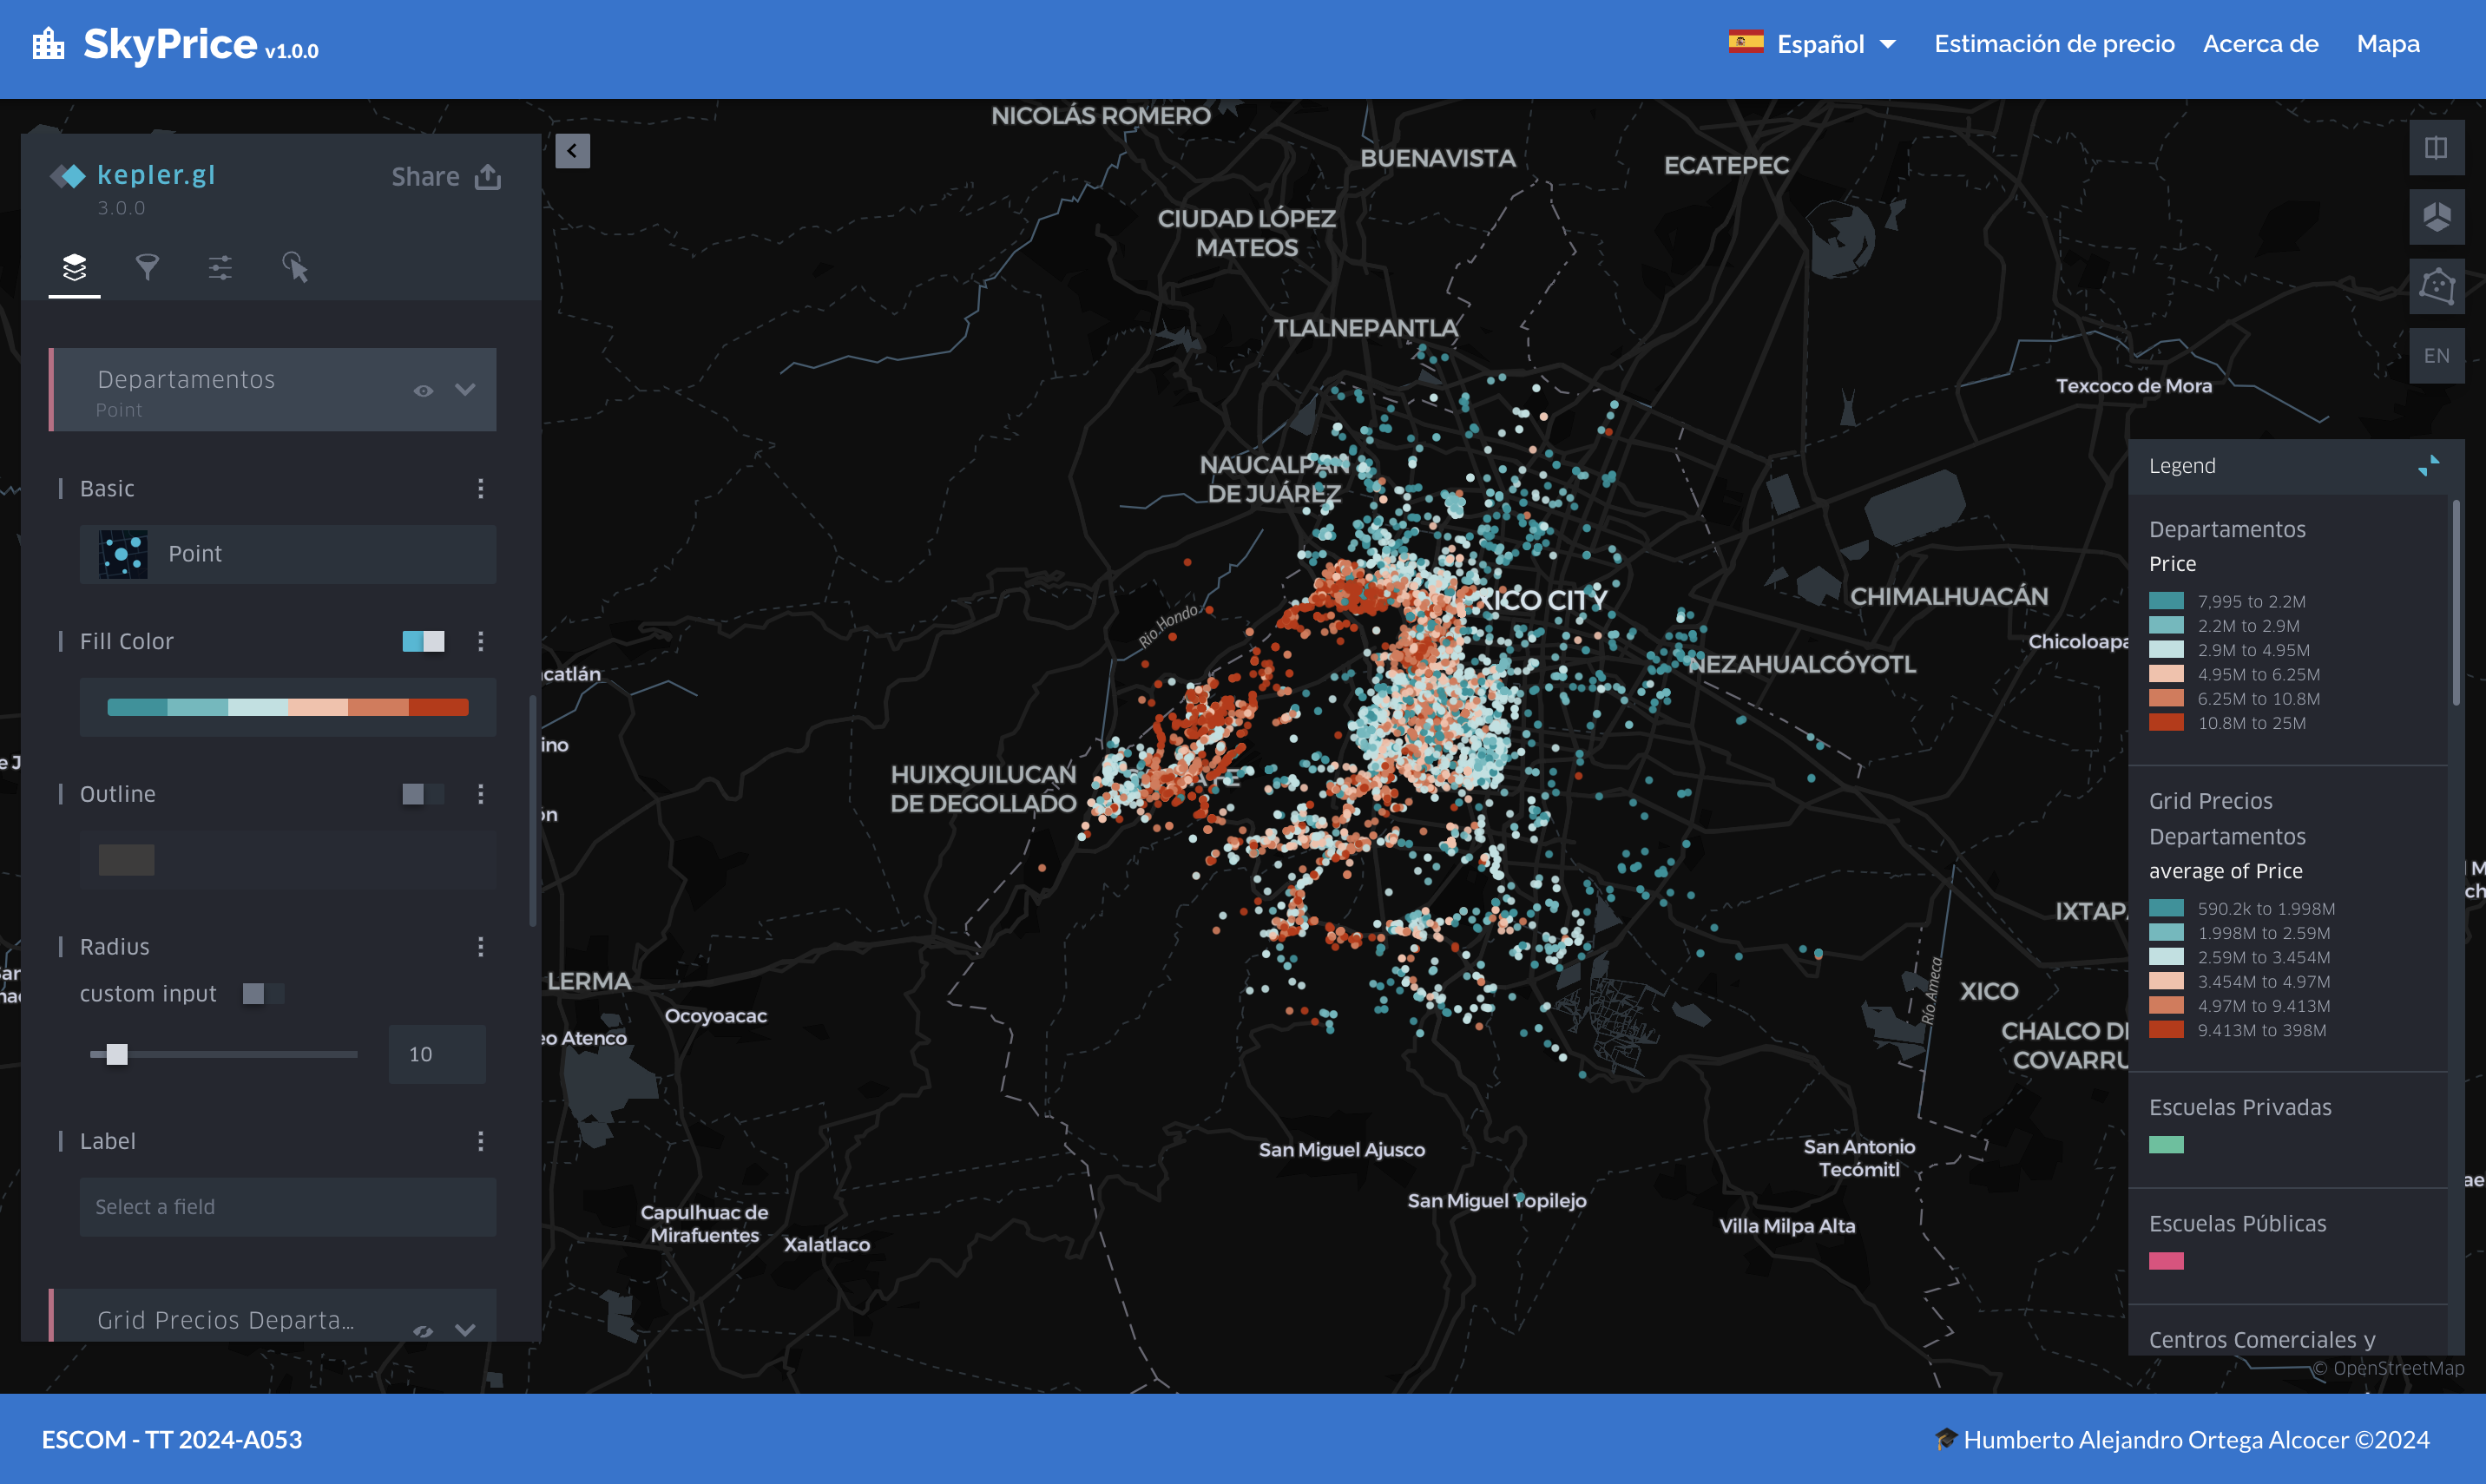
\includegraphics[width=0.8\textwidth]{imagenes/05-mapa-interactivo/anuncios-departamentos.png}
    \caption{Anuncios de departamentos}
    \label{fig:anuncios-departamentos}
\end{figure}

\subsection{Grid de precios de departamentos}
Además de los anuncios de departamentos, se ha integrado un grid de precios de
departamentos. Este grid divide la Ciudad de México en celdas de 1 kilómetro cuadrado
calcula el precio promedio de los departamentos en cada celda.

En la figura \ref{fig:grid-precios-departamentos} se muestra la capa de grid de
precios de departamentos.

\begin{figure}[H]
    \centering
    \includegraphics[width=0.8\textwidth]{imagenes/05-mapa-interactivo/grid-precios-departamentos.png}
    \caption{Grid de precios de departamentos}
    \label{fig:grid-precios-departamentos}
\end{figure}

\subsection{Escuelas privadas}
Esta capa contiene la ubicación de las escuelas privadas en la Ciudad de México,
desde Kínder hasta Secundaria. En la figura \ref{fig:escuelas-privadas} se muestra
la capa de escuelas privadas.

\begin{figure}[H]
    \centering
    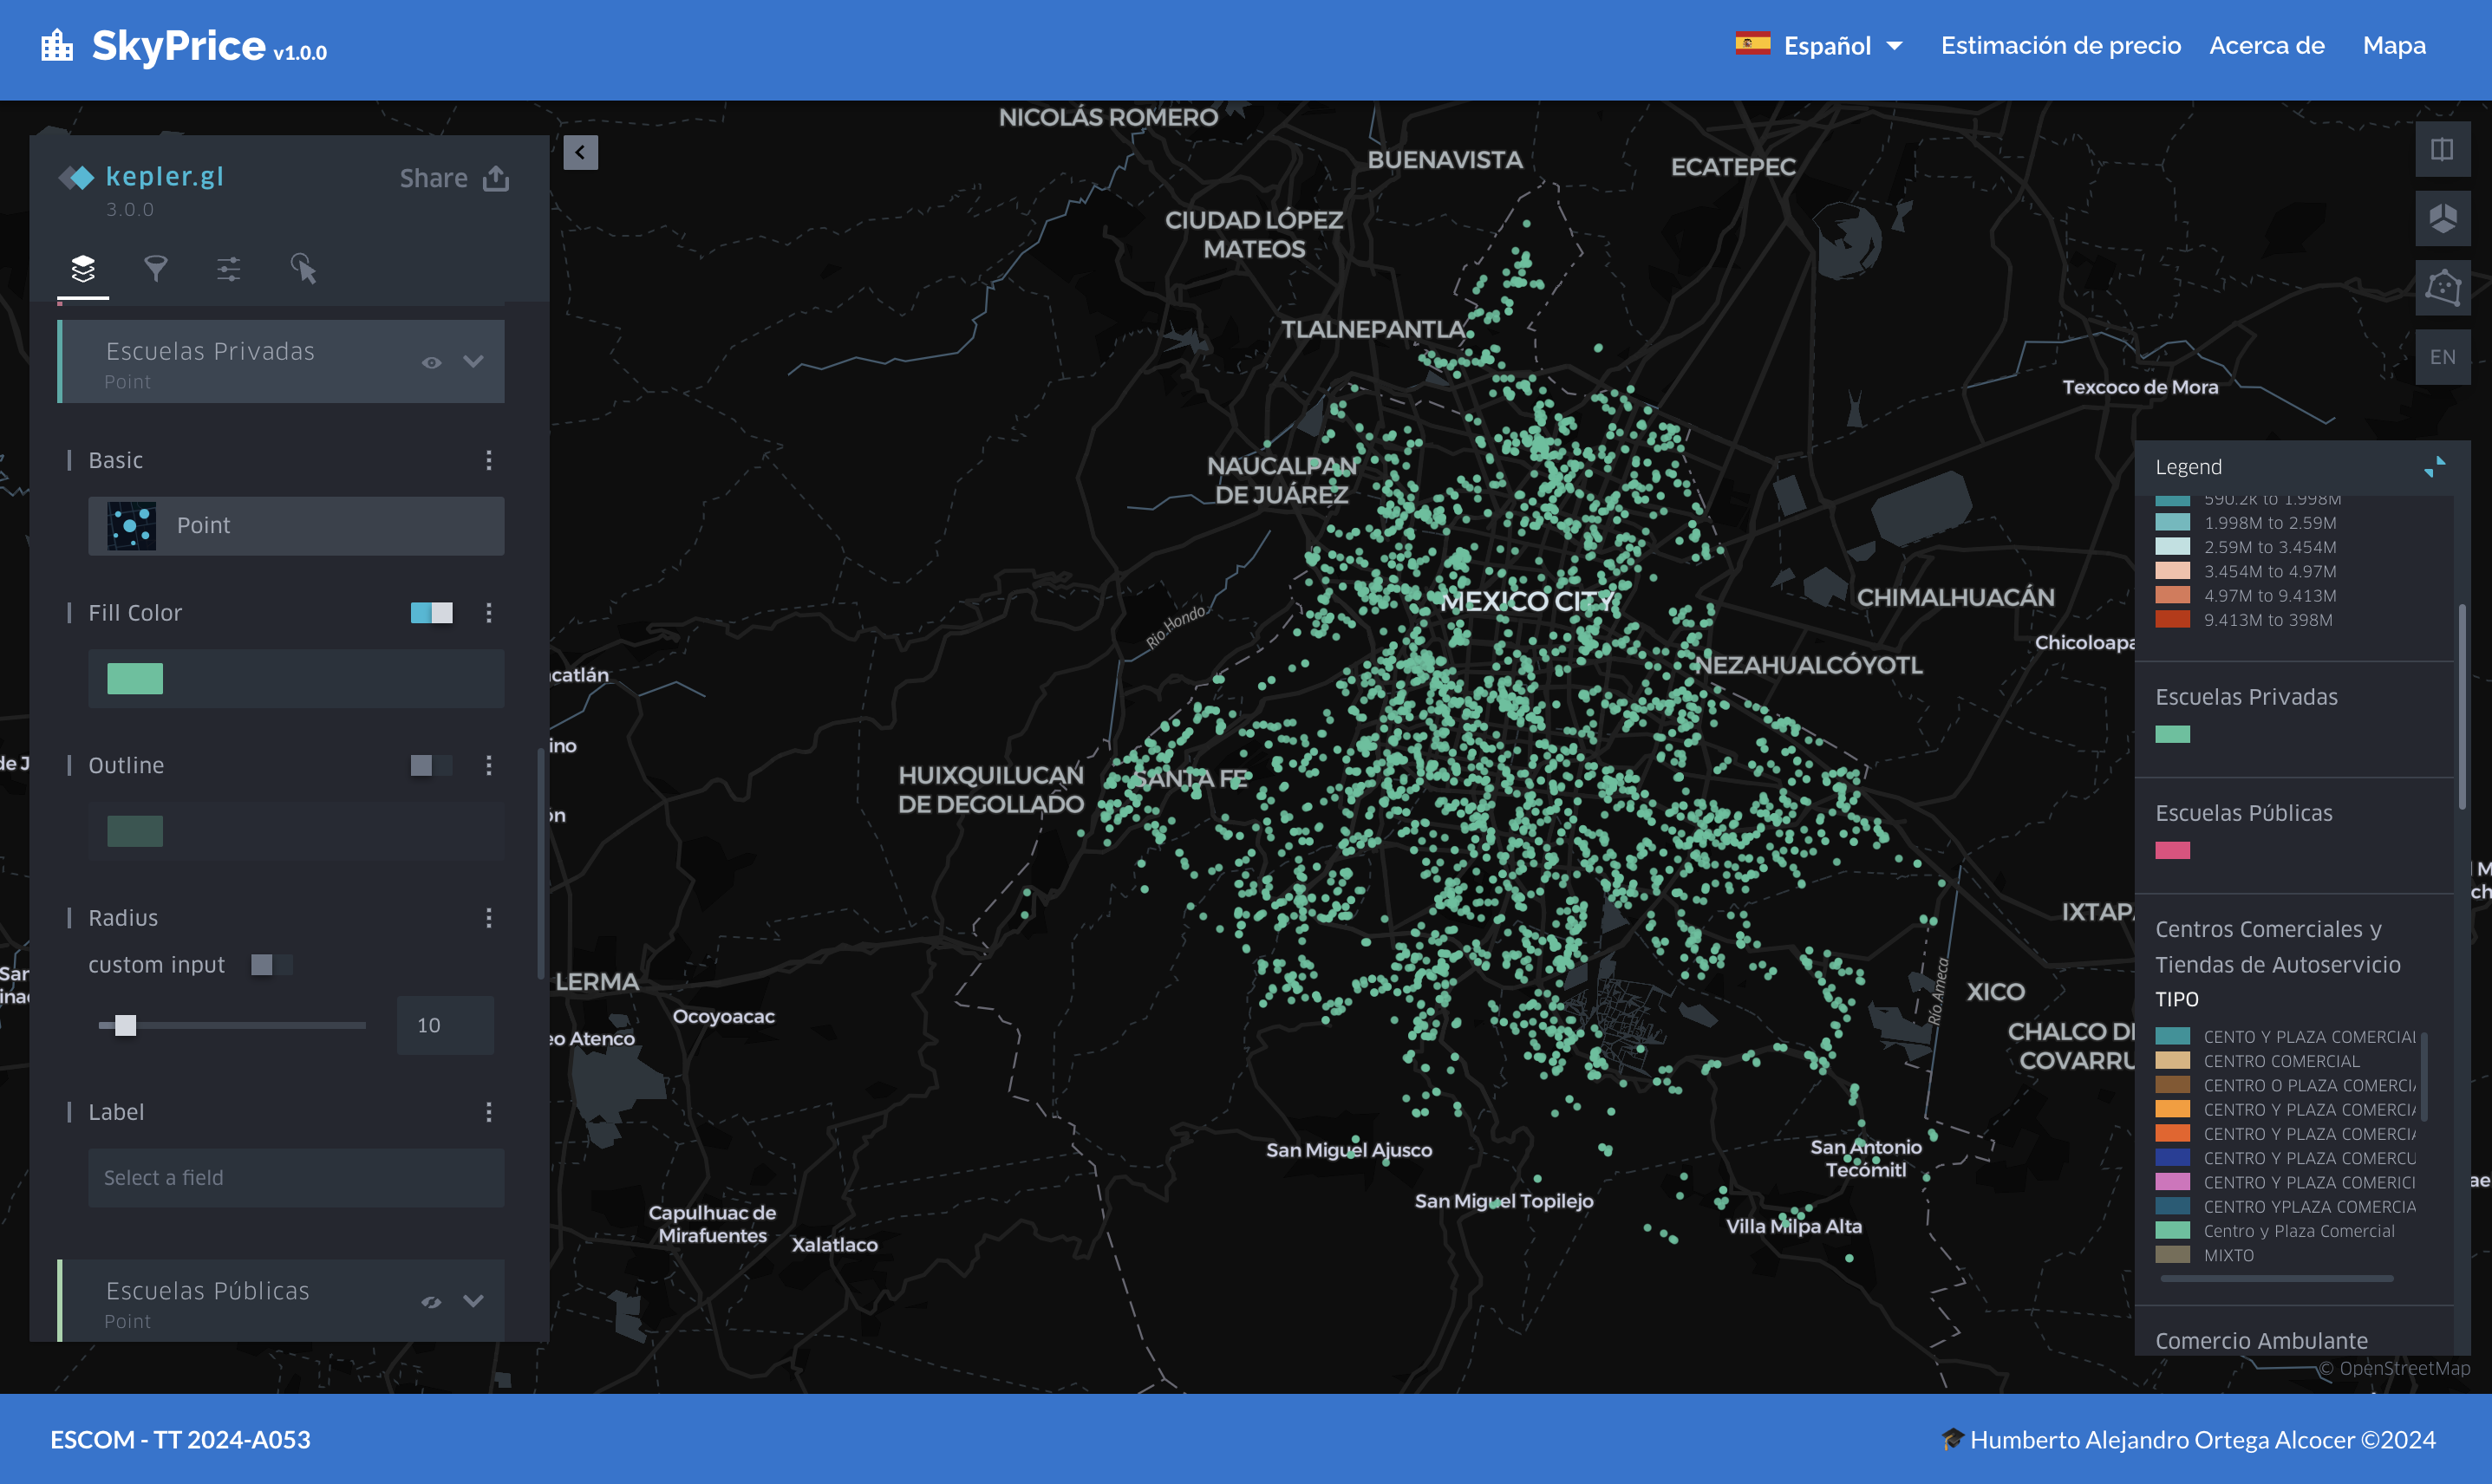
\includegraphics[width=0.8\textwidth]{imagenes/05-mapa-interactivo/escuelas-privadas.png}
    \caption{Escuelas privadas}
    \label{fig:escuelas-privadas}
\end{figure}

\subsection{Escuelas públicas}
Esta capa contiene la ubicación de las escuelas públicas en la Ciudad de México,
desde Kínder hasta Secundaria. En la figura \ref{fig:escuelas-publicas} se muestra
la capa de escuelas públicas.

\begin{figure}[H]
    \centering
    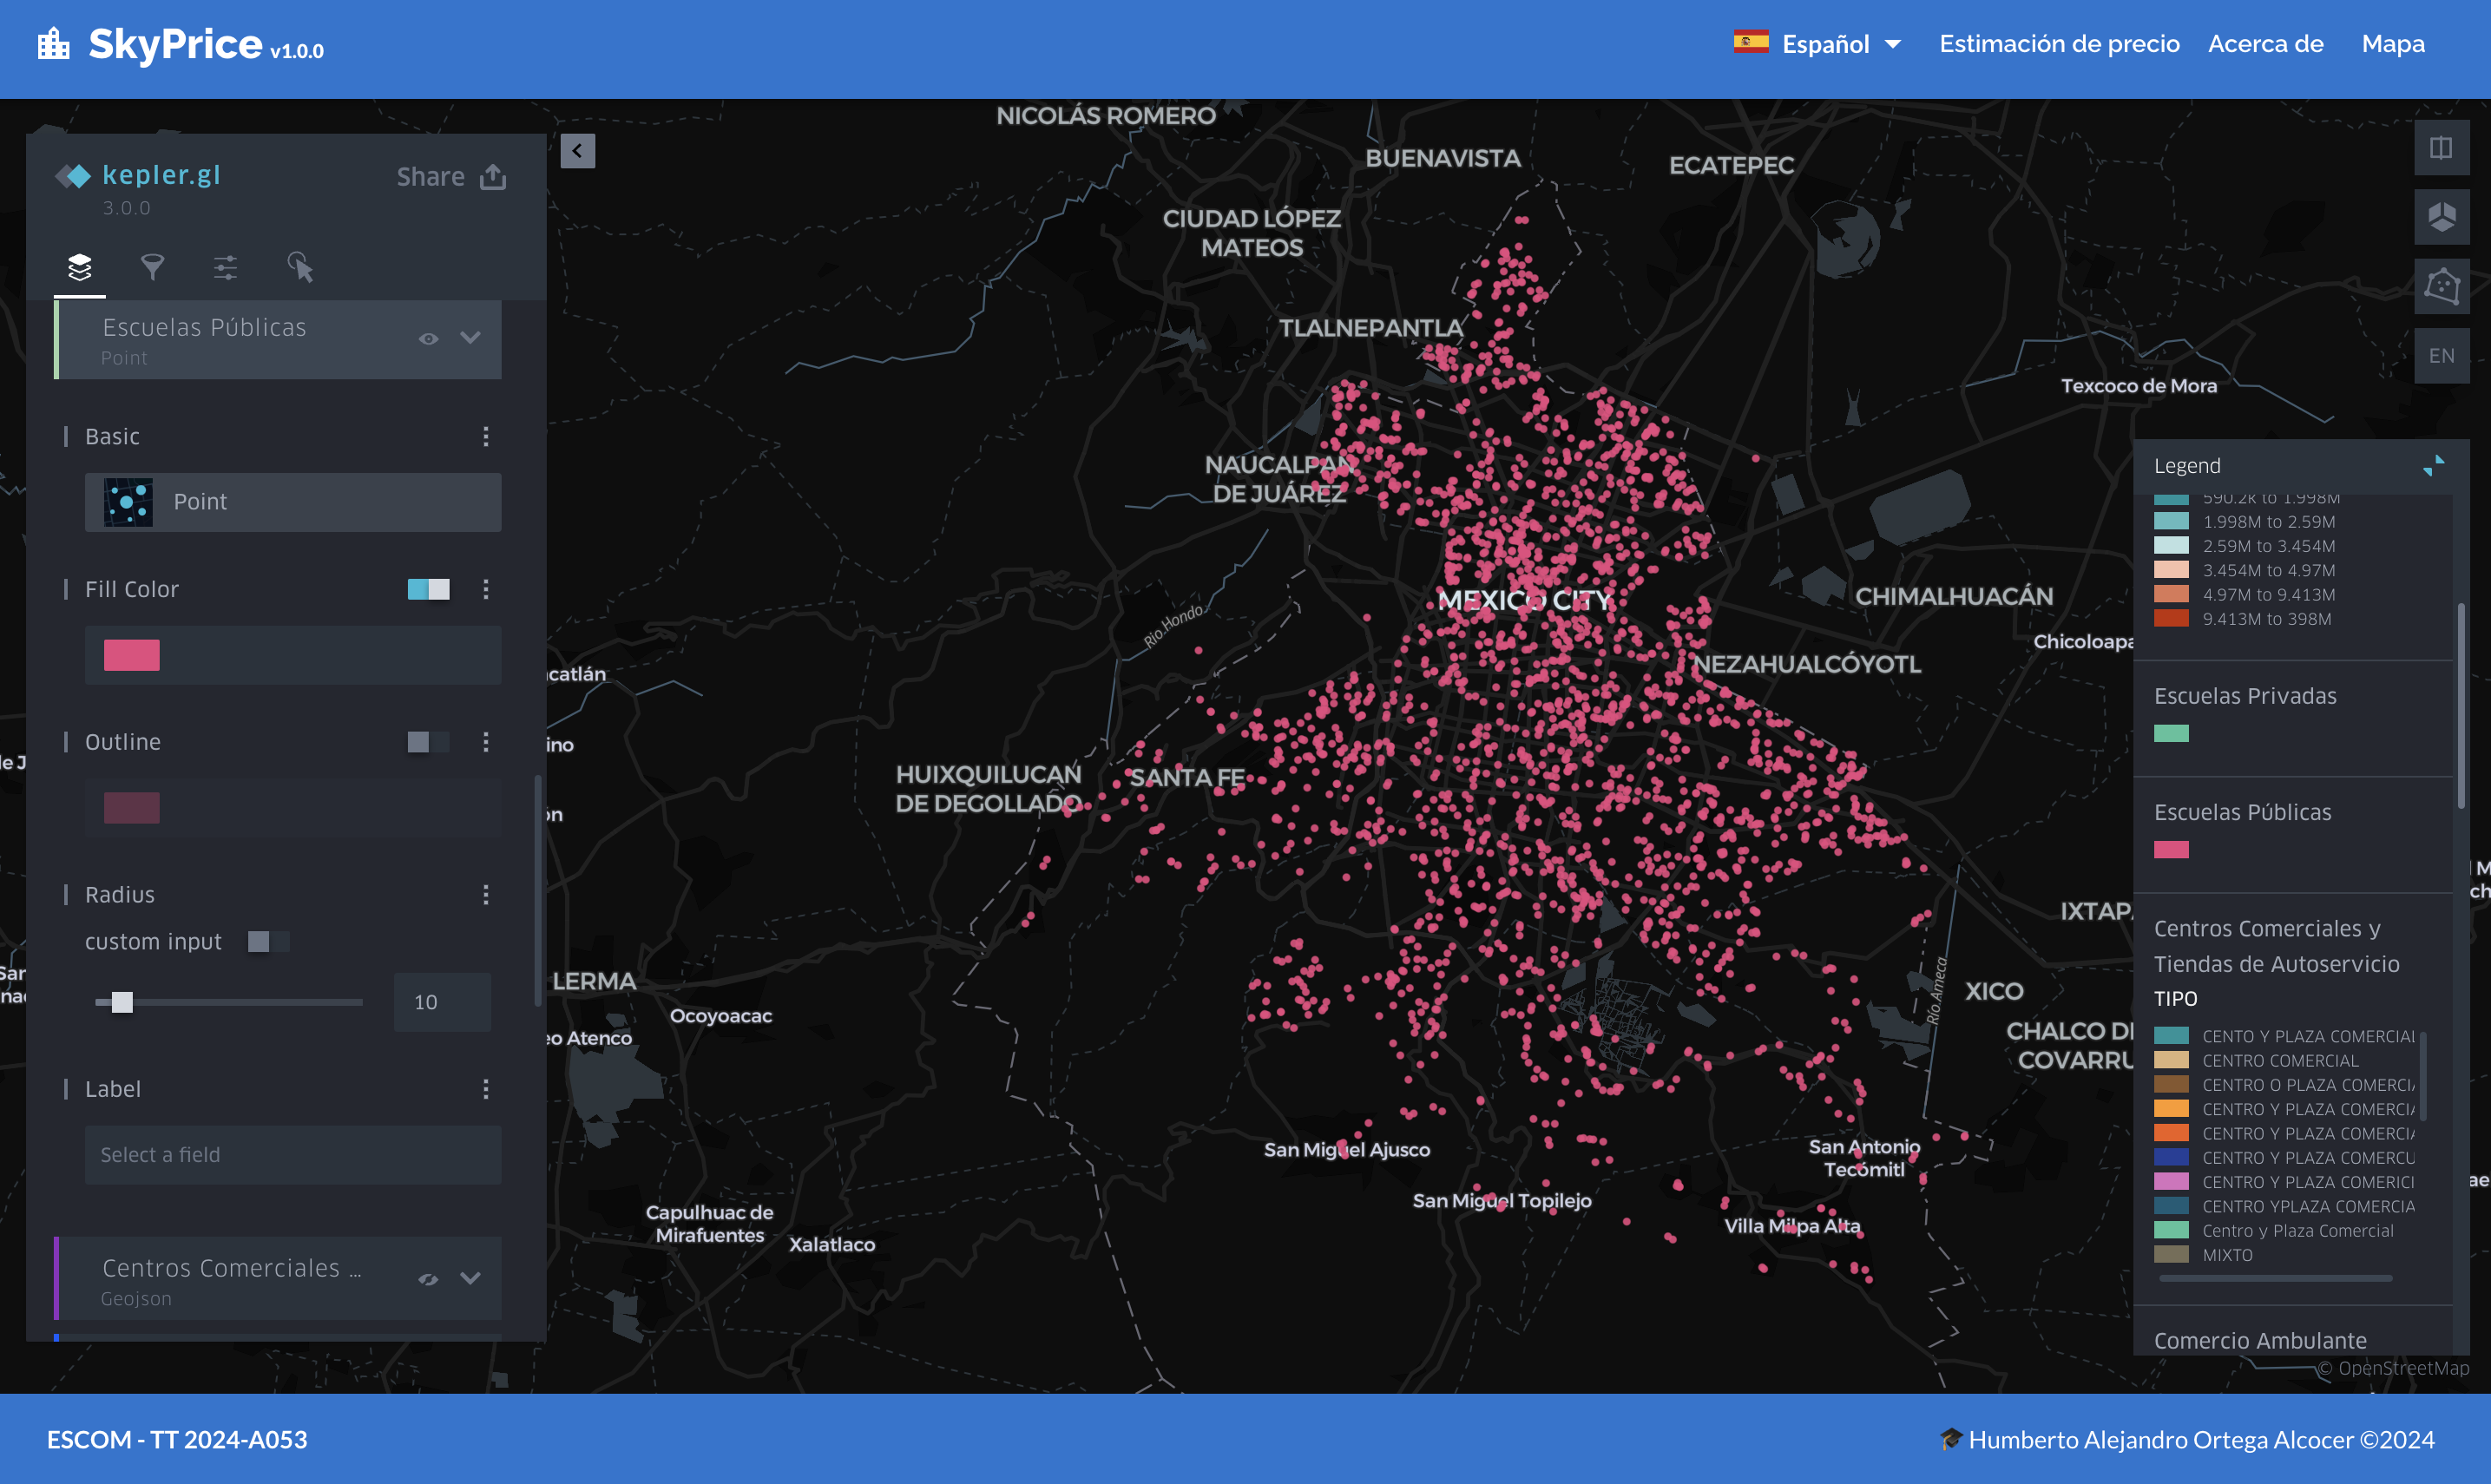
\includegraphics[width=0.8\textwidth]{imagenes/05-mapa-interactivo/escuelas-publicas.png}
    \caption{Escuelas públicas}
    \label{fig:escuelas-publicas}
\end{figure}

\subsection{Centros Comerciales}
Esta capa contiene la ubicación de centros comerciales, tiendas de autoservicio y
plazas comerciales en la Ciudad de México. En la figura \ref{fig:centros-comerciales}
se muestra la capa de centros comerciales.

\begin{figure}[H]
    \centering
    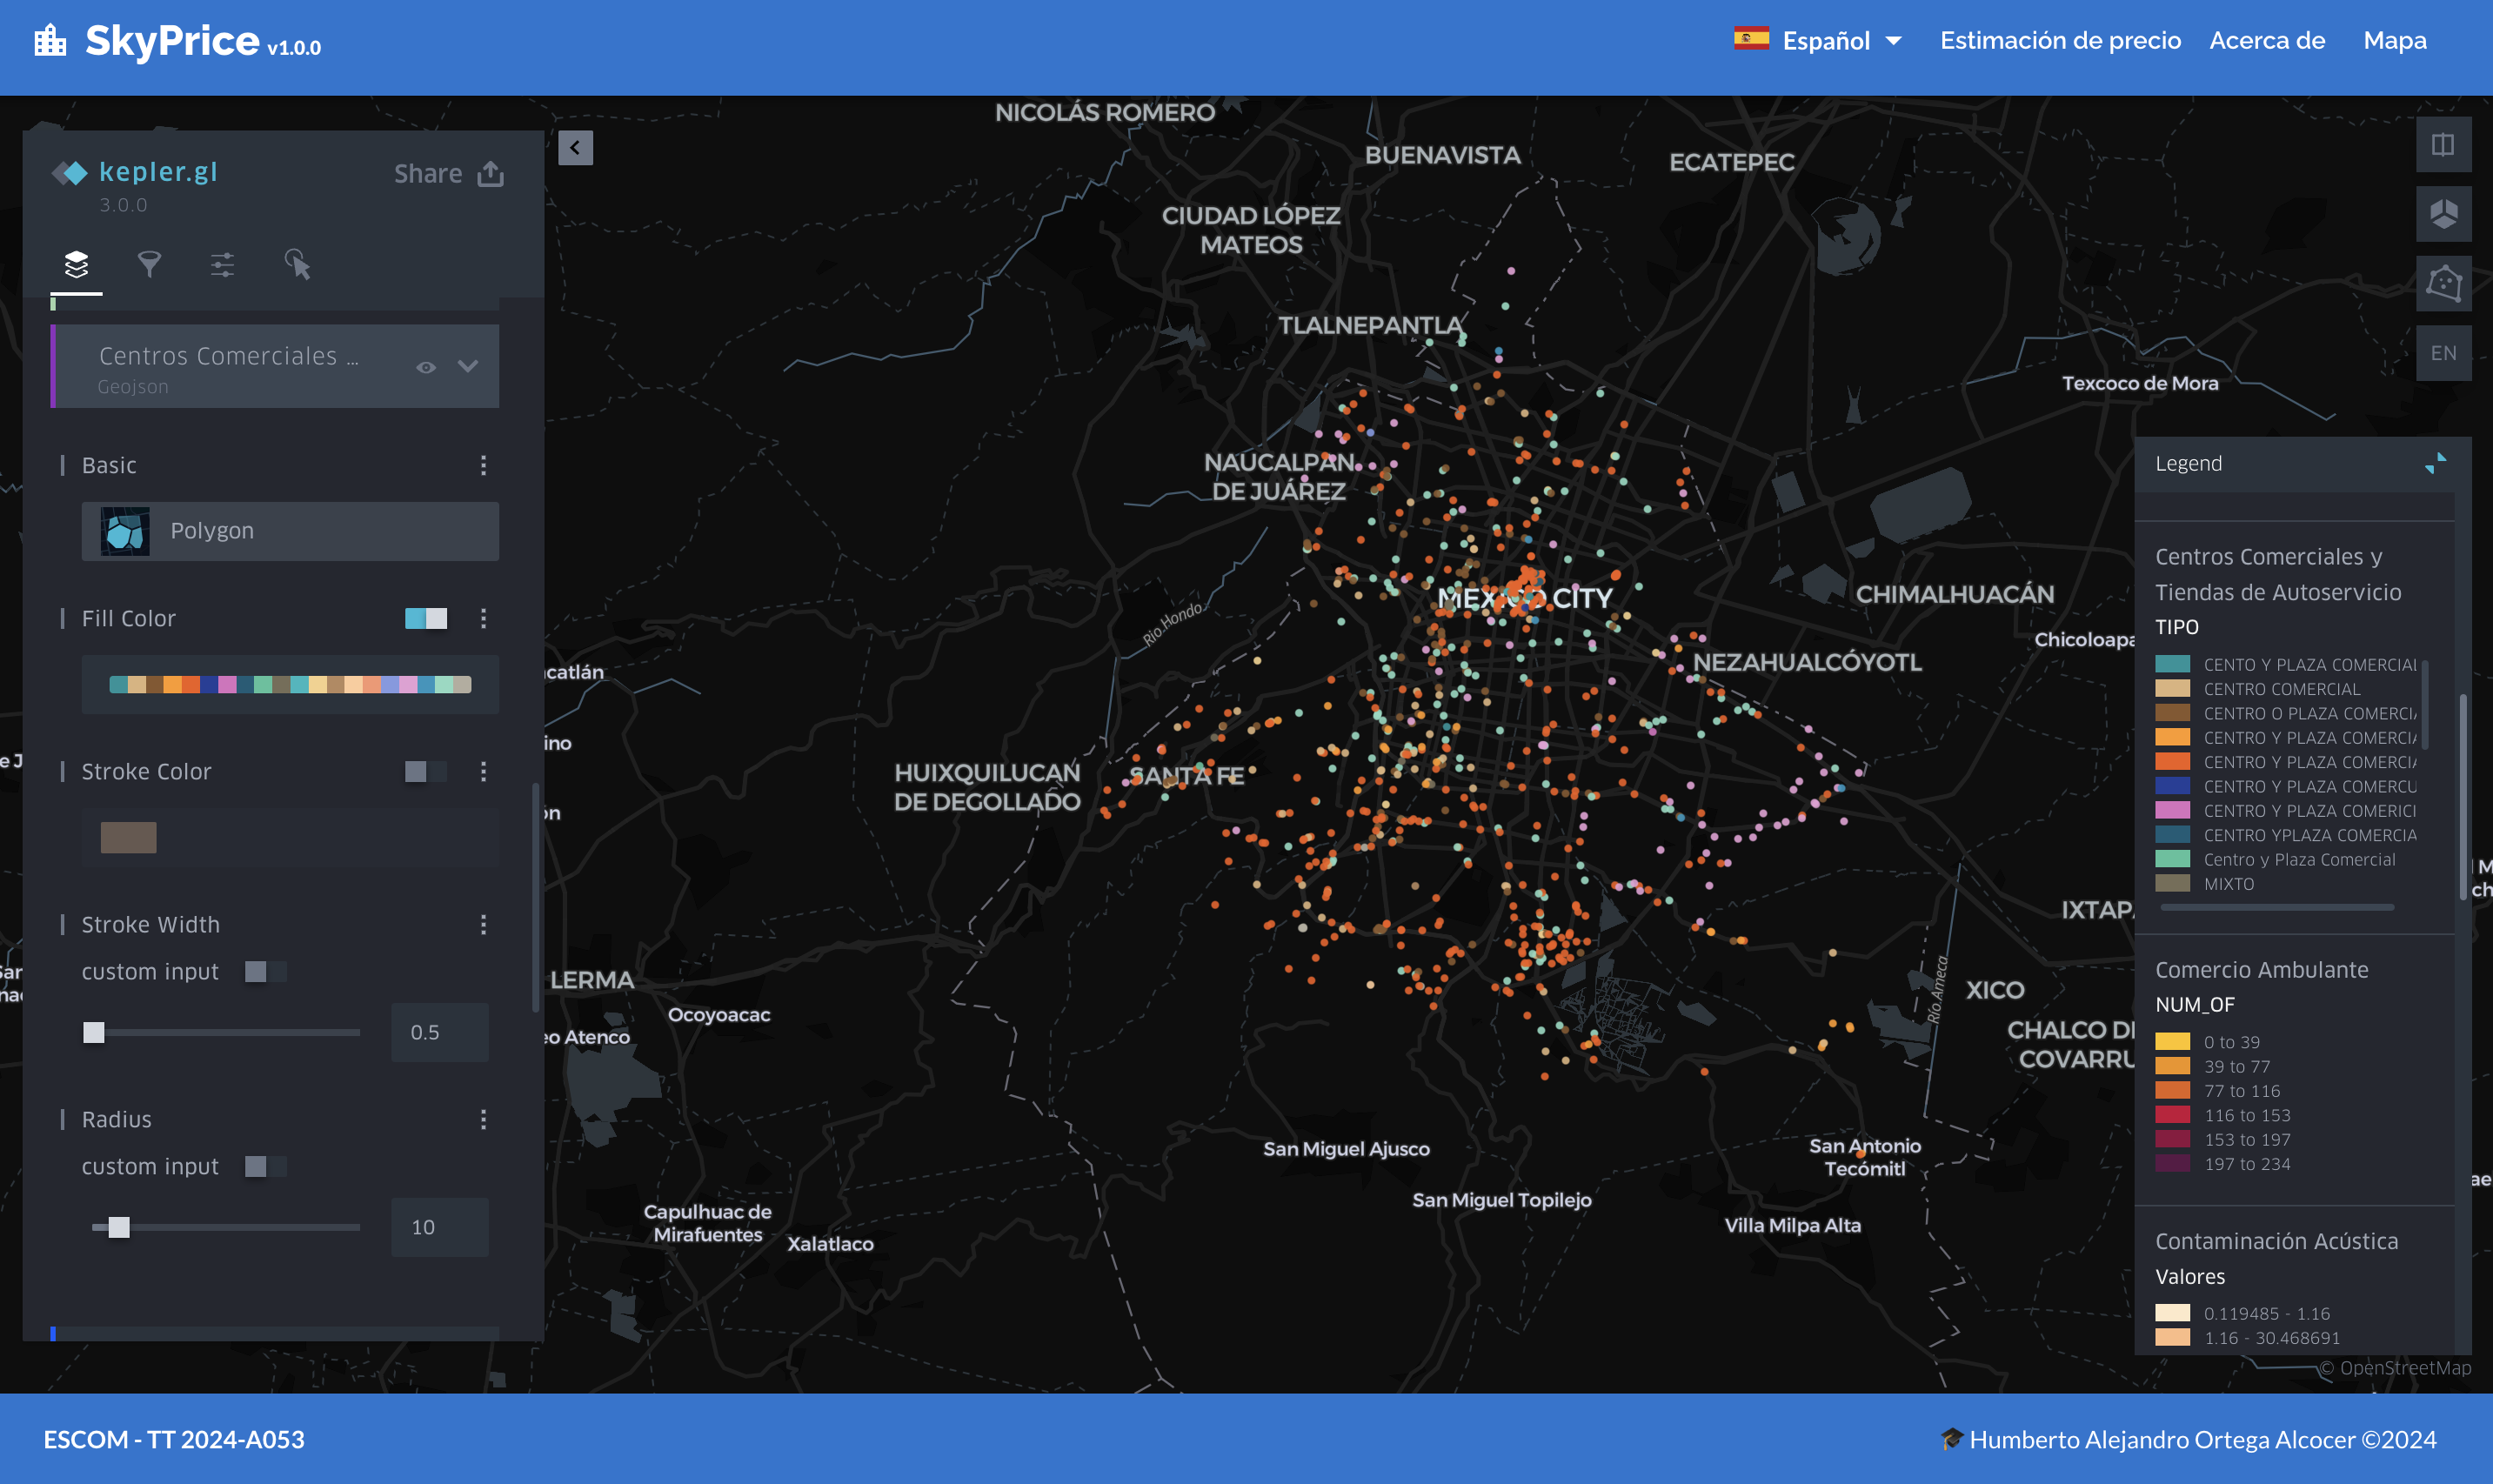
\includegraphics[width=0.8\textwidth]{imagenes/05-mapa-interactivo/centros-comerciales.png}
    \caption{Centros comerciales}
    \label{fig:centros-comerciales}
\end{figure}

\subsection{Comercio ambulante}
Esta capa contiene la ubicación de comercio ambulante en la Ciudad de México. En
la figura \ref{fig:comercio-ambulante} se muestra la capa de comercio ambulante.

\begin{figure}[H]
    \centering
    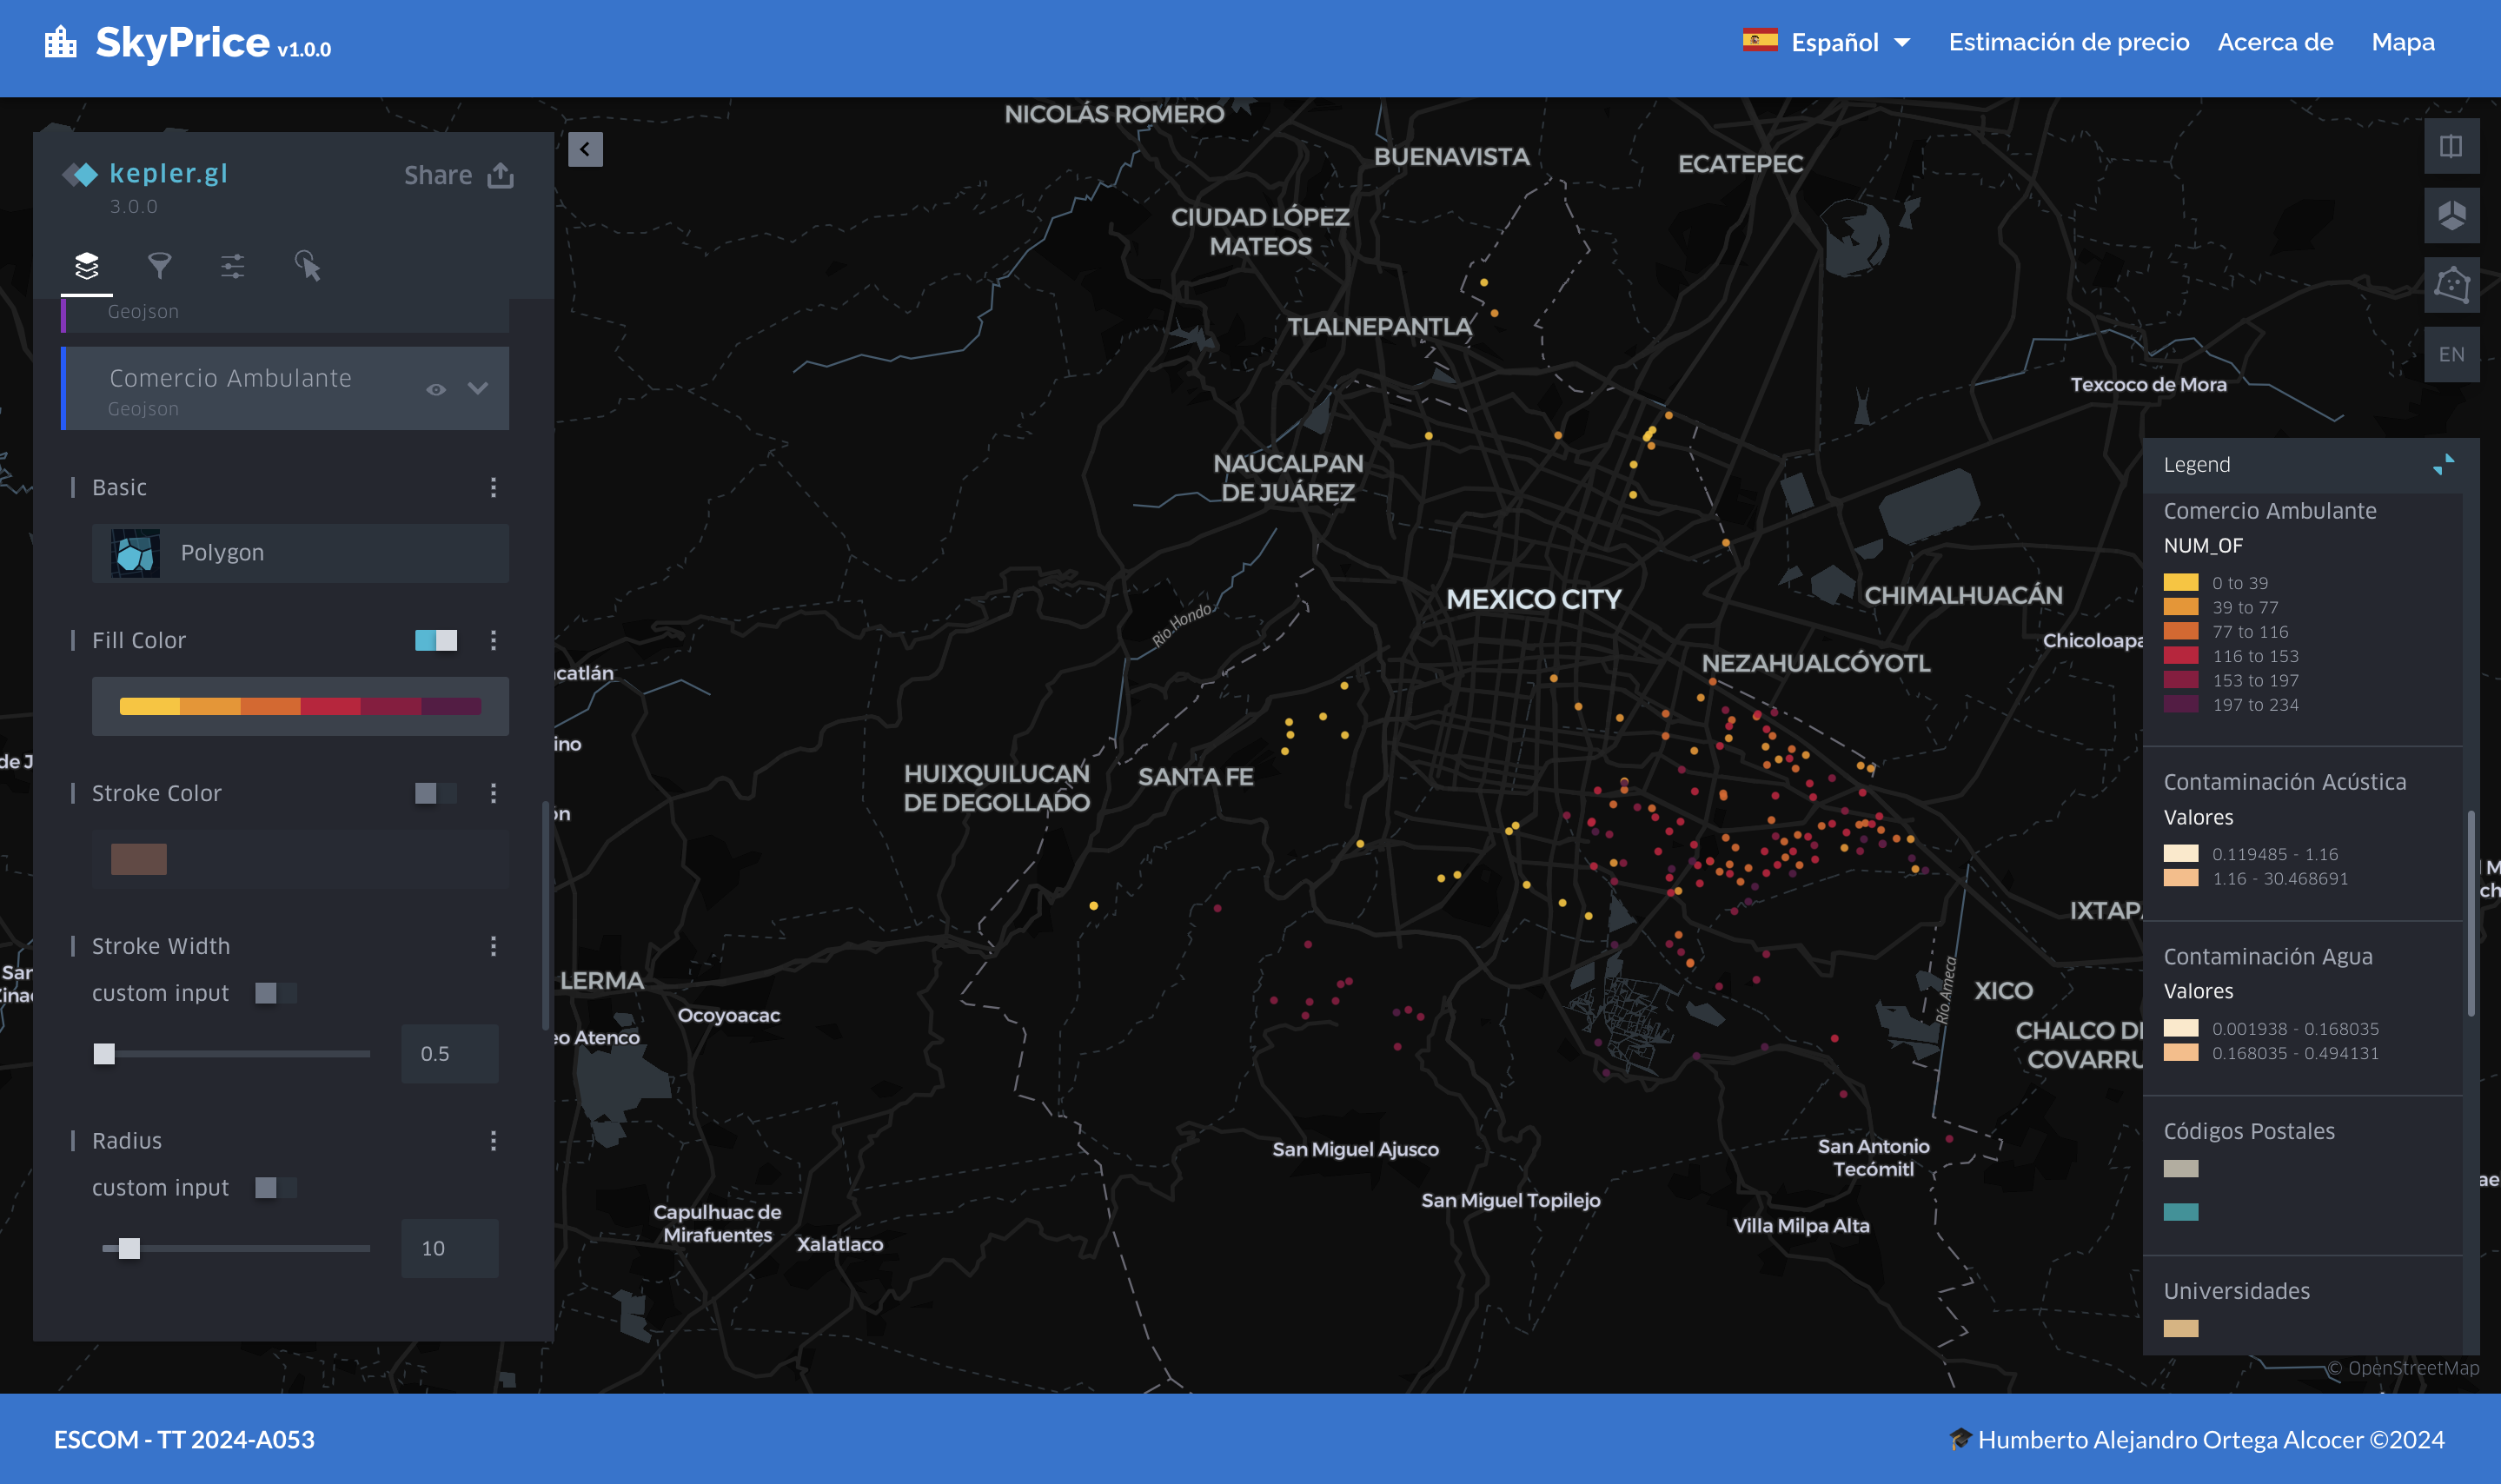
\includegraphics[width=0.8\textwidth]{imagenes/05-mapa-interactivo/comercio-ambulante.png}
    \caption{Comercio ambulante}
    \label{fig:comercio-ambulante}
\end{figure}

\subsection{Contaminación acústica}
Esta capa contiene los polígonos con los niveles de contaminación acústica en la
Ciudad de México. En la figura \ref{fig:contaminacion-acustica} se muestra la capa
de contaminación acústica.

\begin{figure}[H]
    \centering
    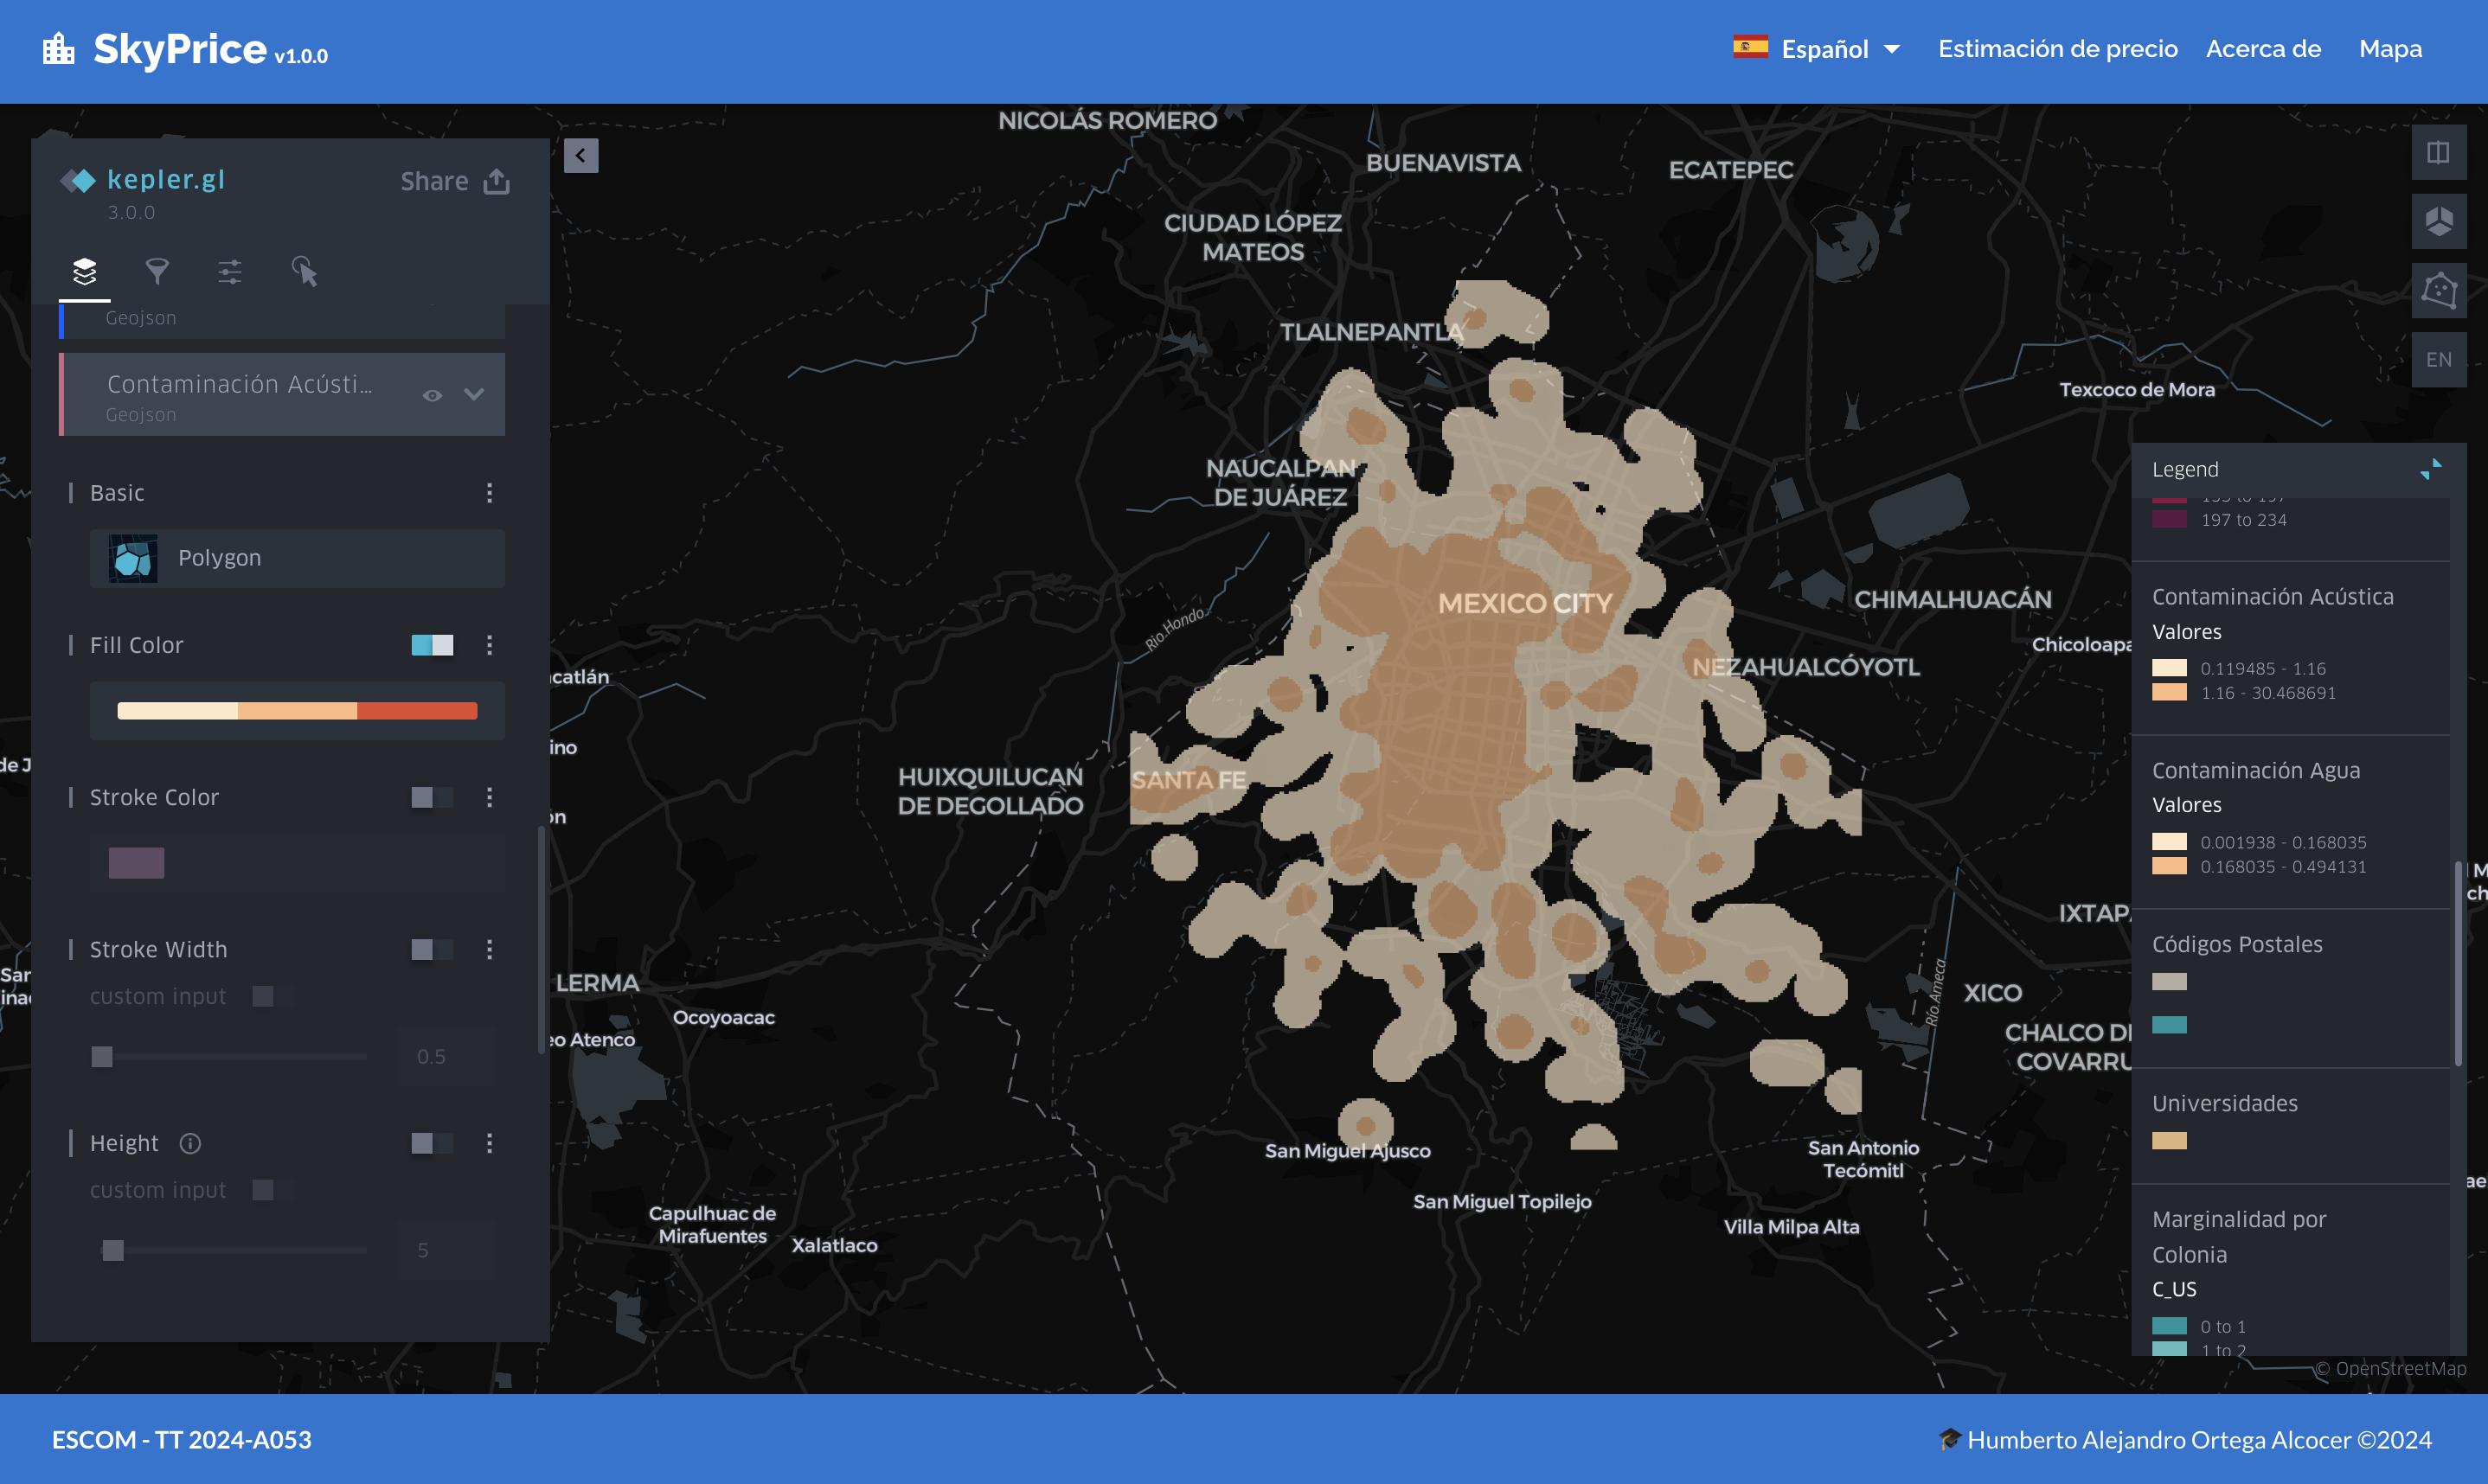
\includegraphics[width=0.8\textwidth]{imagenes/05-mapa-interactivo/contaminacion-acustica.png}
    \caption{Contaminación acústica}
    \label{fig:contaminacion-acustica}
\end{figure}

\subsection{Contaminación del agua}
Esta capa contiene los polígonos con los niveles de contaminación del agua en la
Ciudad de México. En la figura \ref{fig:contaminacion-agua} se muestra la capa de
contaminación del agua.

\begin{figure}[H]
    \centering
    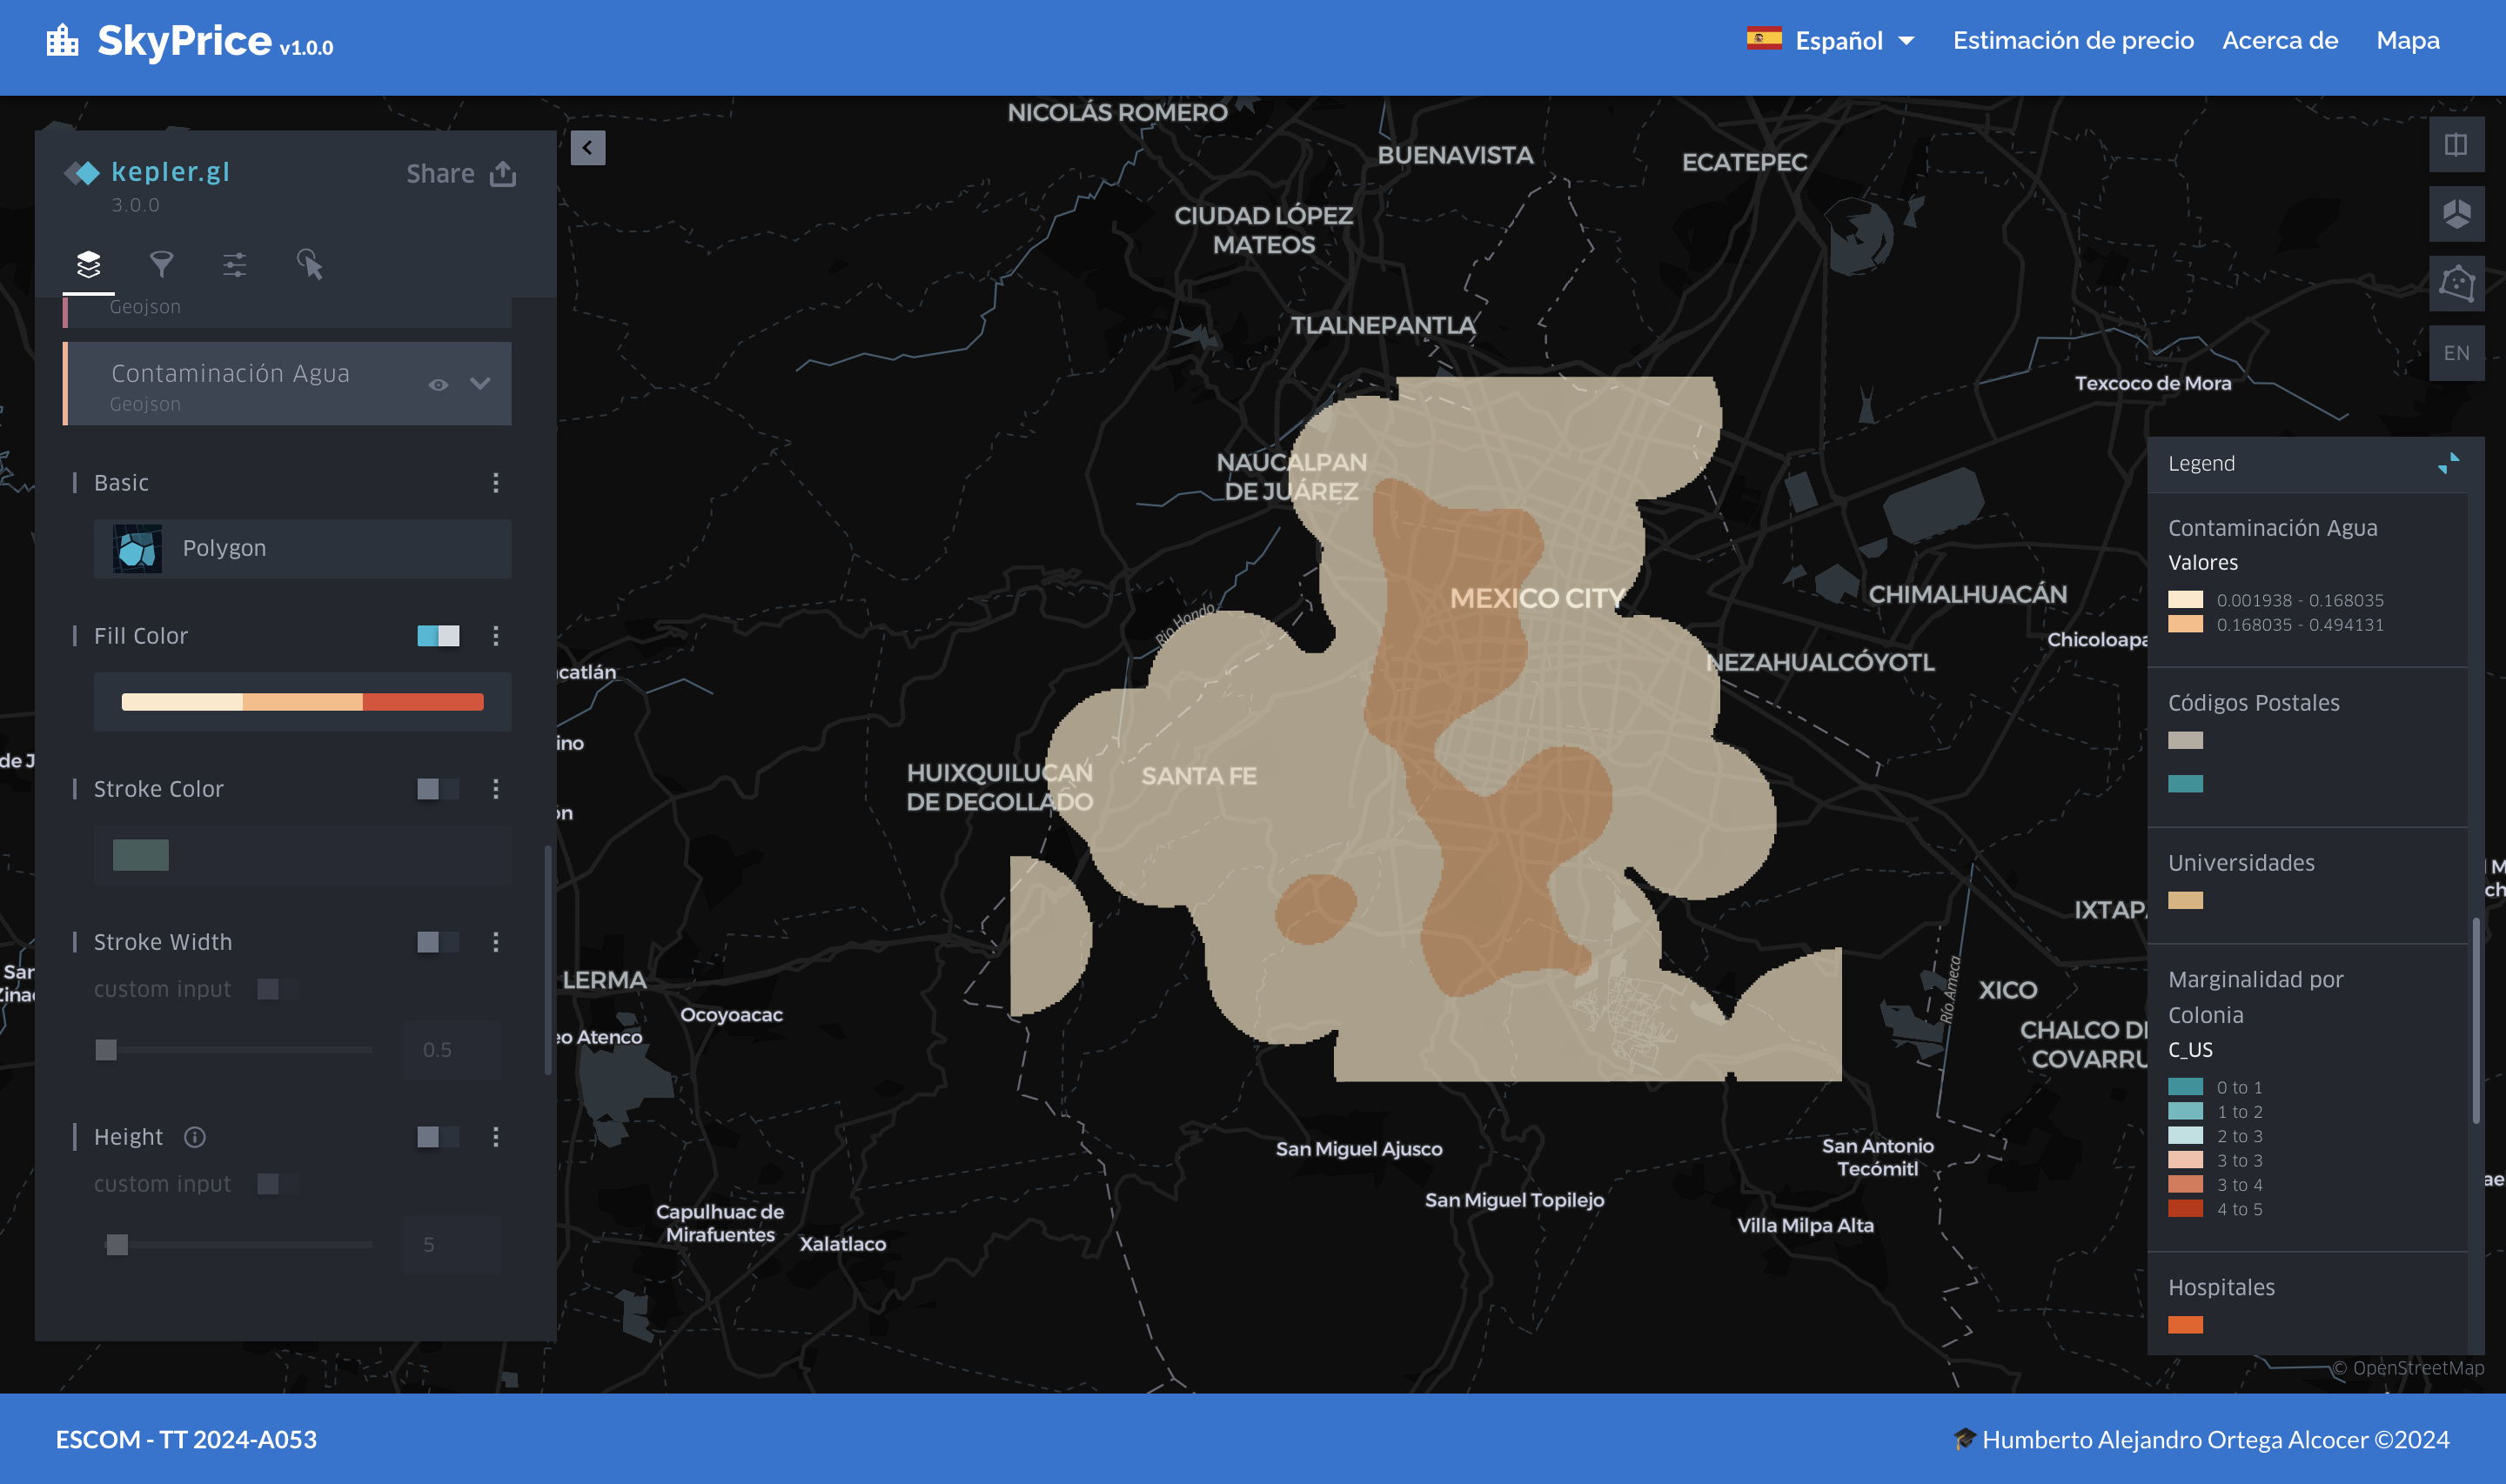
\includegraphics[width=0.8\textwidth]{imagenes/05-mapa-interactivo/contaminacion-agua.png}
    \caption{Contaminación del agua}
    \label{fig:contaminacion-agua}
\end{figure}

\subsection{Códigos postales}
Esta capa contiene los polígonos de los códigos postales de la Ciudad de México. En
la figura \ref{fig:codigos-postales} se muestra la capa de códigos postales.

\begin{figure}[H]
    \centering
    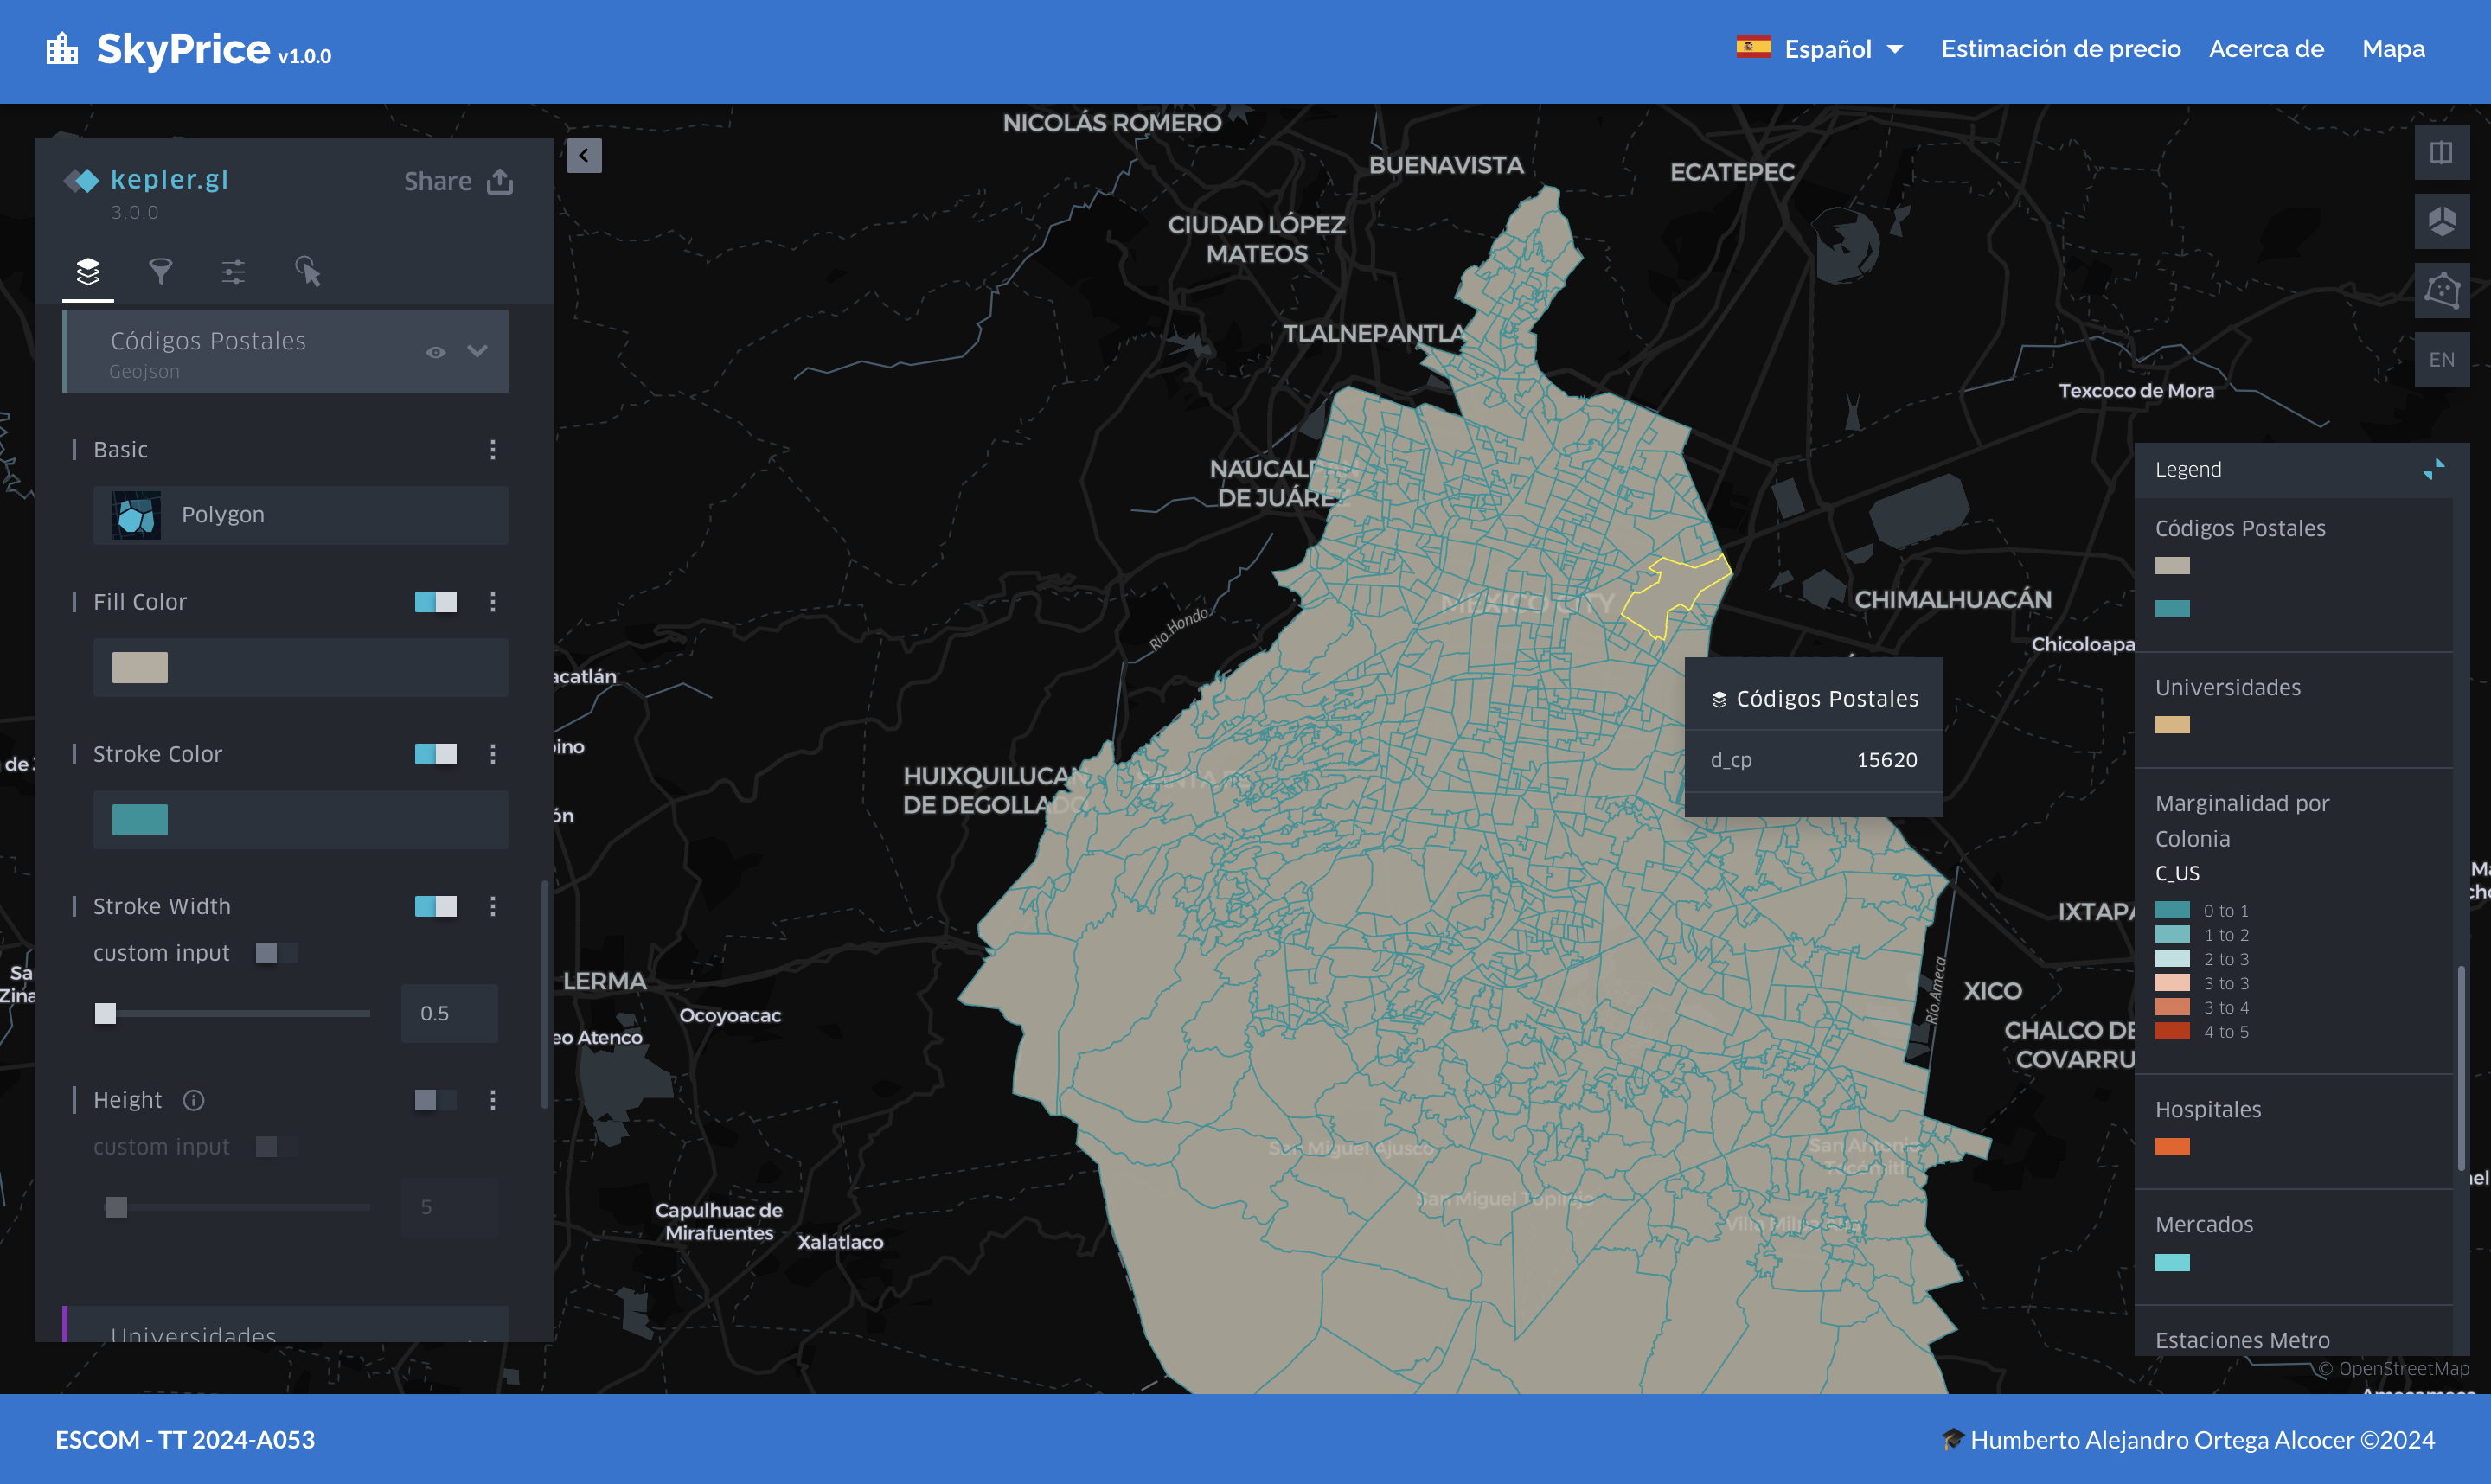
\includegraphics[width=0.8\textwidth]{imagenes/05-mapa-interactivo/codigos-postales.png}
    \caption{Códigos postales}
    \label{fig:codigos-postales}
\end{figure}

\subsection{Universidades}
Esta capa contiene la ubicación de universidades en la Ciudad de México. En la
figura \ref{fig:universidades} se muestra la capa de universidades.

\begin{figure}[H]
    \centering
    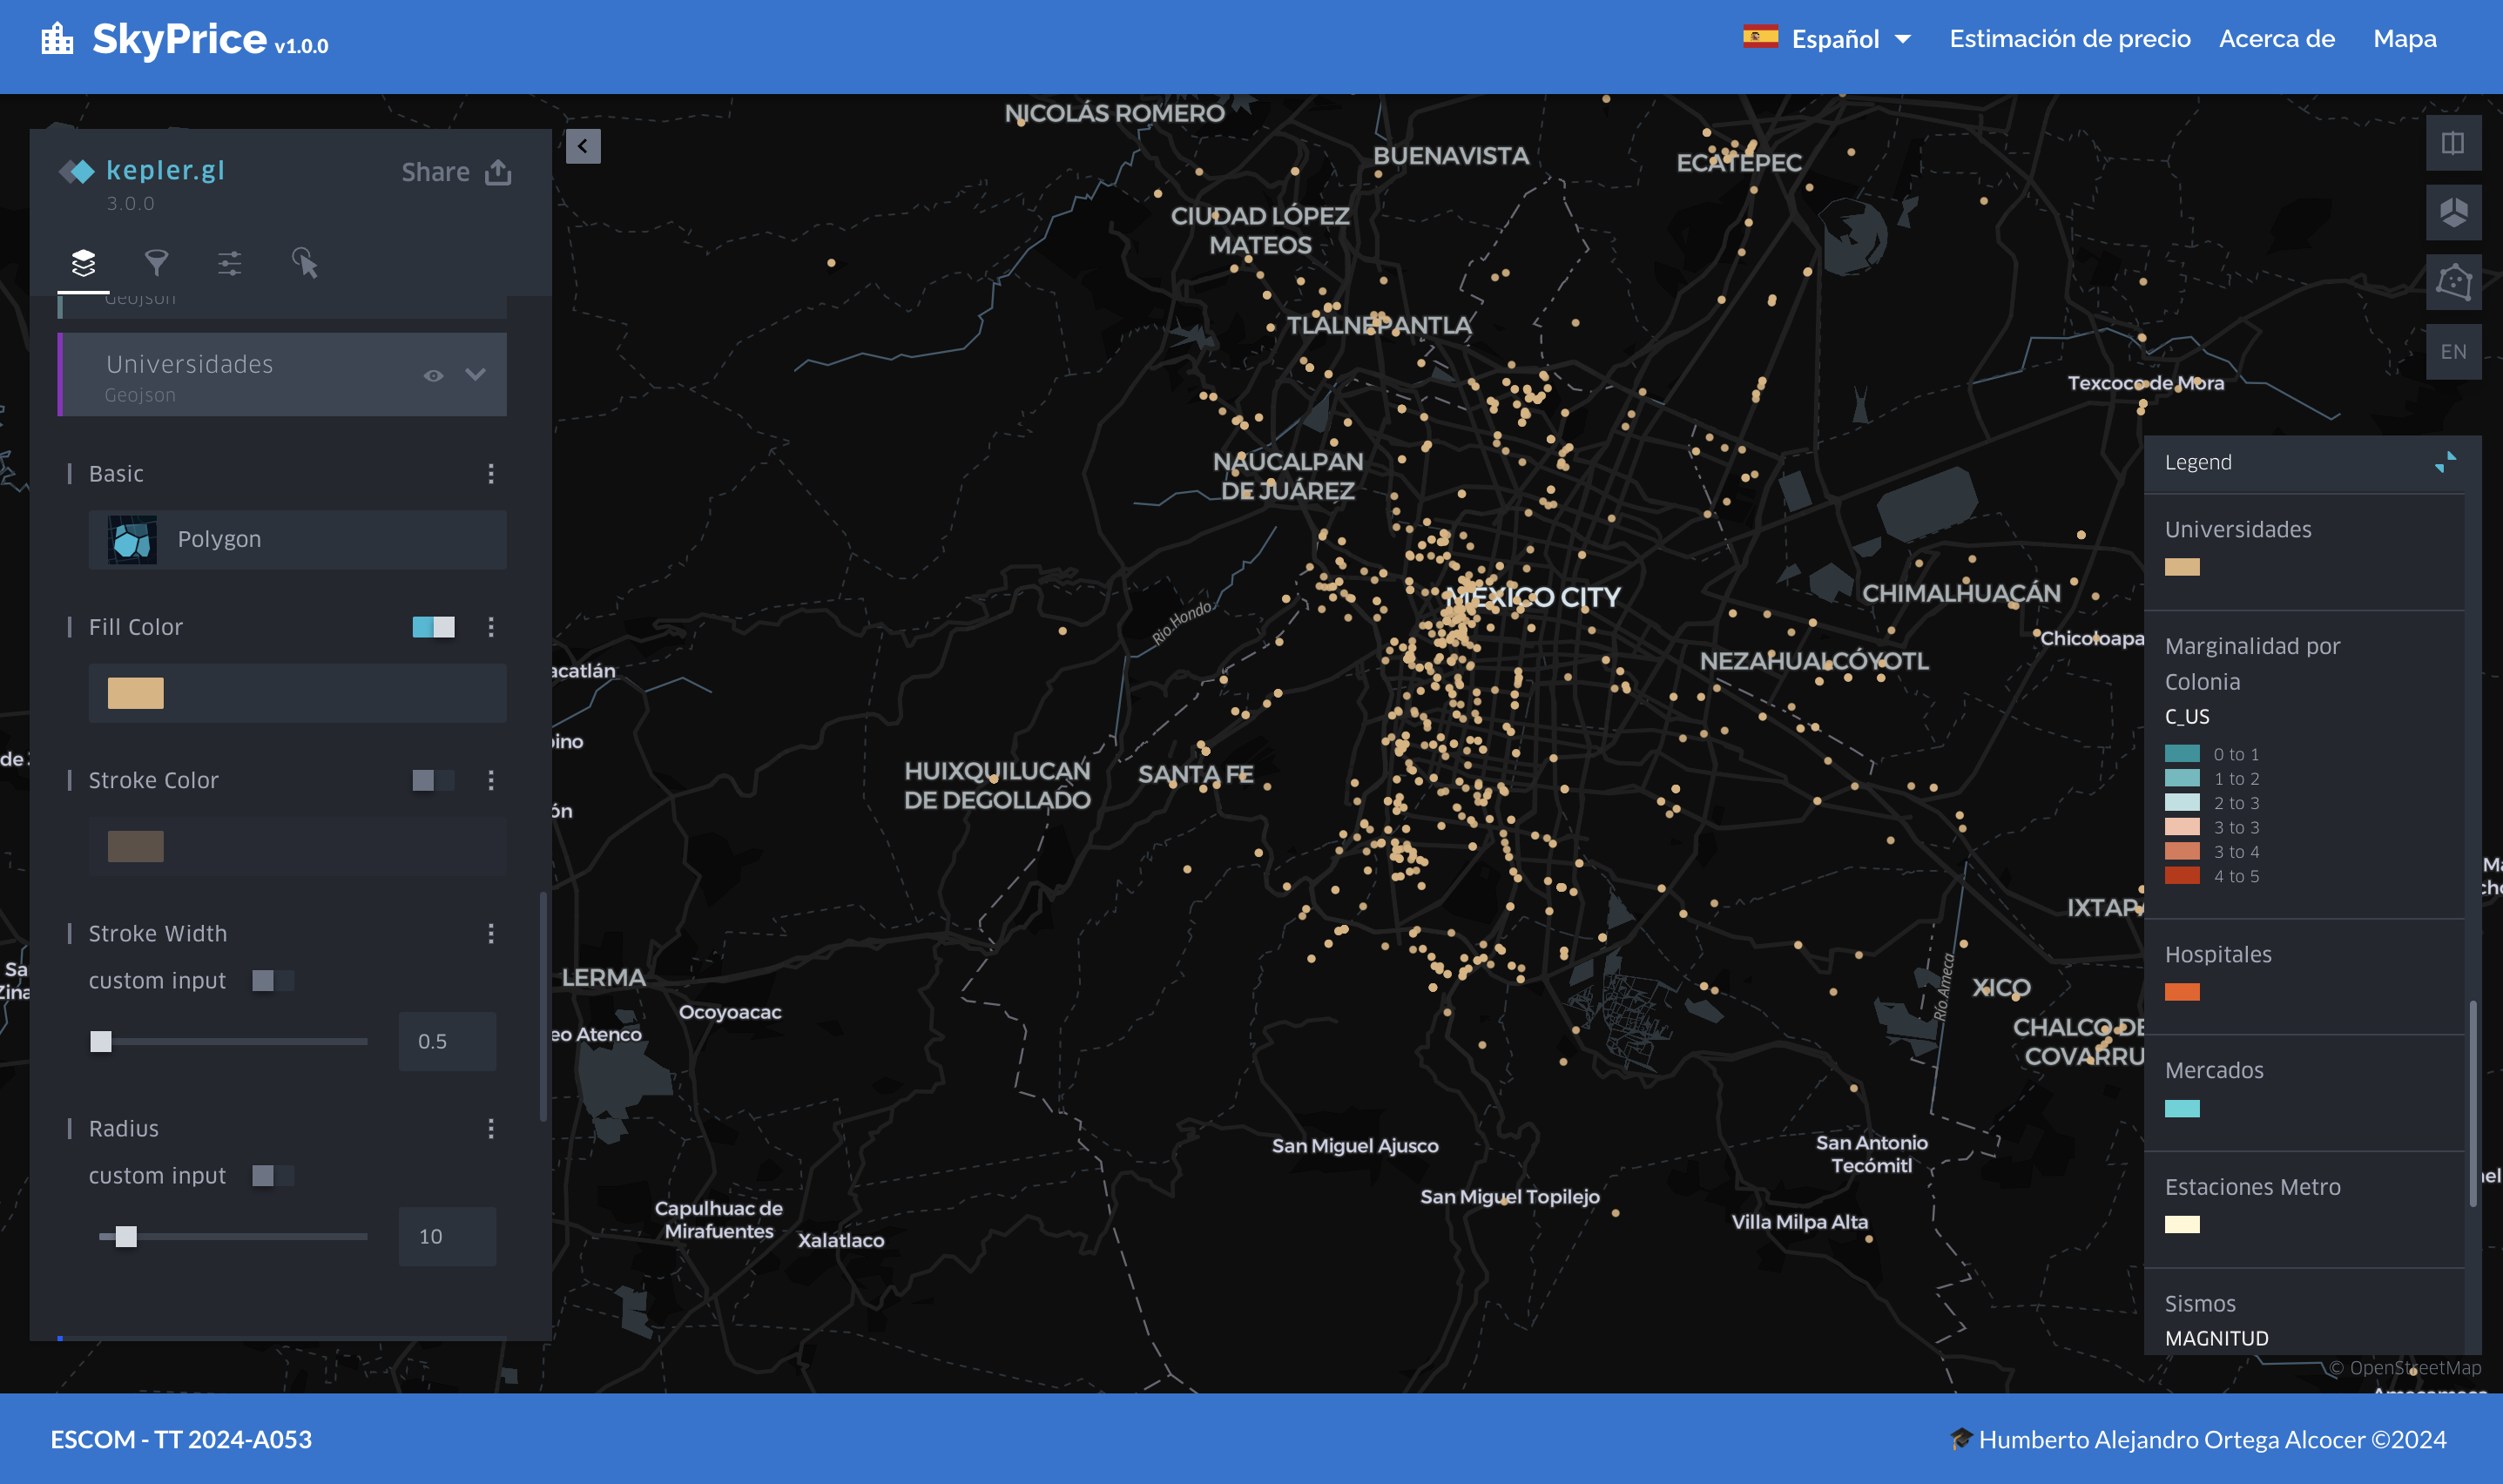
\includegraphics[width=0.8\textwidth]{imagenes/05-mapa-interactivo/universidades.png}
    \caption{Universidades}
    \label{fig:universidades}
\end{figure}

\subsection{Marginalidad}
Esta capa contiene los polígonos con los niveles de marginalidad en la Ciudad de
México. En la figura \ref{fig:marginalidad} se muestra la capa de marginalidad.

\begin{figure}[H]
    \centering
    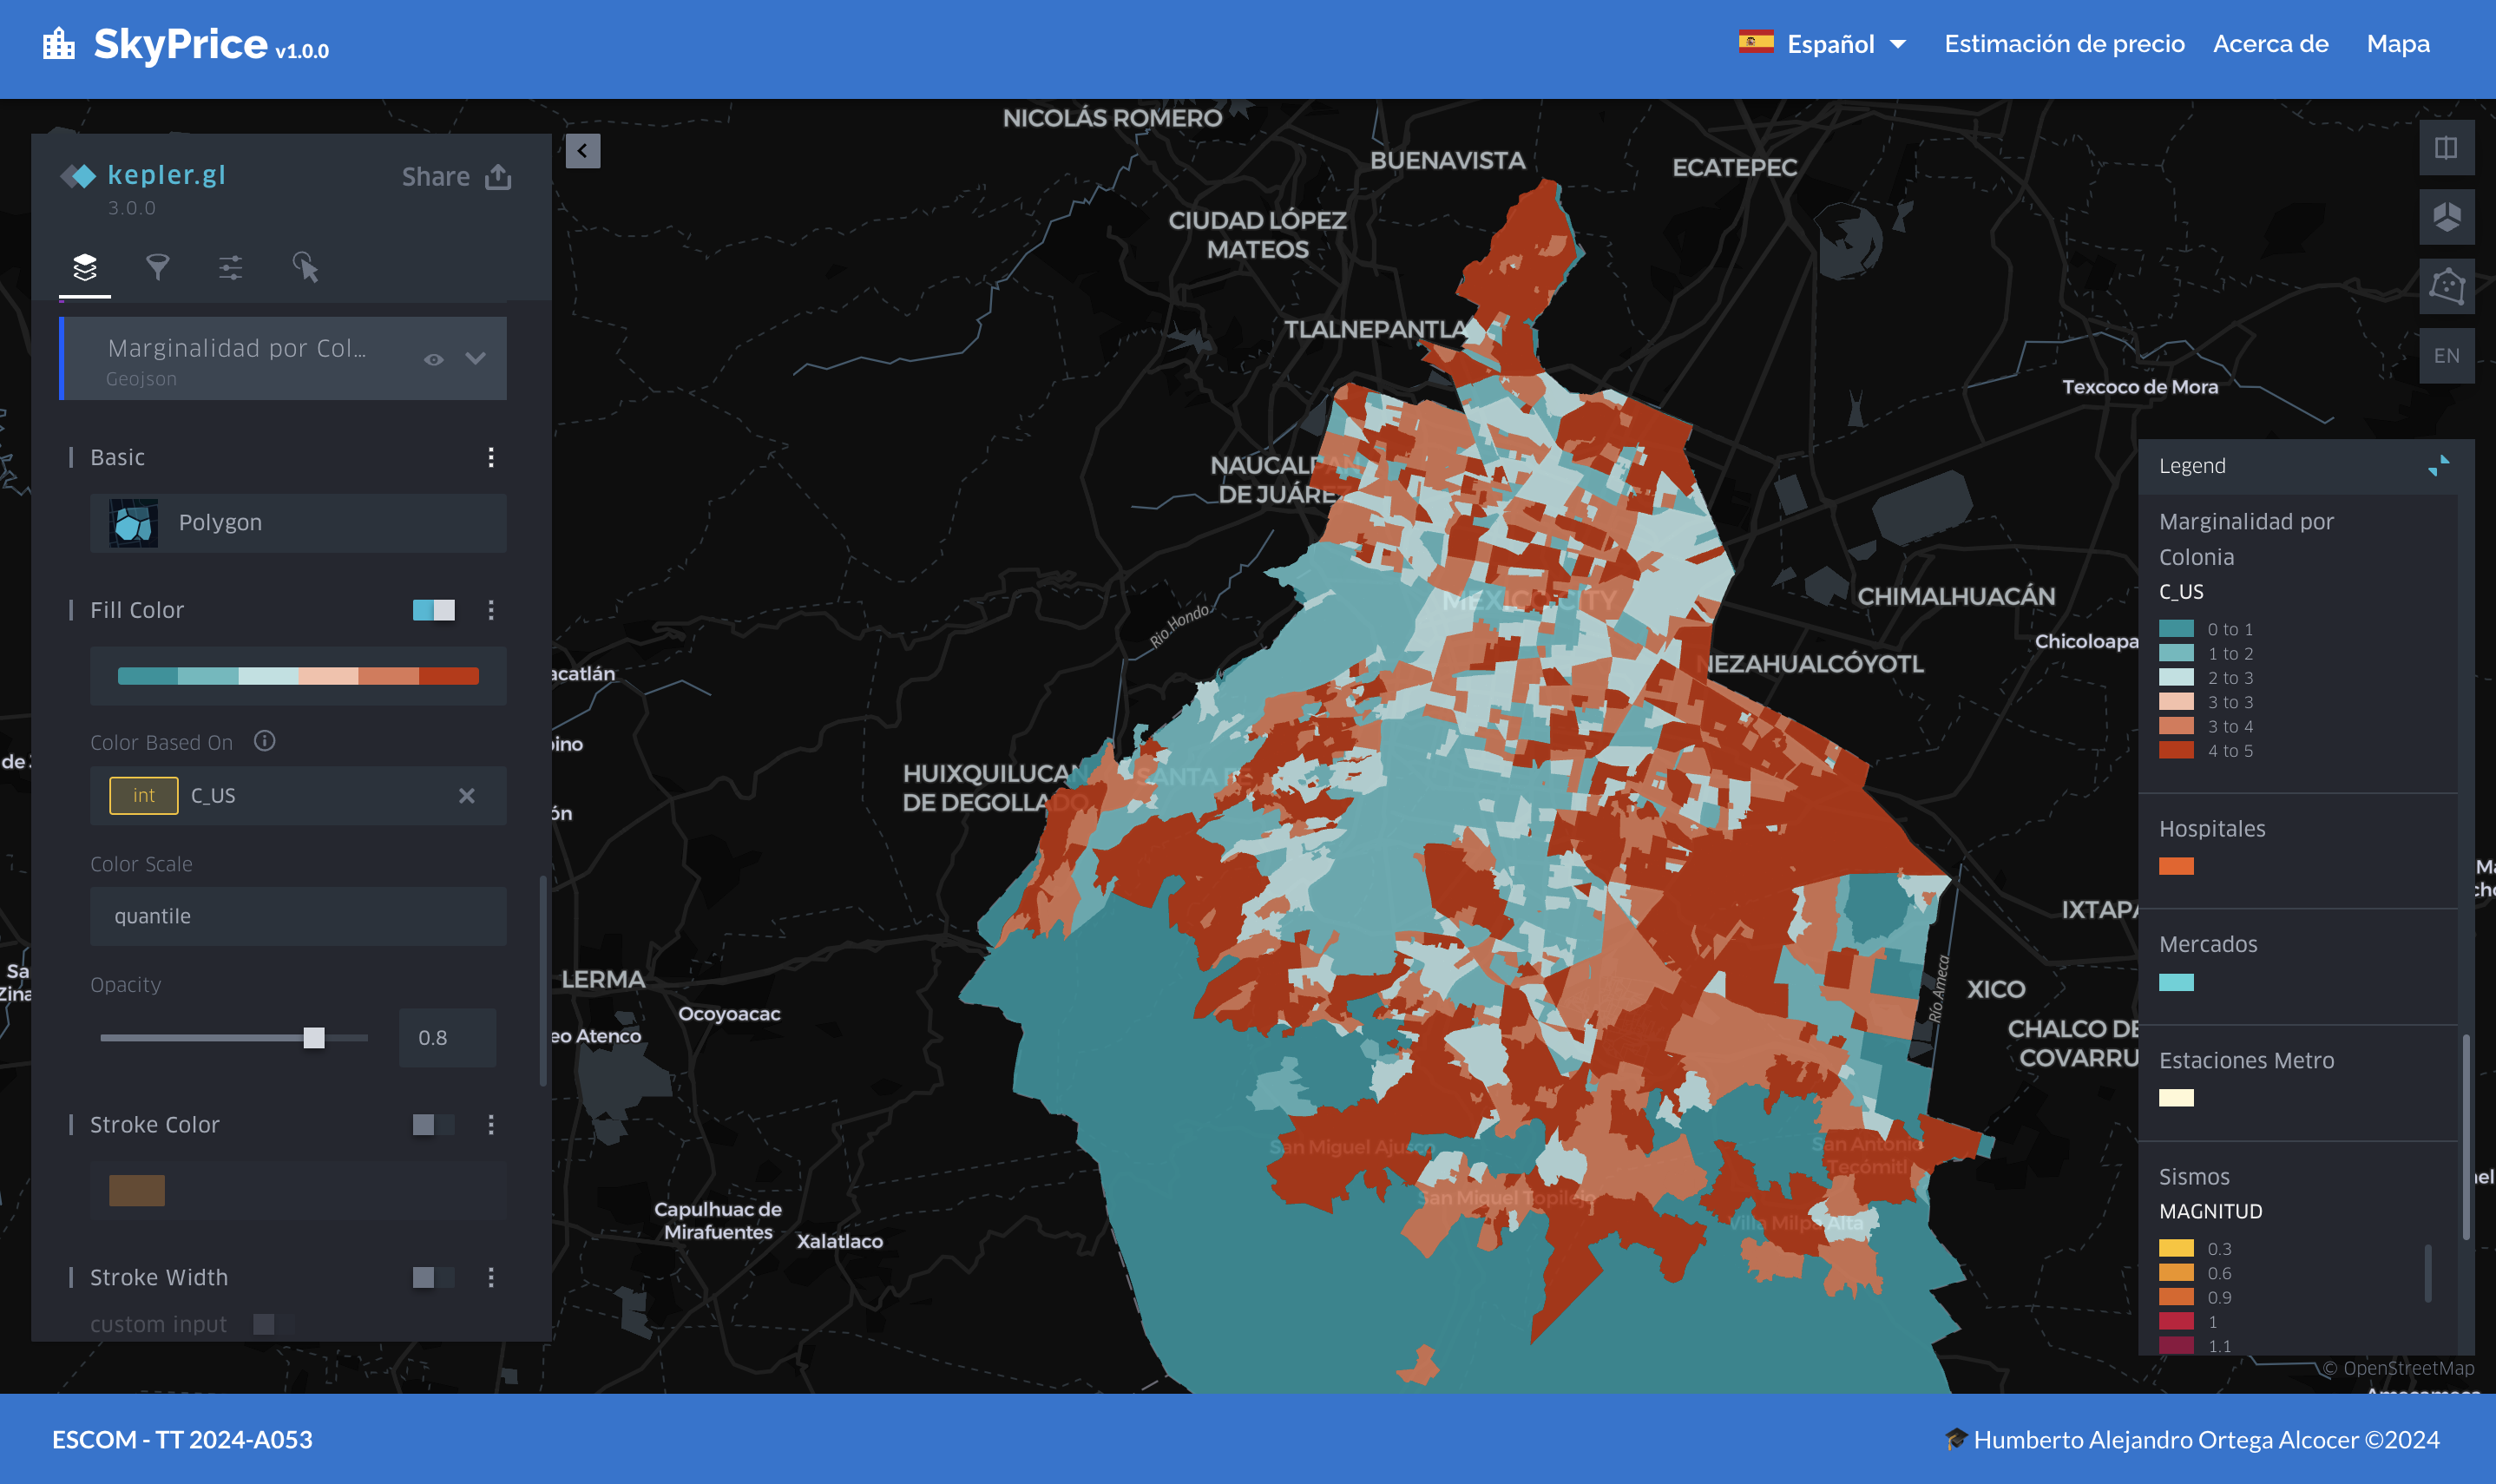
\includegraphics[width=0.8\textwidth]{imagenes/05-mapa-interactivo/marginalidad.png}
    \caption{Marginalidad}
    \label{fig:marginalidad}
\end{figure}

\subsection{Hospitales}
Esta capa contiene la ubicación de hospitales en la Ciudad de México. En la figura
\ref{fig:hospitales} se muestra la capa de hospitales.

\begin{figure}[H]
    \centering
    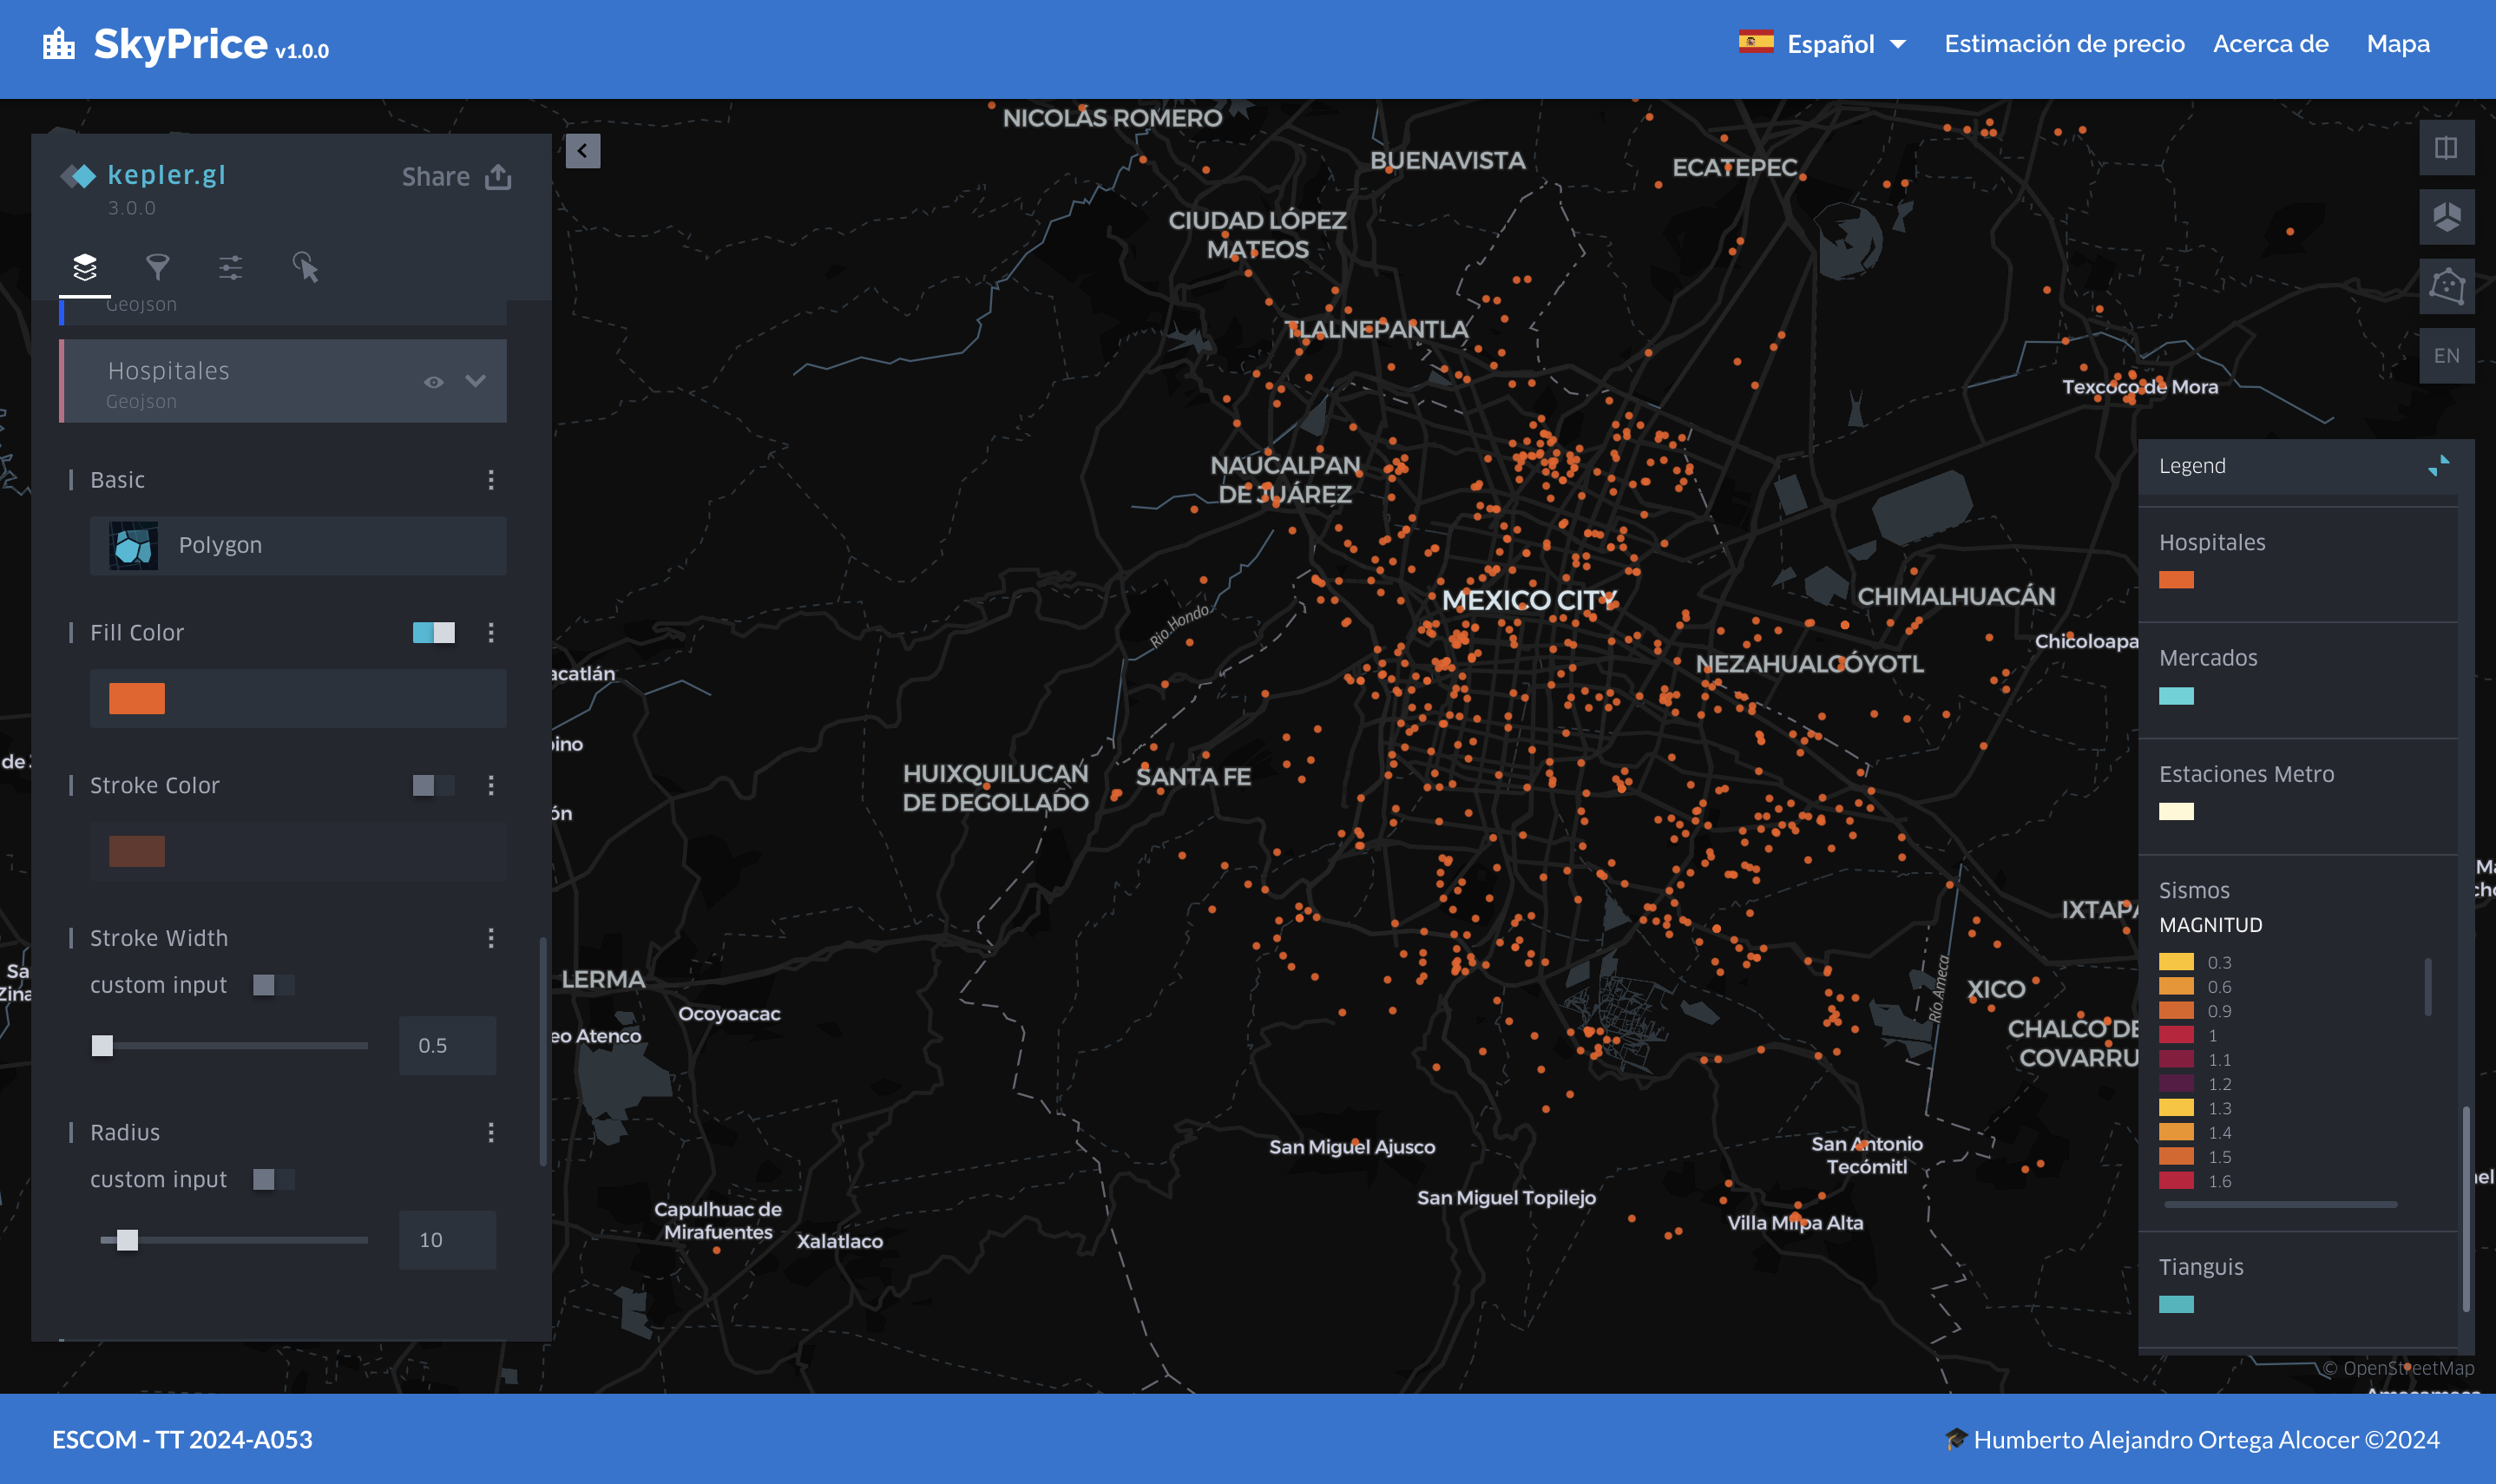
\includegraphics[width=0.8\textwidth]{imagenes/05-mapa-interactivo/hospitales.png}
    \caption{Hospitales}
    \label{fig:hospitales}
\end{figure}

\subsection{Mercados}
Esta capa contiene la ubicación de mercados en la Ciudad de México. En la figura
\ref{fig:mercados} se muestra la capa de mercados.

\begin{figure}[H]
    \centering
    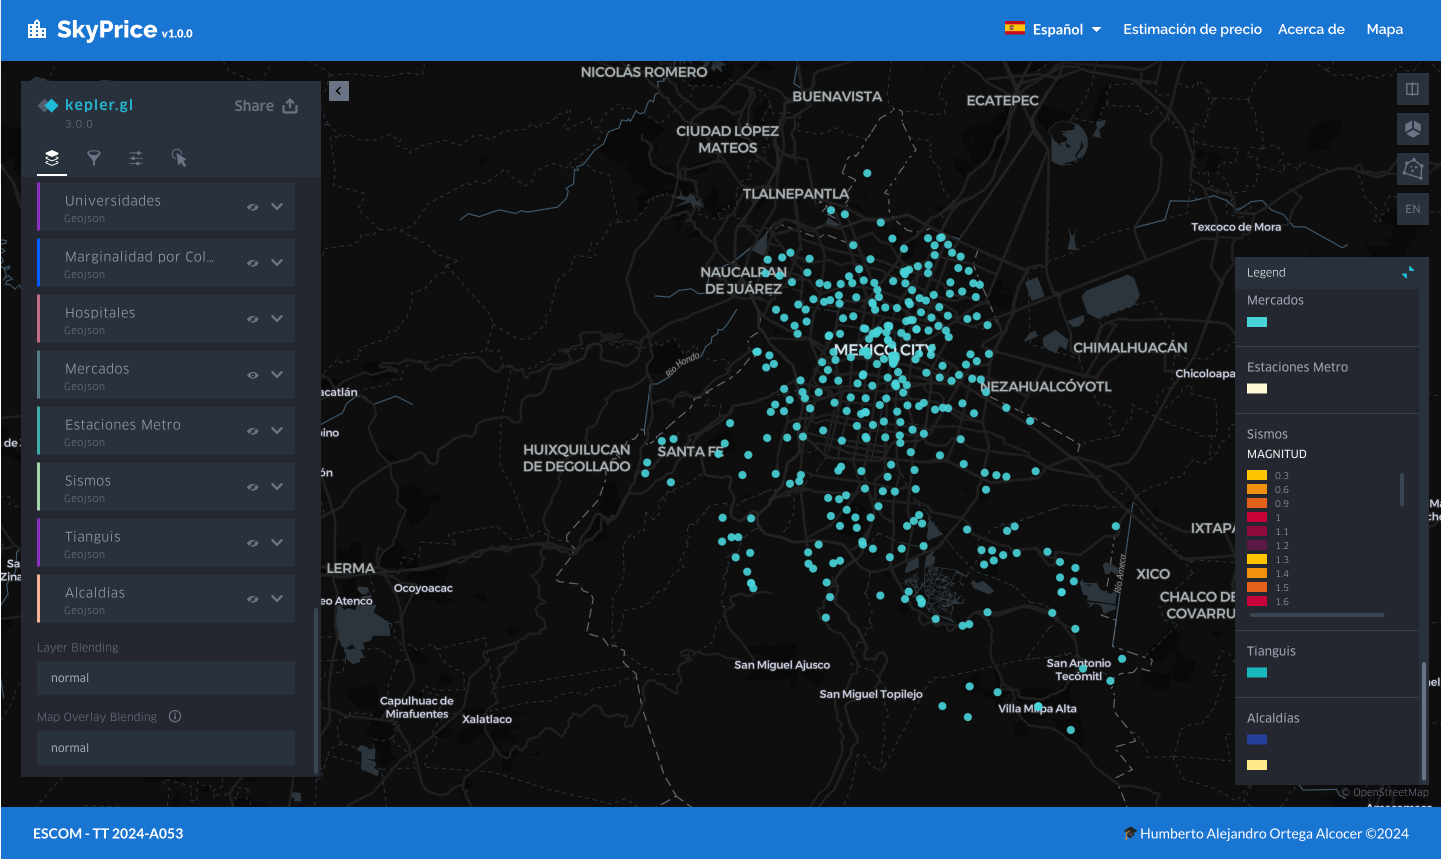
\includegraphics[width=0.8\textwidth]{imagenes/05-mapa-interactivo/mercados.png}
    \caption{Mercados}
    \label{fig:mercados}
\end{figure}

\subsection{Metro}
Esta capa contiene la ubicación de las estaciones del metro en la Ciudad de México.
En la figura \ref{fig:metro} se muestra la capa de metro.

\begin{figure}[H]
    \centering
    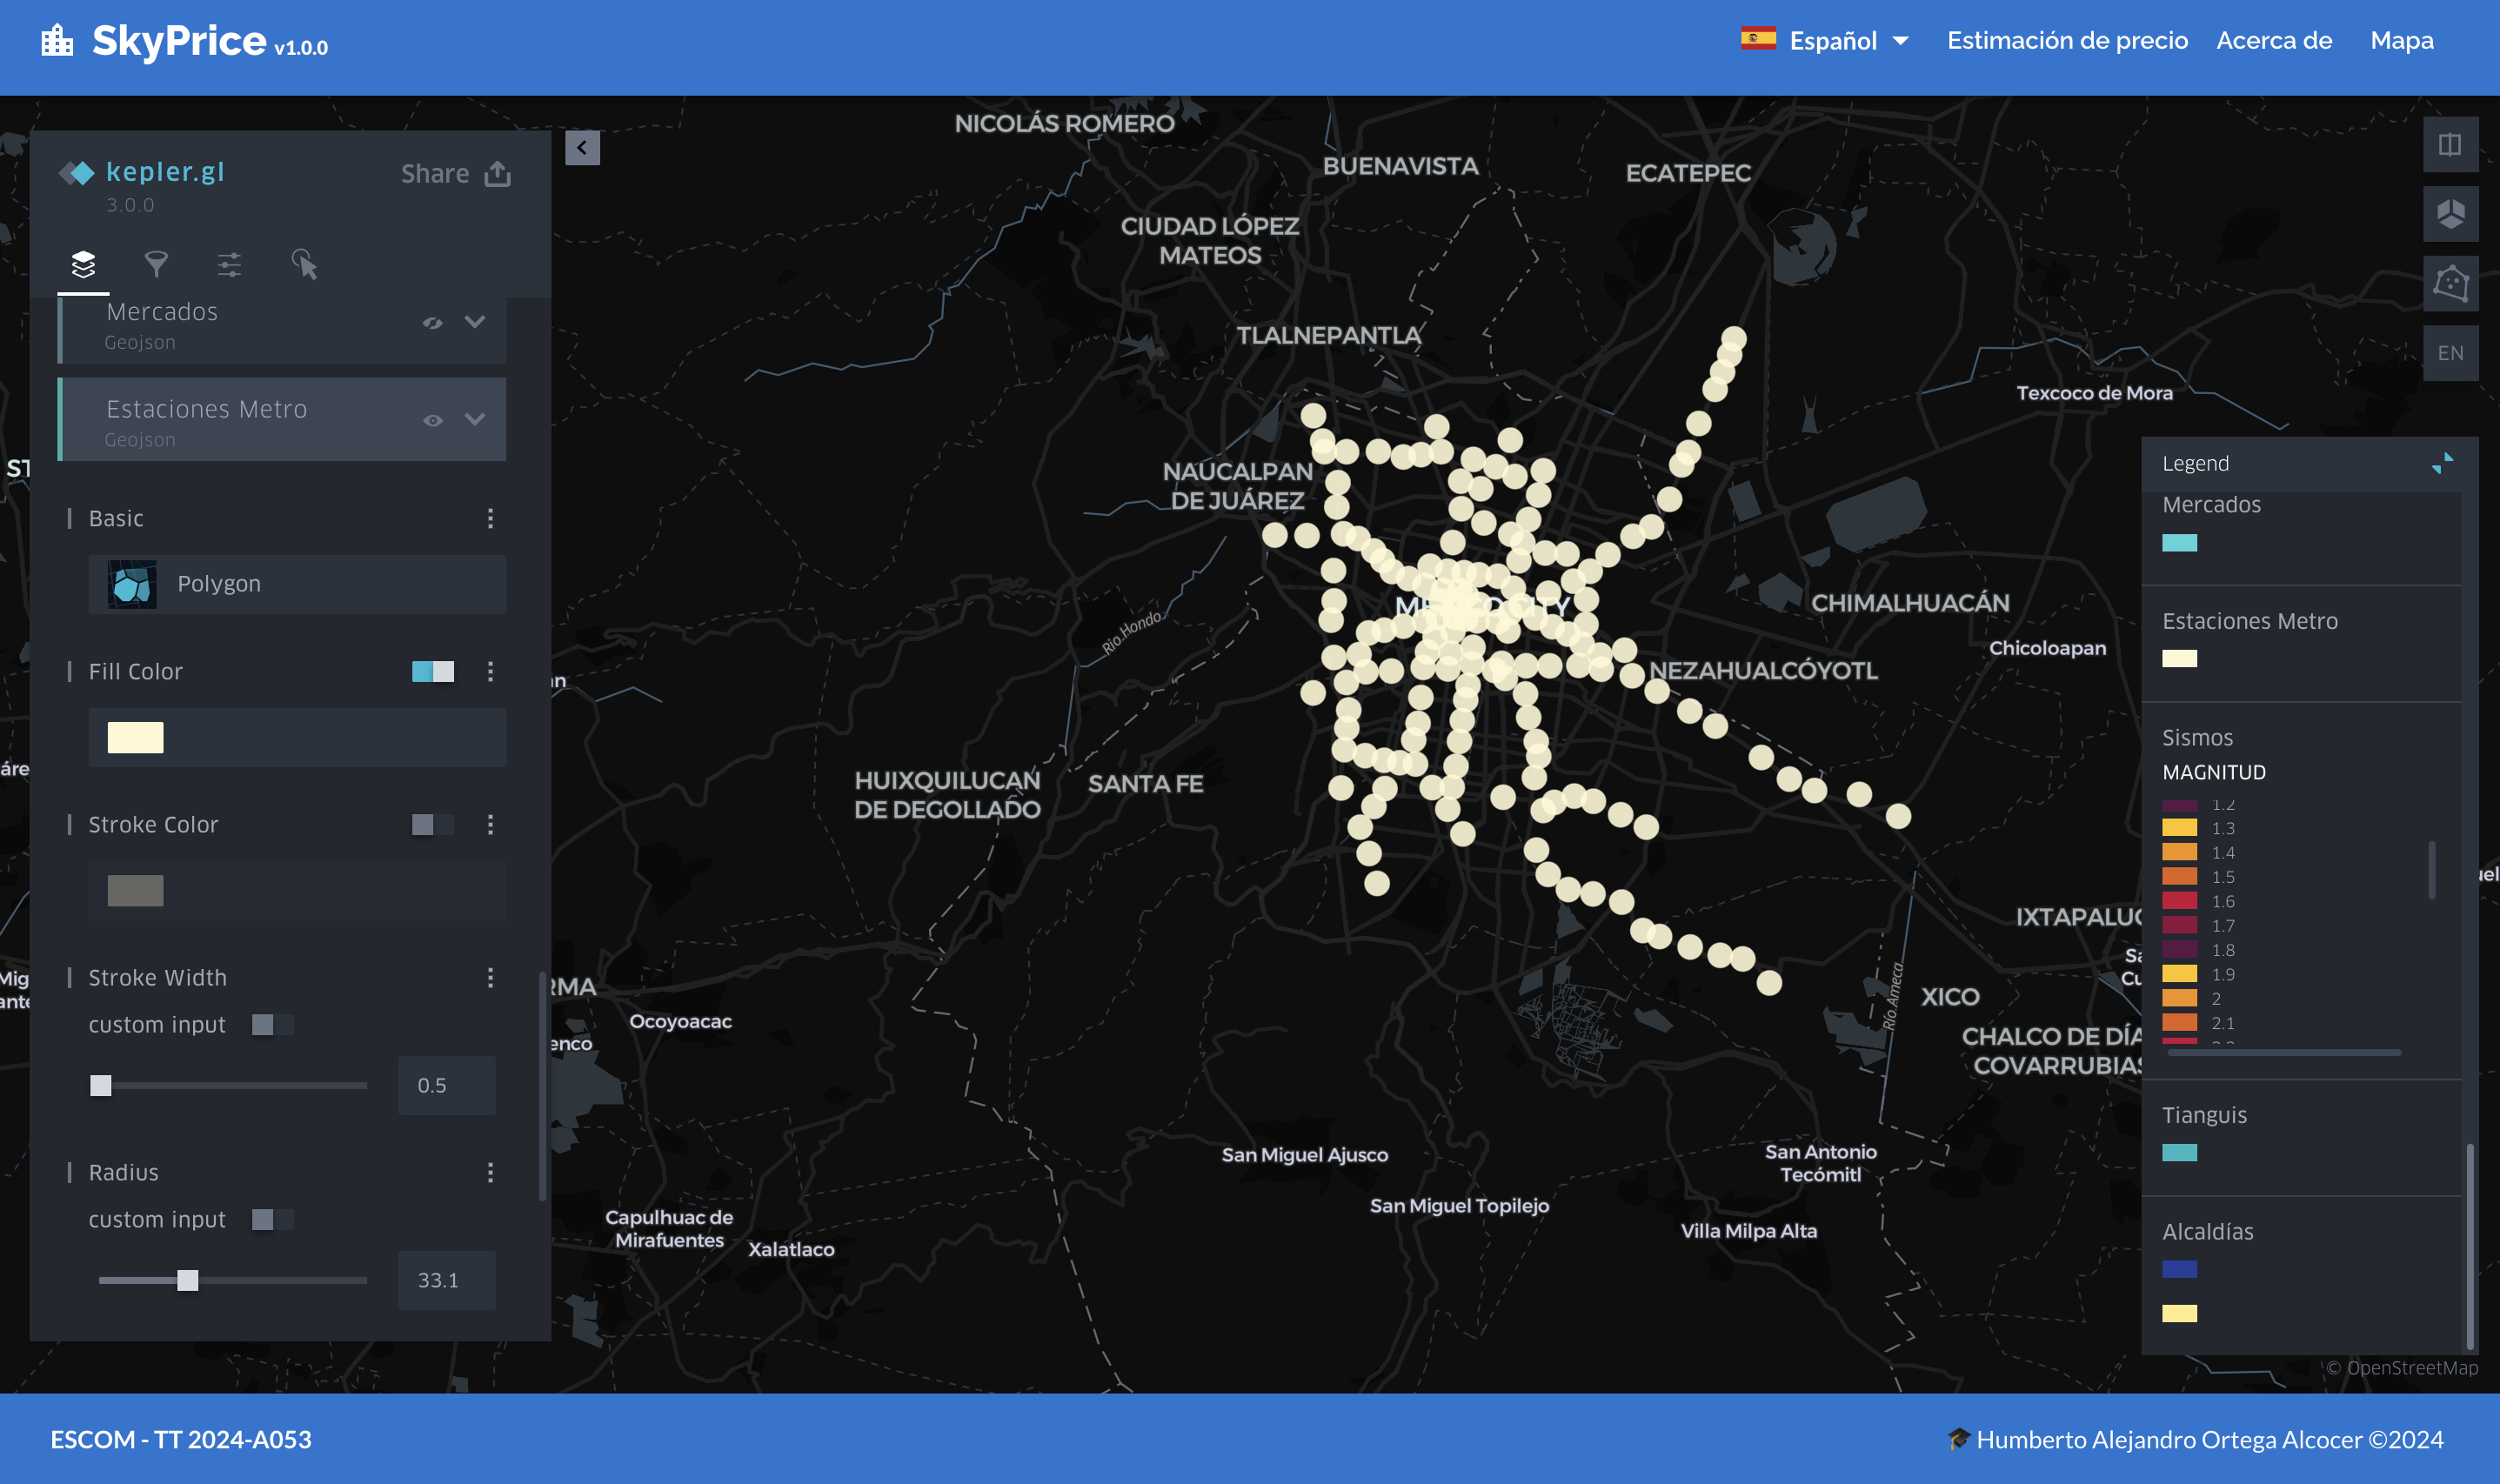
\includegraphics[width=0.8\textwidth]{imagenes/05-mapa-interactivo/metro.png}
    \caption{Metro}
    \label{fig:metro}
\end{figure}

\subsection{Sismos}
Esta capa contiene la ubicación de los sismos en la Ciudad de México. En la figura
\ref{fig:sismos} se muestra la capa de sismos.

\begin{figure}[H]
    \centering
    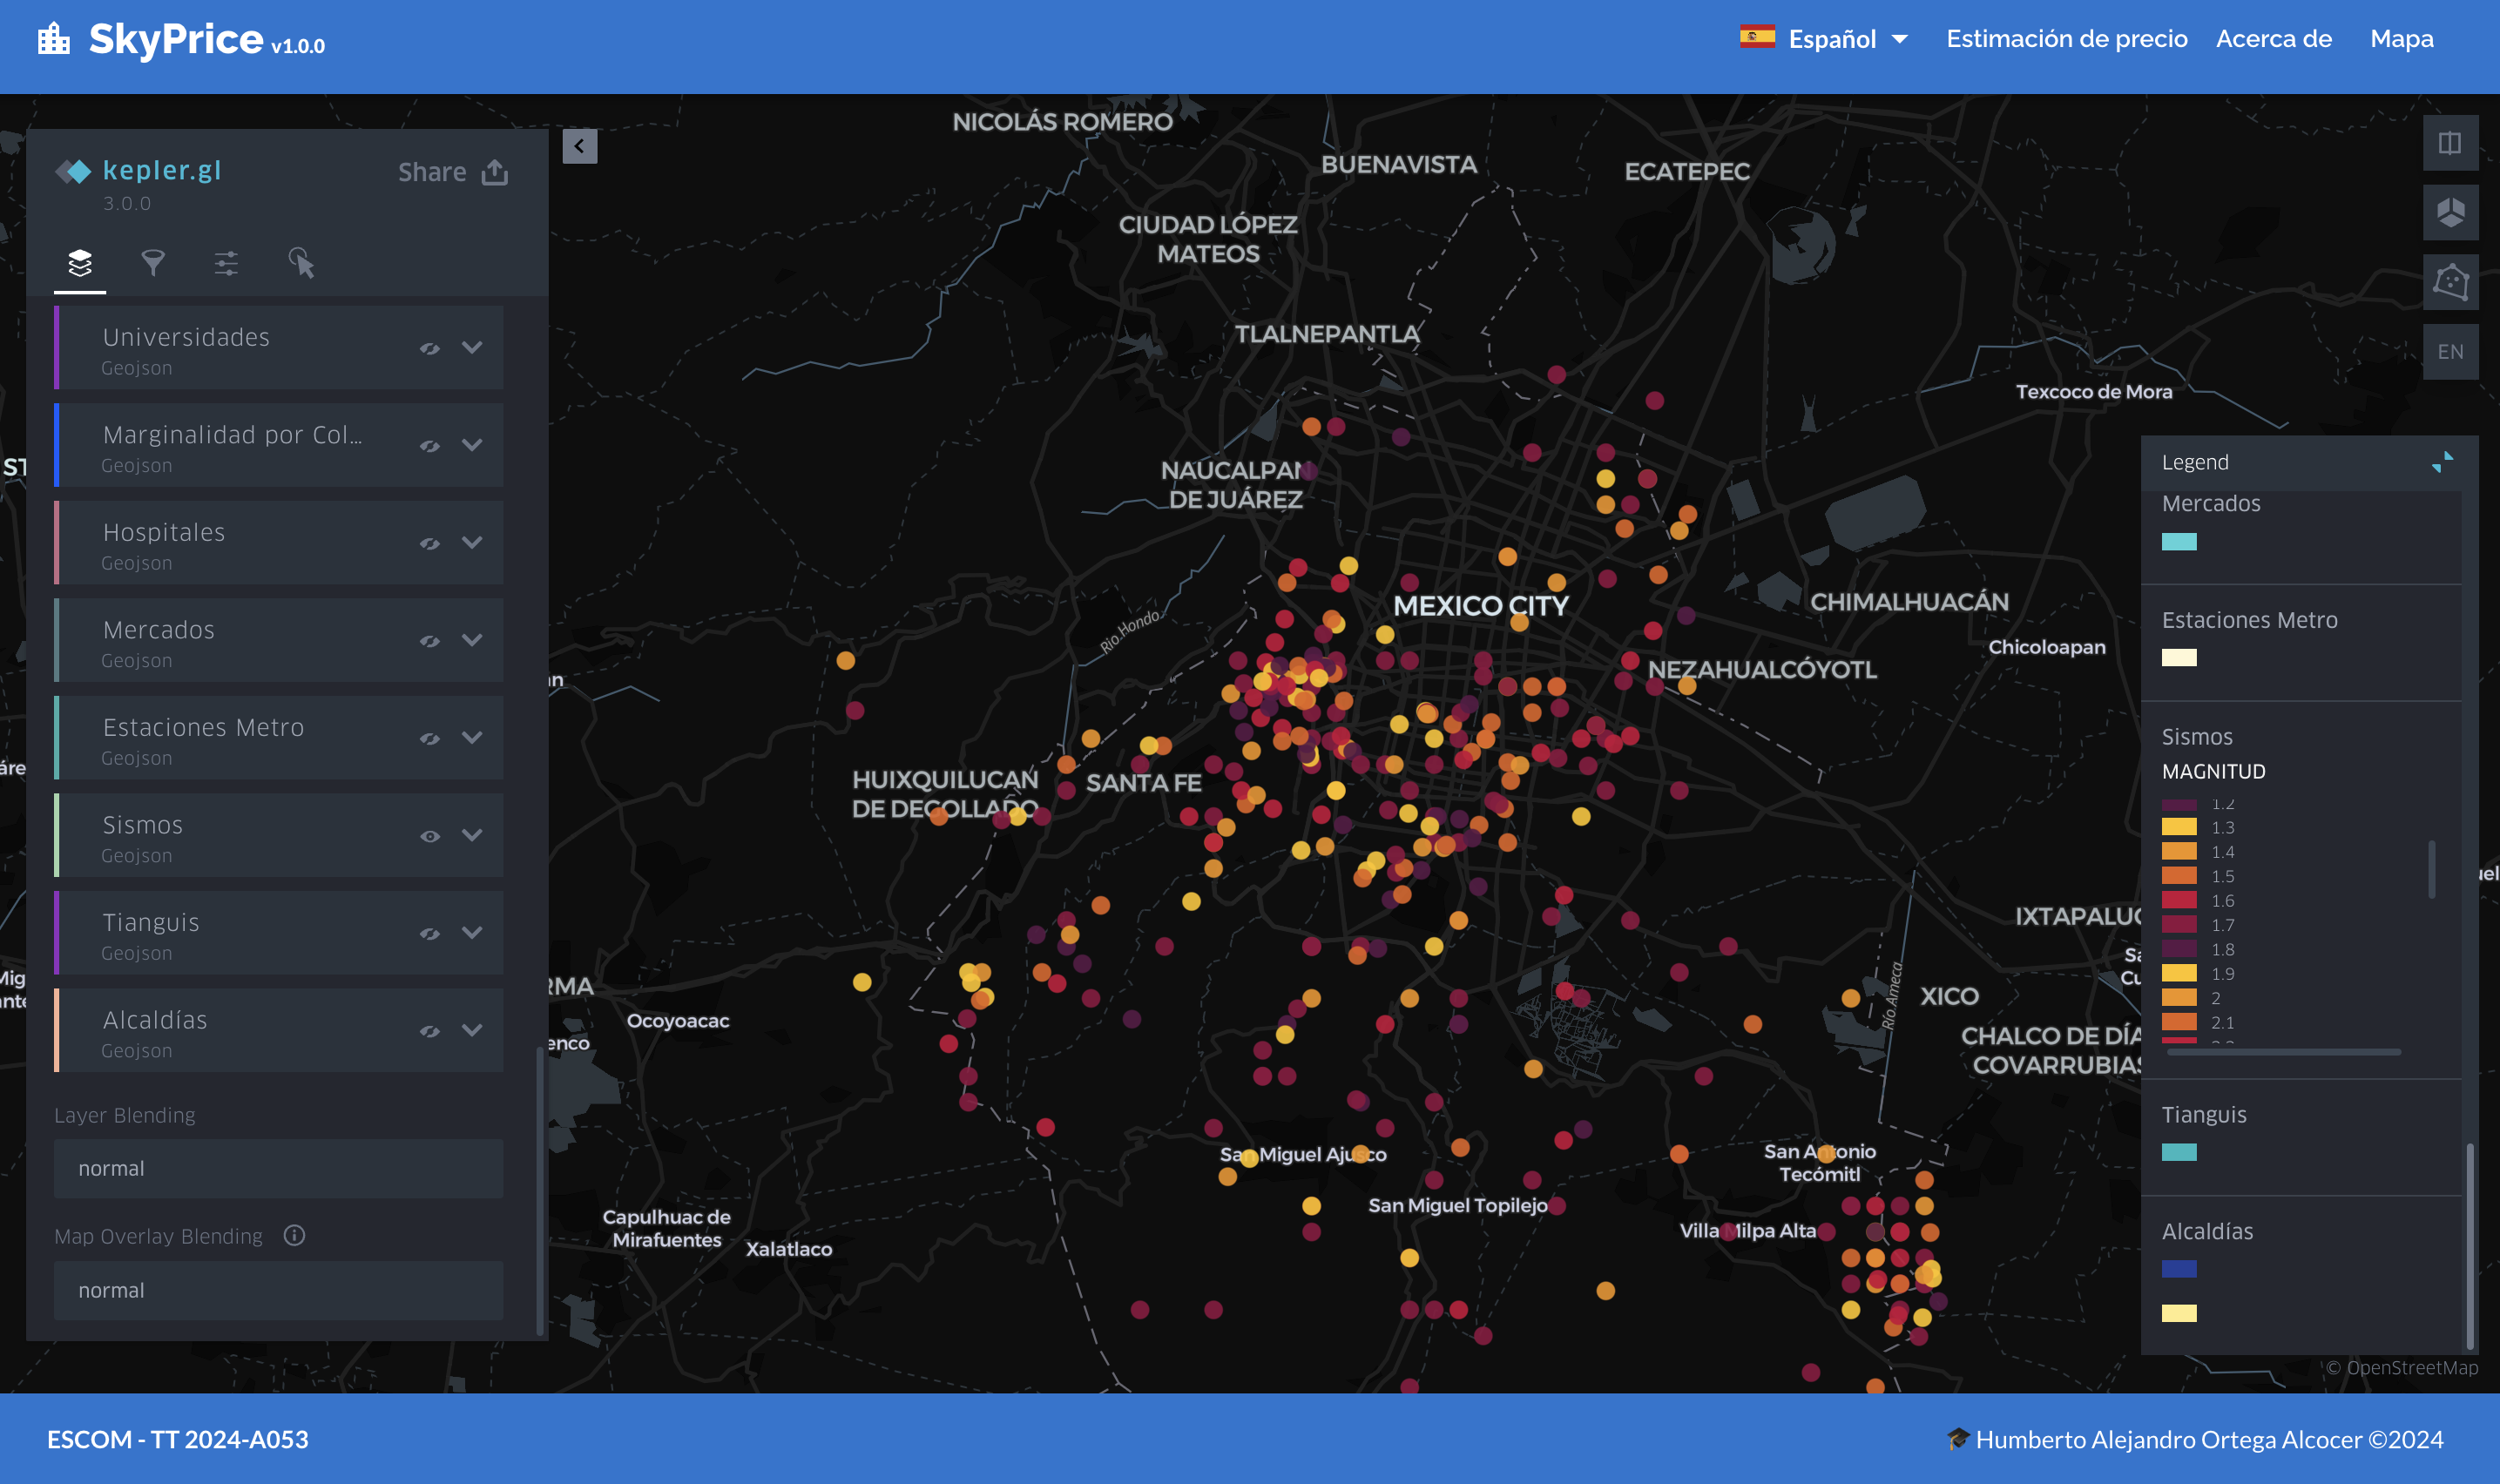
\includegraphics[width=0.8\textwidth]{imagenes/05-mapa-interactivo/sismos.png}
    \caption{Sismos}
    \label{fig:sismos}
\end{figure}

\subsection{Tianguis}
Esta capa contiene la ubicación de tianguis en la Ciudad de México. En la figura
\ref{fig:tianguis} se muestra la capa de tianguis.

\begin{figure}[H]
    \centering
    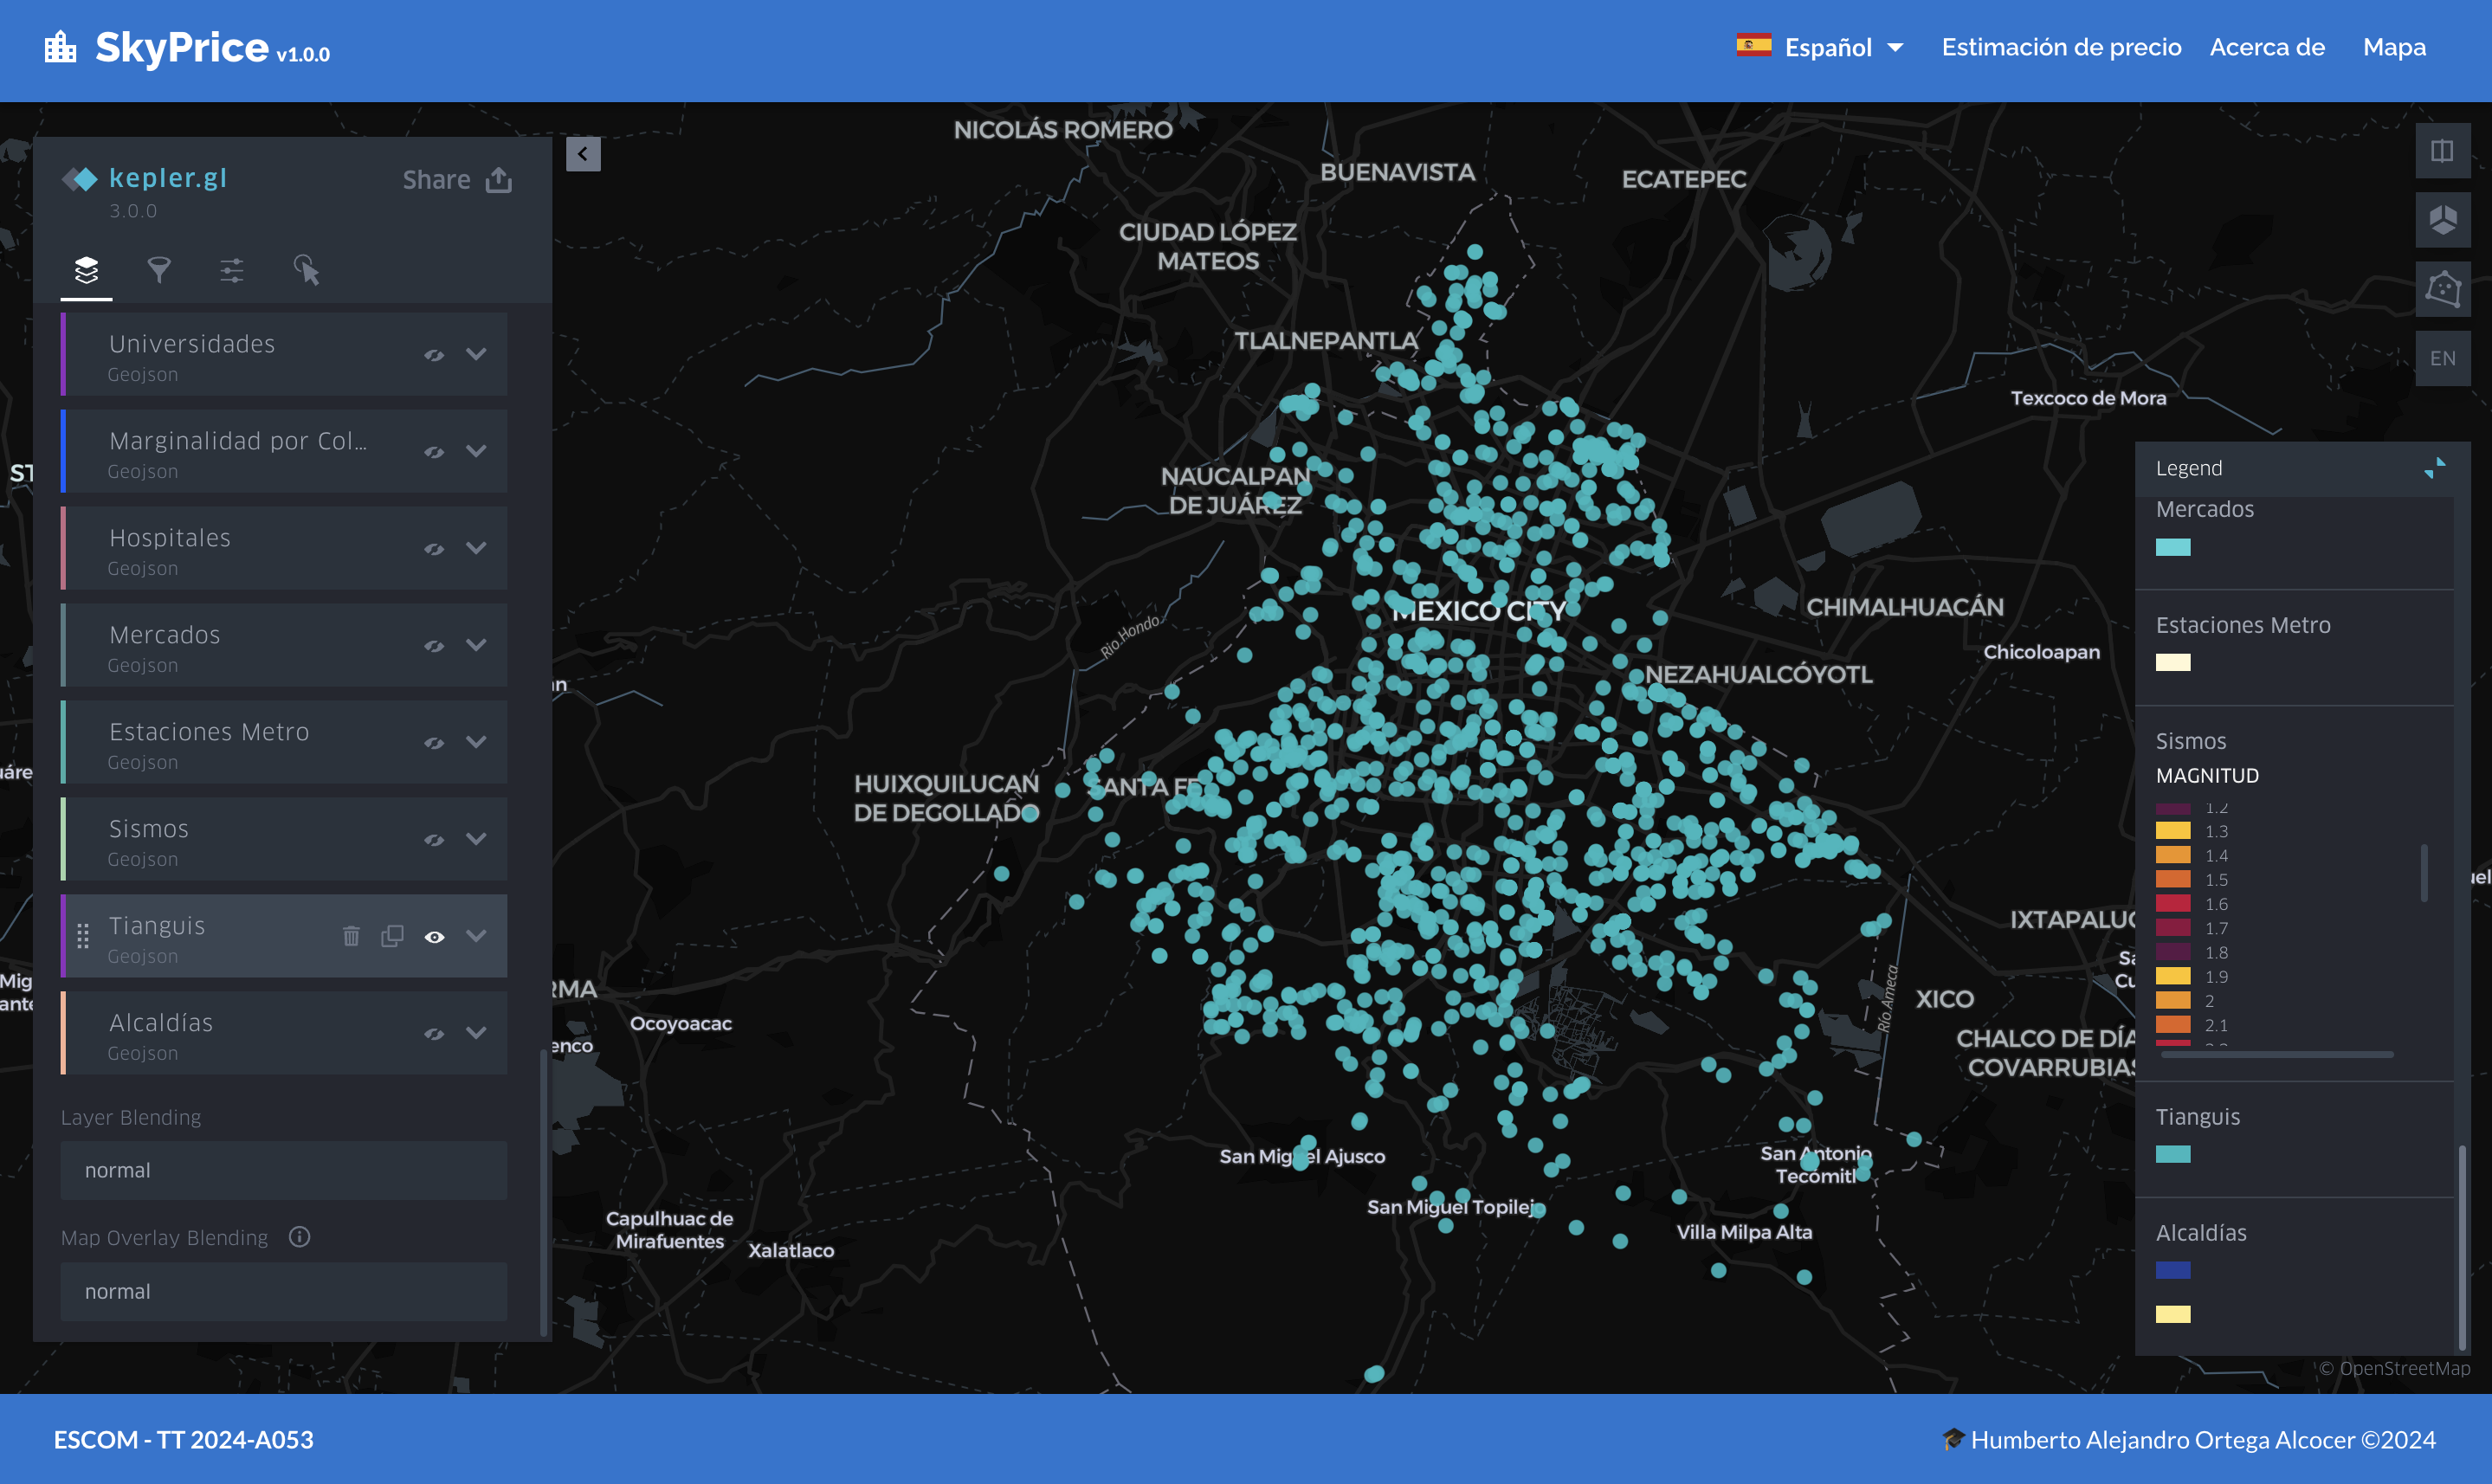
\includegraphics[width=0.8\textwidth]{imagenes/05-mapa-interactivo/tianguis.png}
    \caption{Tianguis}
    \label{fig:tianguis}
\end{figure}

\subsection{Alcaldías}
Esta capa contiene los polígonos de las alcaldías de la Ciudad de México. En la figura
\ref{fig:alcaldias} se muestra la capa de alcaldías.

\begin{figure}[H]
    \centering
    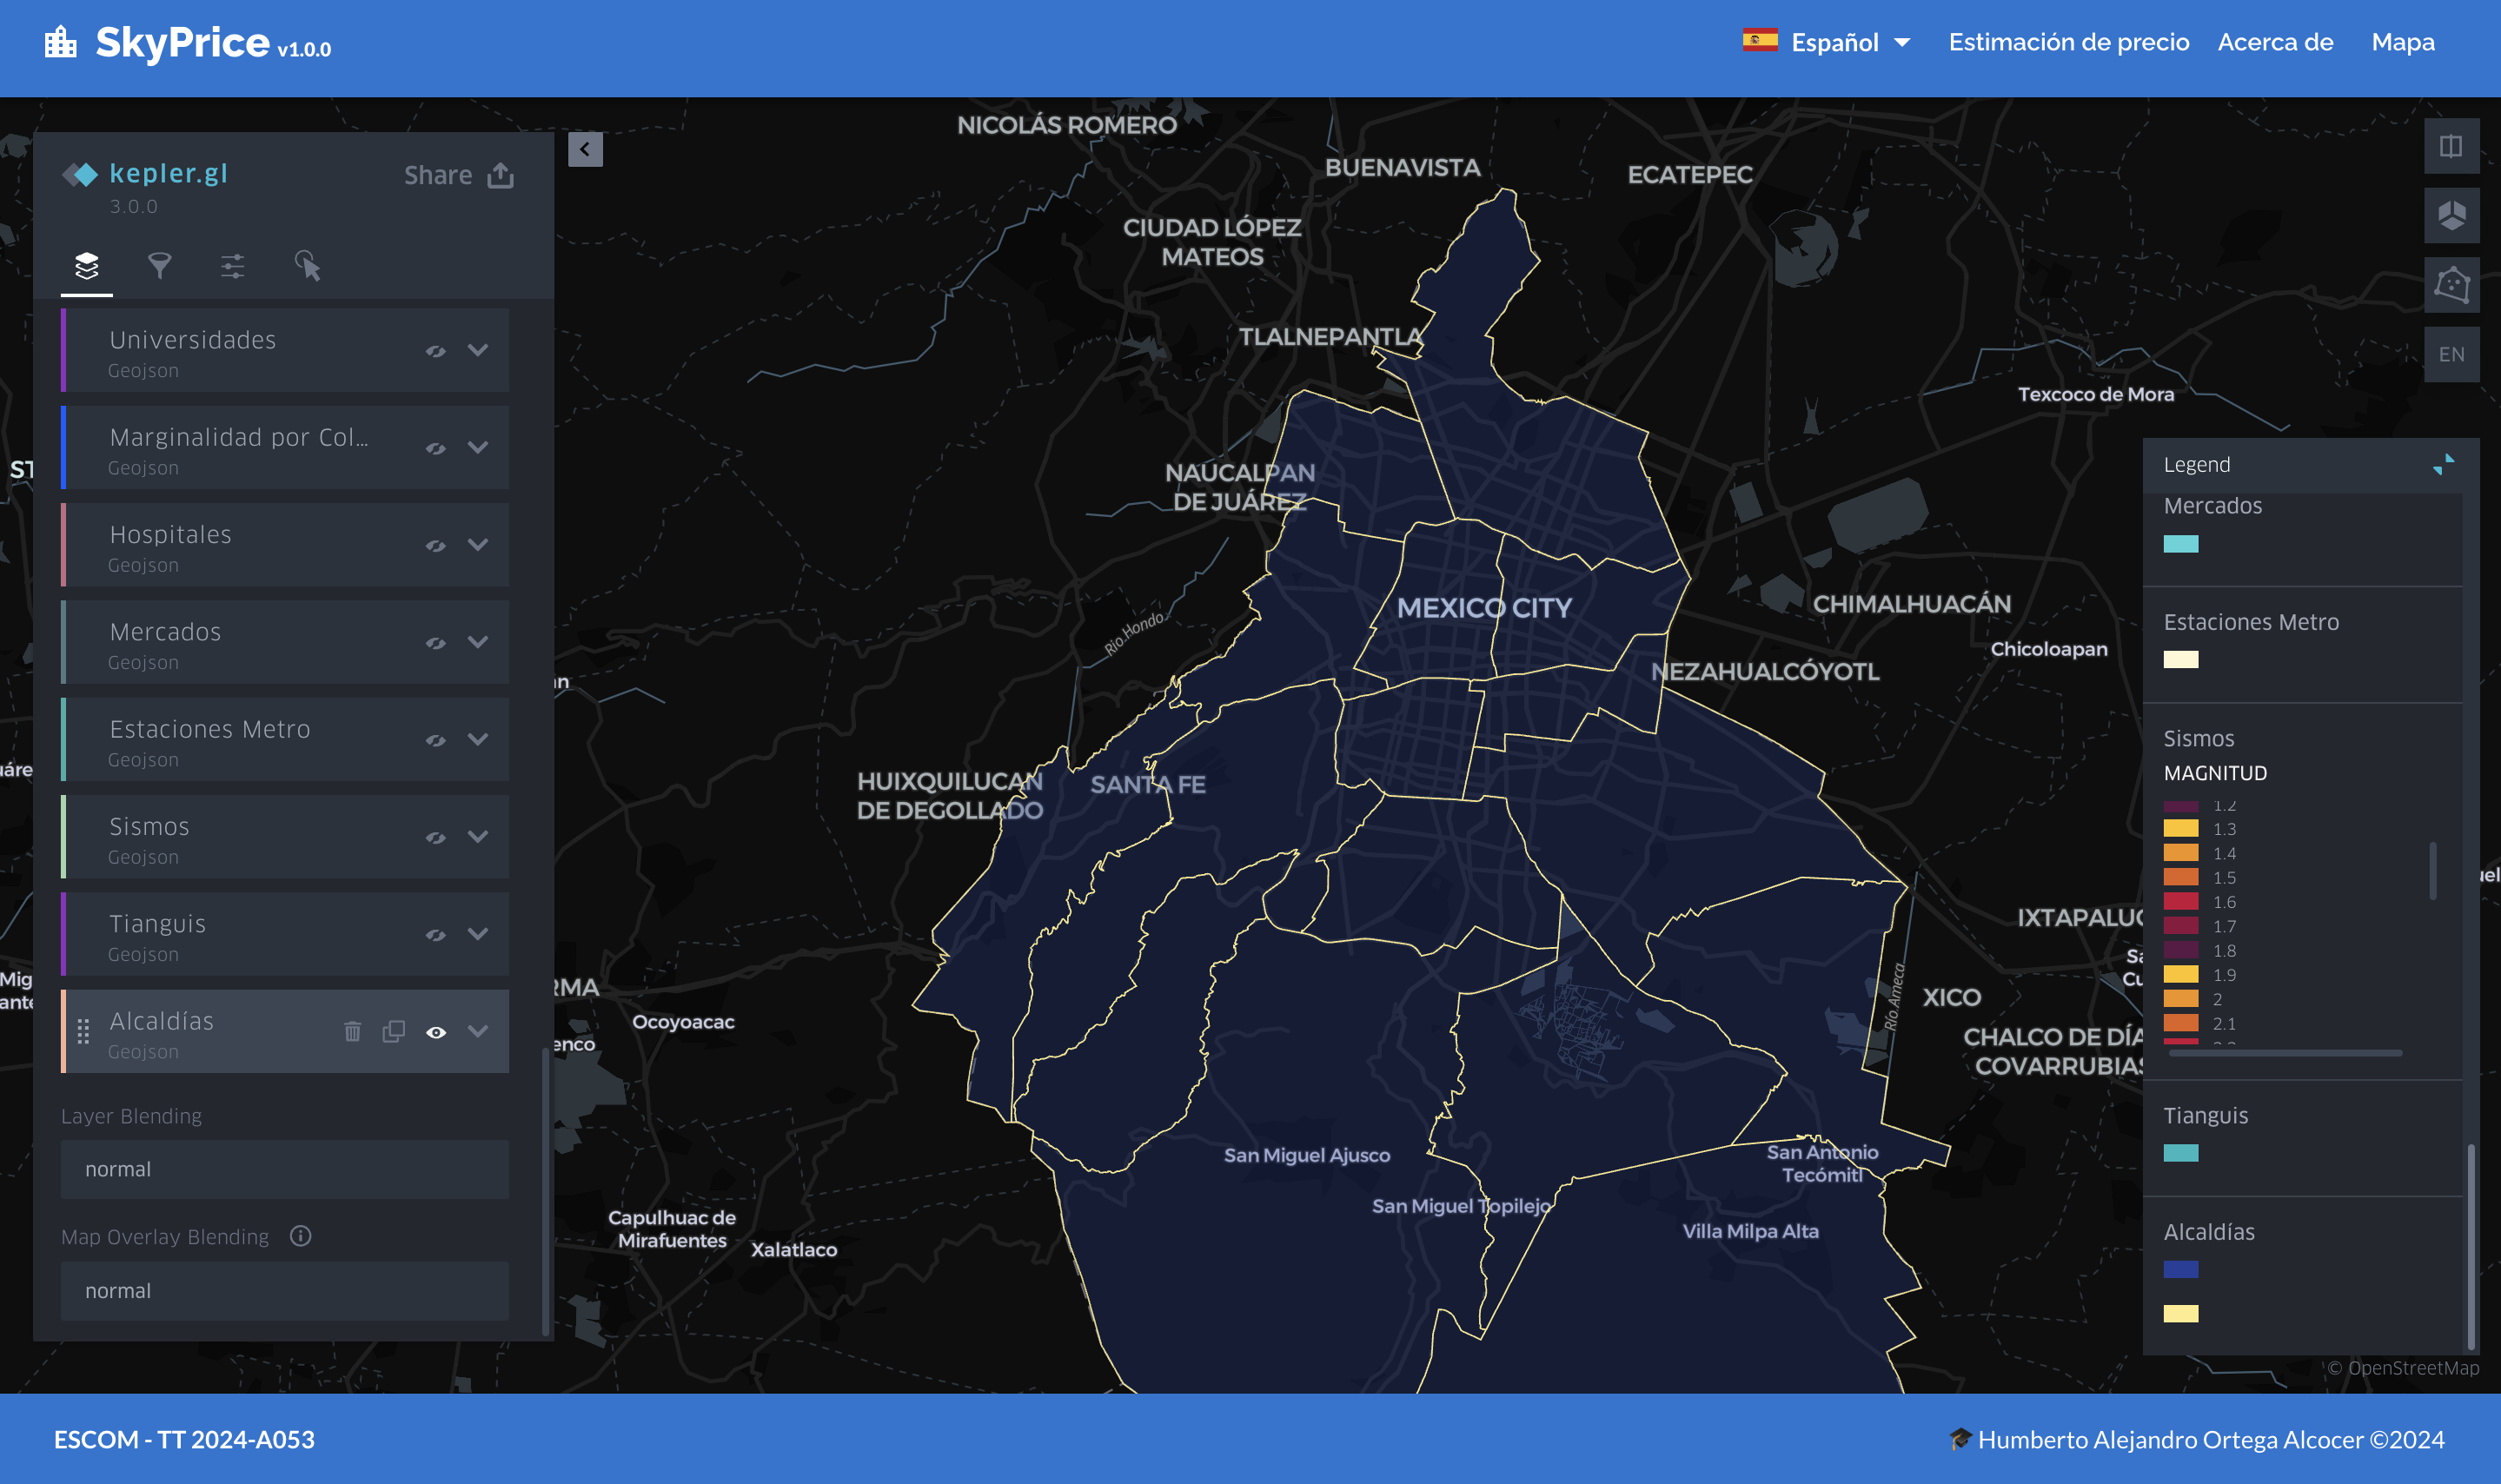
\includegraphics[width=0.8\textwidth]{imagenes/05-mapa-interactivo/alcaldias.png}
    \caption{Alcaldías}
    \label{fig:alcaldias}
\end{figure}


\section{Funcionalidades avanzadas}
La herramienta \textit{kepler.gl} ofrece una amplia gama de funcionalidades
avanzadas que permiten al usuario personalizar la visualización de los datos
geoespaciales. A continuación se describen algunas de las funcionalidades más
importantes.

\subsection{Agregar datos}
Una de las funcionalidades más importantes de \textit{kepler.gl} es la posibilidad
de agregar datos geoespaciales en formato GeoJSON, CSV y Shapefile. Para agregar
datos, en la figura \ref{fig:avanzado-agregar} se muestra la opción de agregar datos.

\begin{figure}[H]
    \centering
    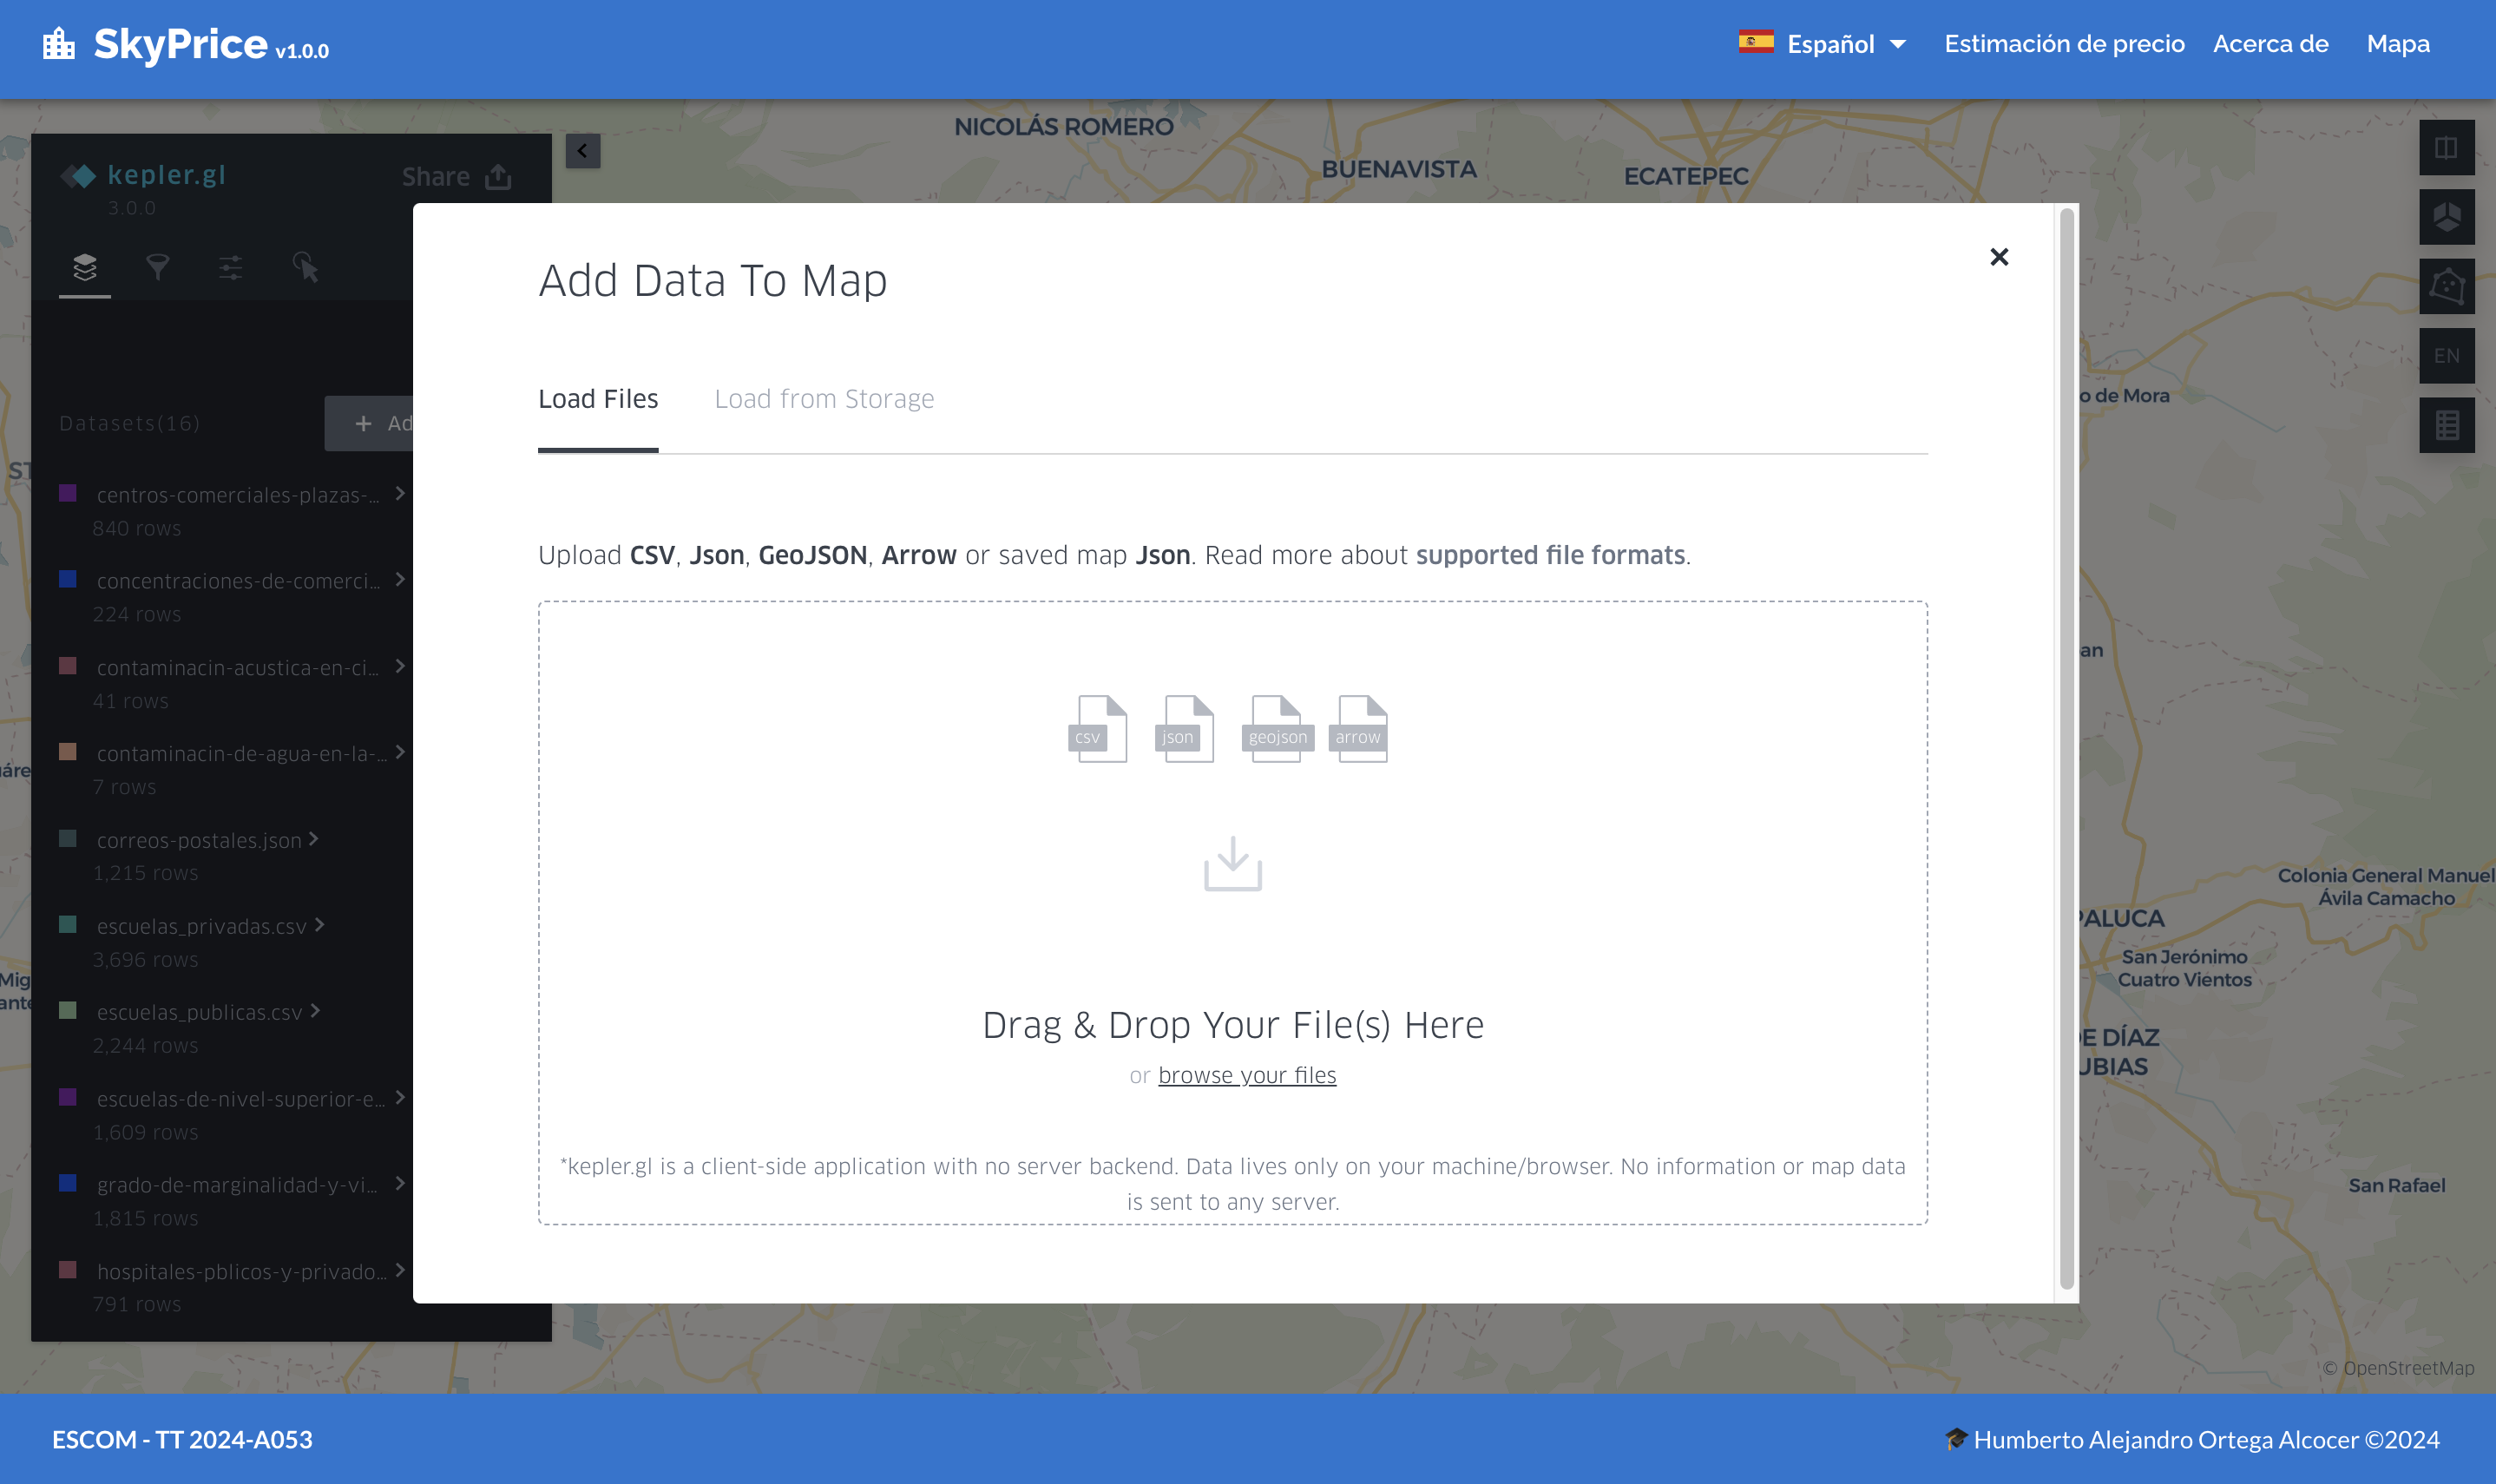
\includegraphics[width=1.0\textwidth]{imagenes/05-mapa-interactivo/avanzado-agregar.png}
    \caption{Agregar datos}
    \label{fig:avanzado-agregar}
\end{figure}

\subsection{Tipos de capas}
Para poder visualizar los datos de forma adecuada, \textit{kepler.gl} ofrece
varios tipos de capas que se pueden utilizar para representar los datos
geoespaciales. Algunos de los tipos de capas más comunes son:

\begin{itemize}
    \item Capa de puntos: se utiliza para representar ubicaciones puntuales en
    el mapa.
    \item Capa de polígonos: se utiliza para representar áreas en el mapa.
    \item Capa de líneas: se utiliza para representar rutas o líneas en el mapa.
    \item Capa de grilla: se utiliza para representar datos agregados en celdas
    de una grilla.
\end{itemize}

Para seleccionar el tipo de capa, en la figura \ref{fig:avanzado-tipo} se muestra
la opción de seleccionar el tipo de capa.

\begin{figure}[H]
    \centering
    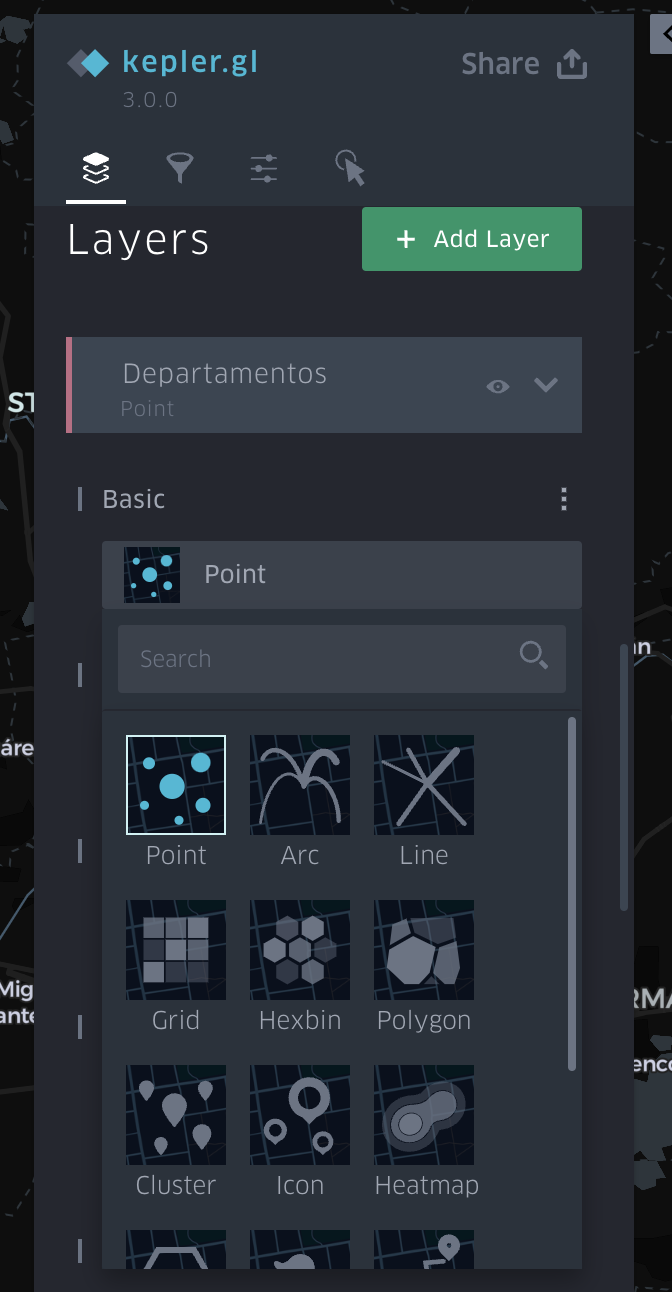
\includegraphics[width=0.3\textwidth]{imagenes/05-mapa-interactivo/avanzado-tipo.png}
    \caption{Selección de tipo de capa}
    \label{fig:avanzado-tipo}
\end{figure}

\subsection{Filtros}
Para poder visualizar los datos de forma más precisa, \textit{kepler.gl} ofrece
la posibilidad de aplicar filtros a los datos geoespaciales. Estos filtros
permiten al usuario seleccionar un subconjunto de los datos que cumplan con
ciertas condiciones. Algunos de los filtros más comunes son:

\begin{itemize}
    \item Filtro por rango: se utiliza para seleccionar los datos que se encuentren
    dentro de un rango específico.
    \item Filtro por categoría: se utiliza para seleccionar los datos que pertenezcan
    a una categoría específica.
    \item Filtro por texto: se utiliza para seleccionar los datos que contengan un
    texto específico.
\end{itemize}

Para aplicar un filtro, en la figura \ref{fig:avanzado-filtro} se muestra la opción
de aplicar un filtro.

\begin{figure}[H]
    \centering
    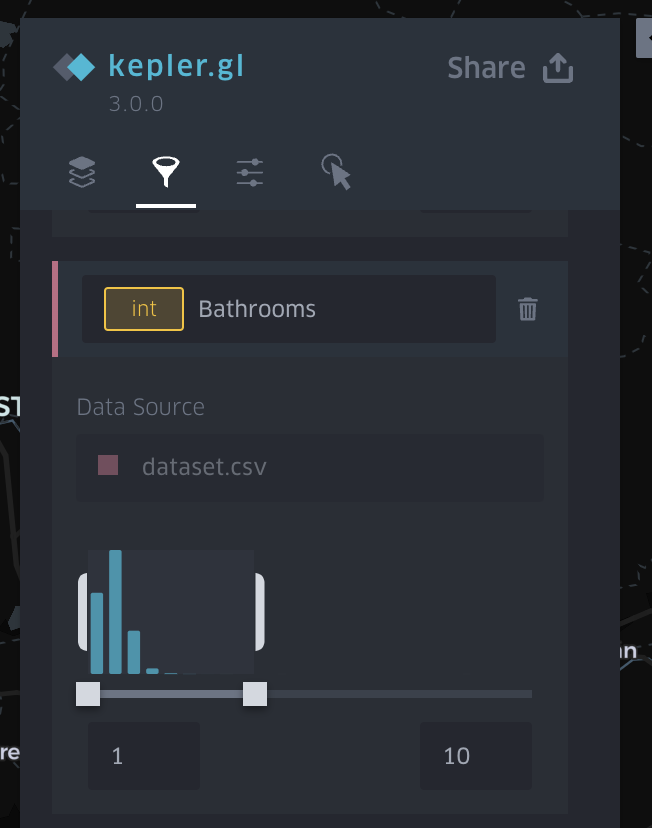
\includegraphics[width=0.3\textwidth]{imagenes/05-mapa-interactivo/avanzado-filtro.png}
    \caption{Aplicación de filtro}
    \label{fig:avanzado-filtro}
\end{figure}

\subsection{Estilos}
Para poder personalizar la visualización de los datos geoespaciales, \textit{kepler.gl}
ofrece la posibilidad de modificar el estilo del mapa. En la figura \ref{fig:avanzado-estilo}
se muestra la opción de modificar el estilo del mapa.

\begin{figure}[H]
    \centering
    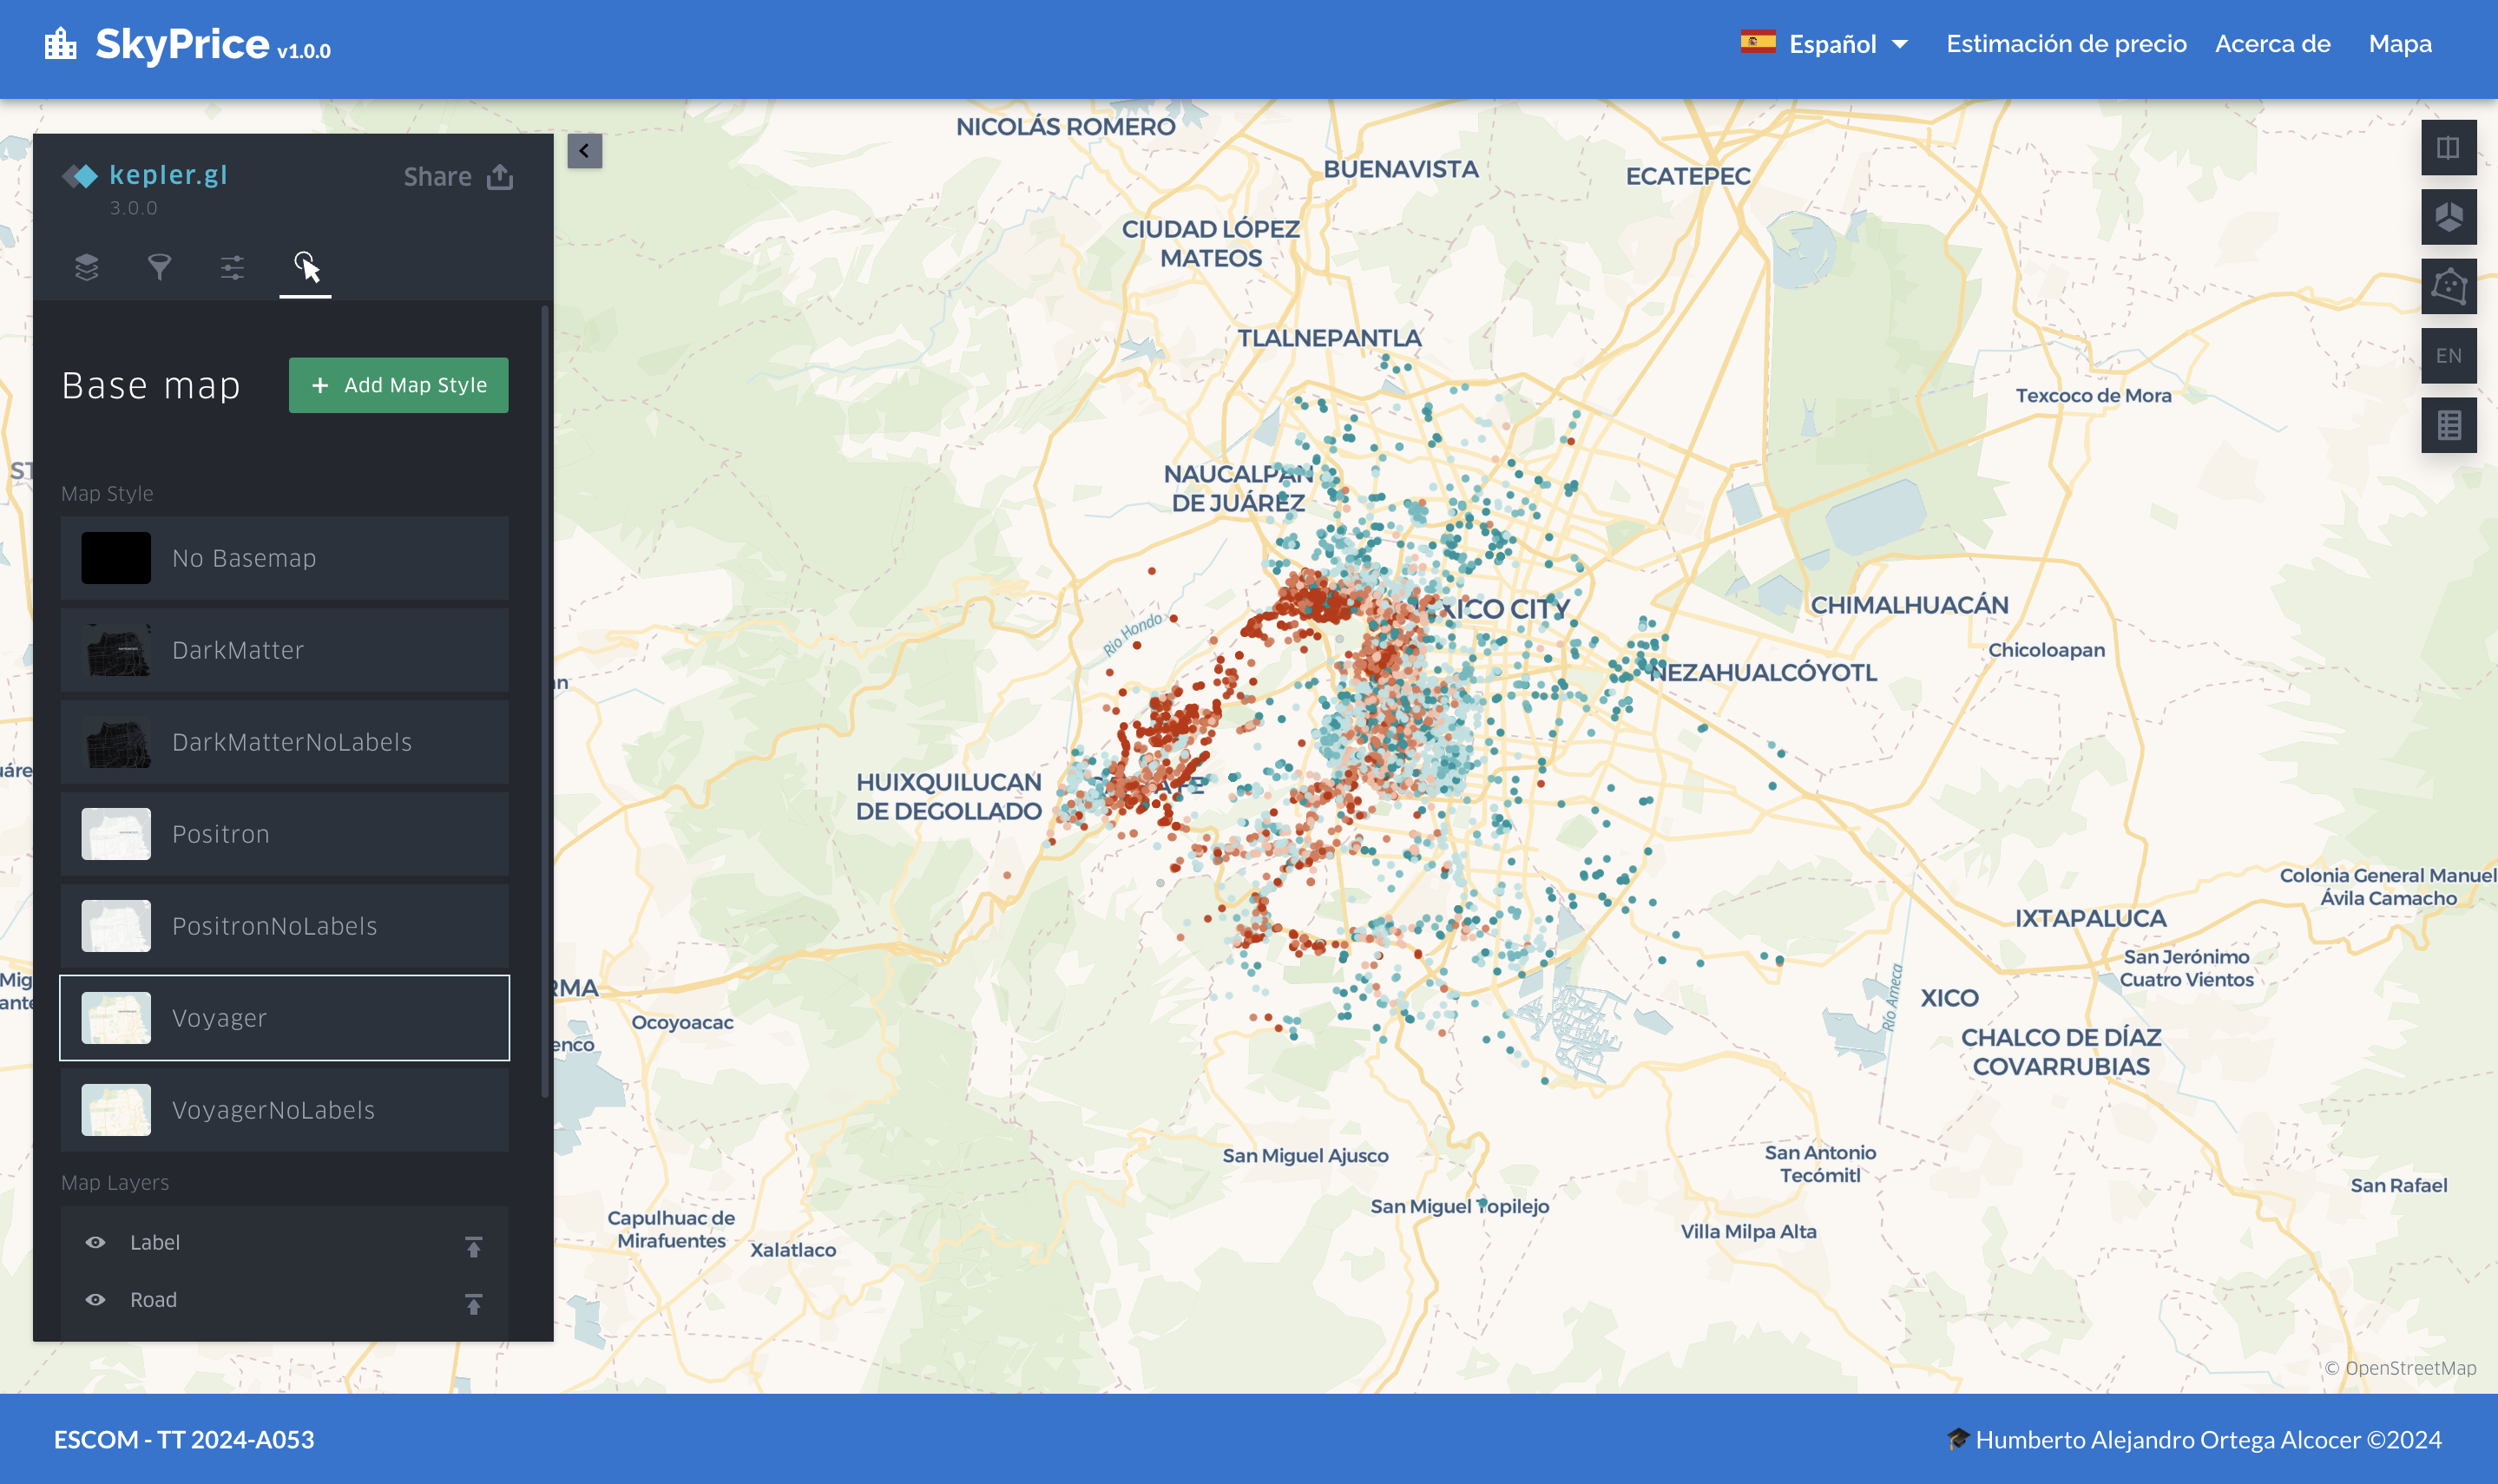
\includegraphics[width=1.0\textwidth]{imagenes/05-mapa-interactivo/avanzado-estilo.png}
    \caption{Modificación de estilo}
    \label{fig:avanzado-estilo}
\end{figure}

\subsection{Exportación}
\textit{kepler.gl} permite exportar los mapas, imágenes y datos geoespaciales
para su uso, manipulación o inspección en otras herramientas. En la figura
\ref{fig:avanzado-exportacion} se muestra la opción de exportar los datos.

\begin{figure}[H]
    \centering
    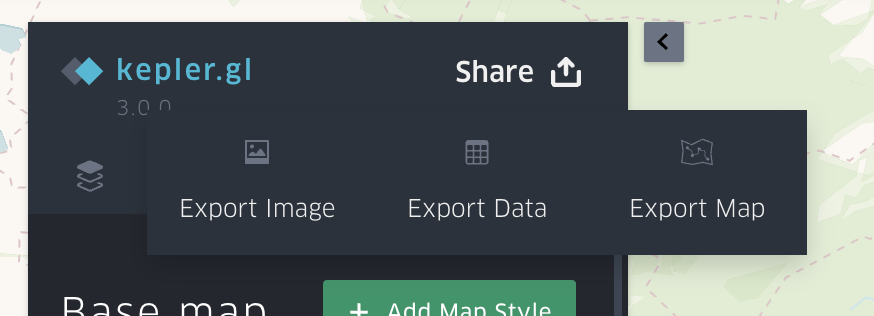
\includegraphics[width=0.8\textwidth]{imagenes/05-mapa-interactivo/avanzado-exportar.png}
    \caption{Exportación de datos}
    \label{fig:avanzado-exportacion}
\end{figure}

\subsubsection{Exportación de imágenes}
\textit{kepler.gl} permite exportar imágenes de los mapas interactivos para su
uso en presentaciones y documentos. En la figura \ref{fig:avanzado-exportacion-imagen}
se muestra la opción de exportar una imagen del mapa interactivo.

\begin{figure}[H]
    \centering
    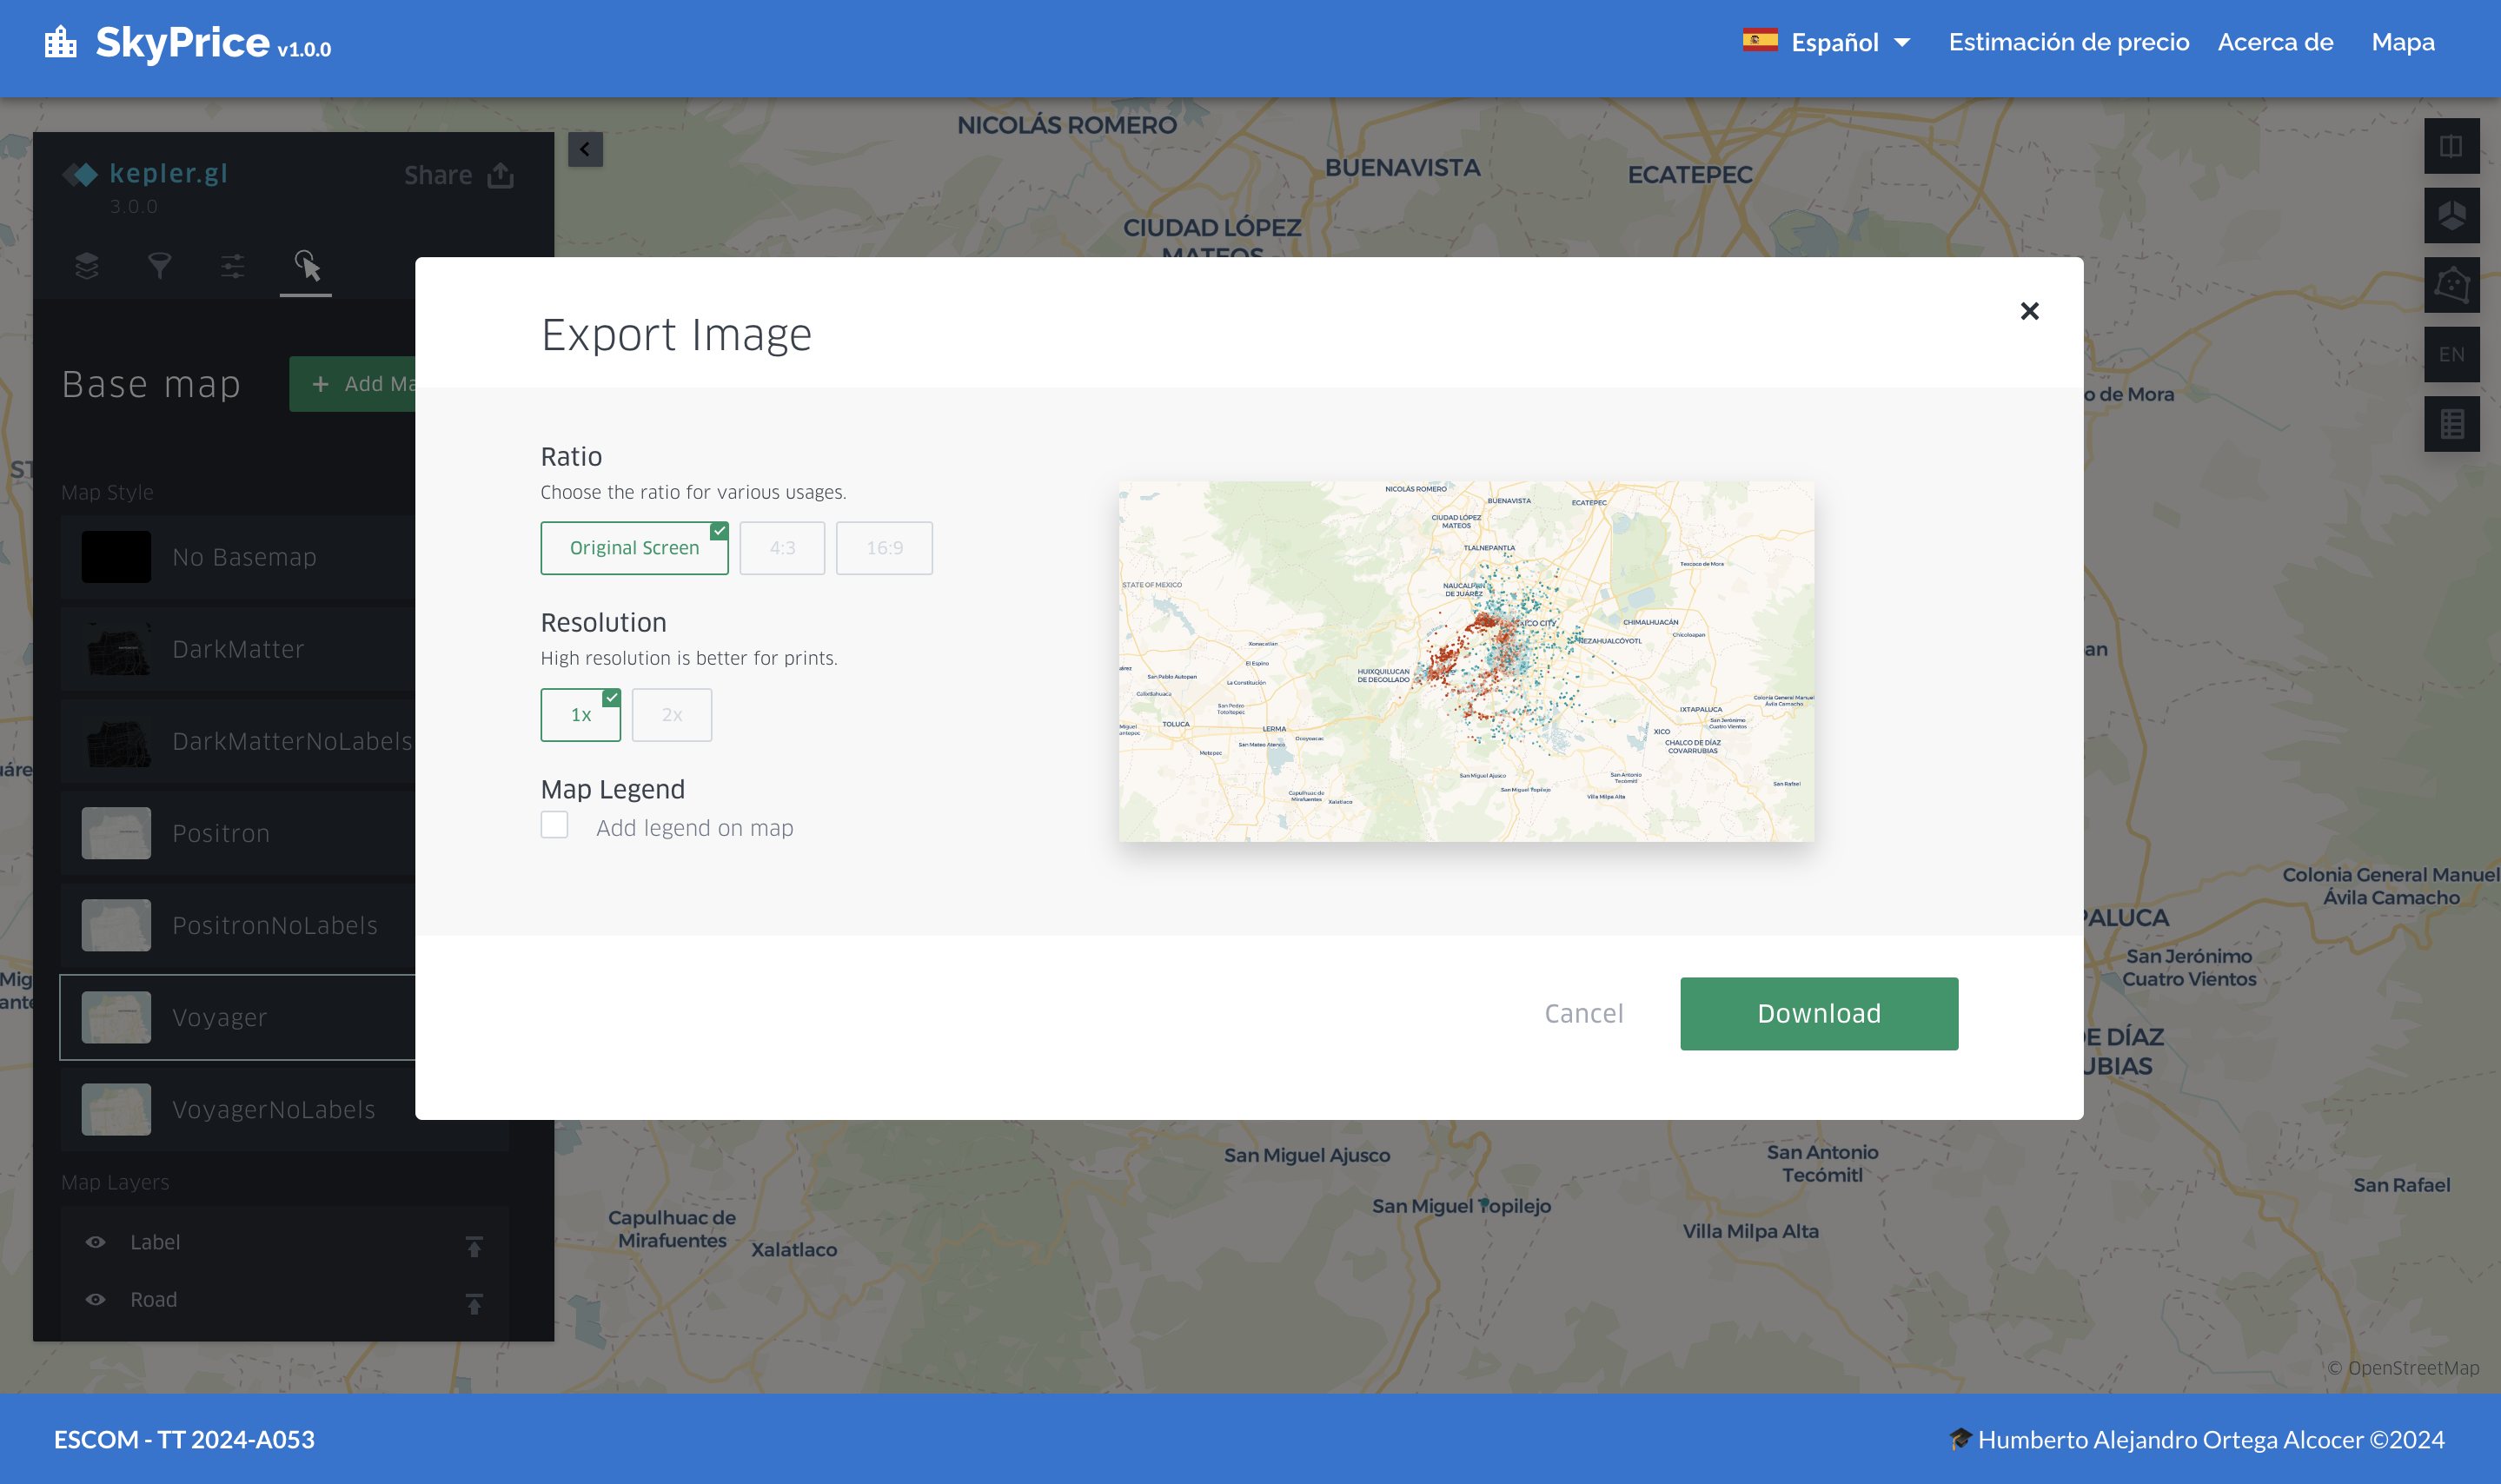
\includegraphics[width=1.0\textwidth]{imagenes/05-mapa-interactivo/avanzado-exportar-imagen.png}
    \caption{Exportación de imagen}
    \label{fig:avanzado-exportacion-imagen}
\end{figure}

\subsubsection{Exportación de mapas}
\textit{kepler.gl} permite exportar los mapas interactivos en formato HTML para
su uso en páginas web. En la figura \ref{fig:avanzado-exportacion-mapa} se muestra
la opción de exportar un mapa interactivo en formato HTML.

\begin{figure}[H]
    \centering
    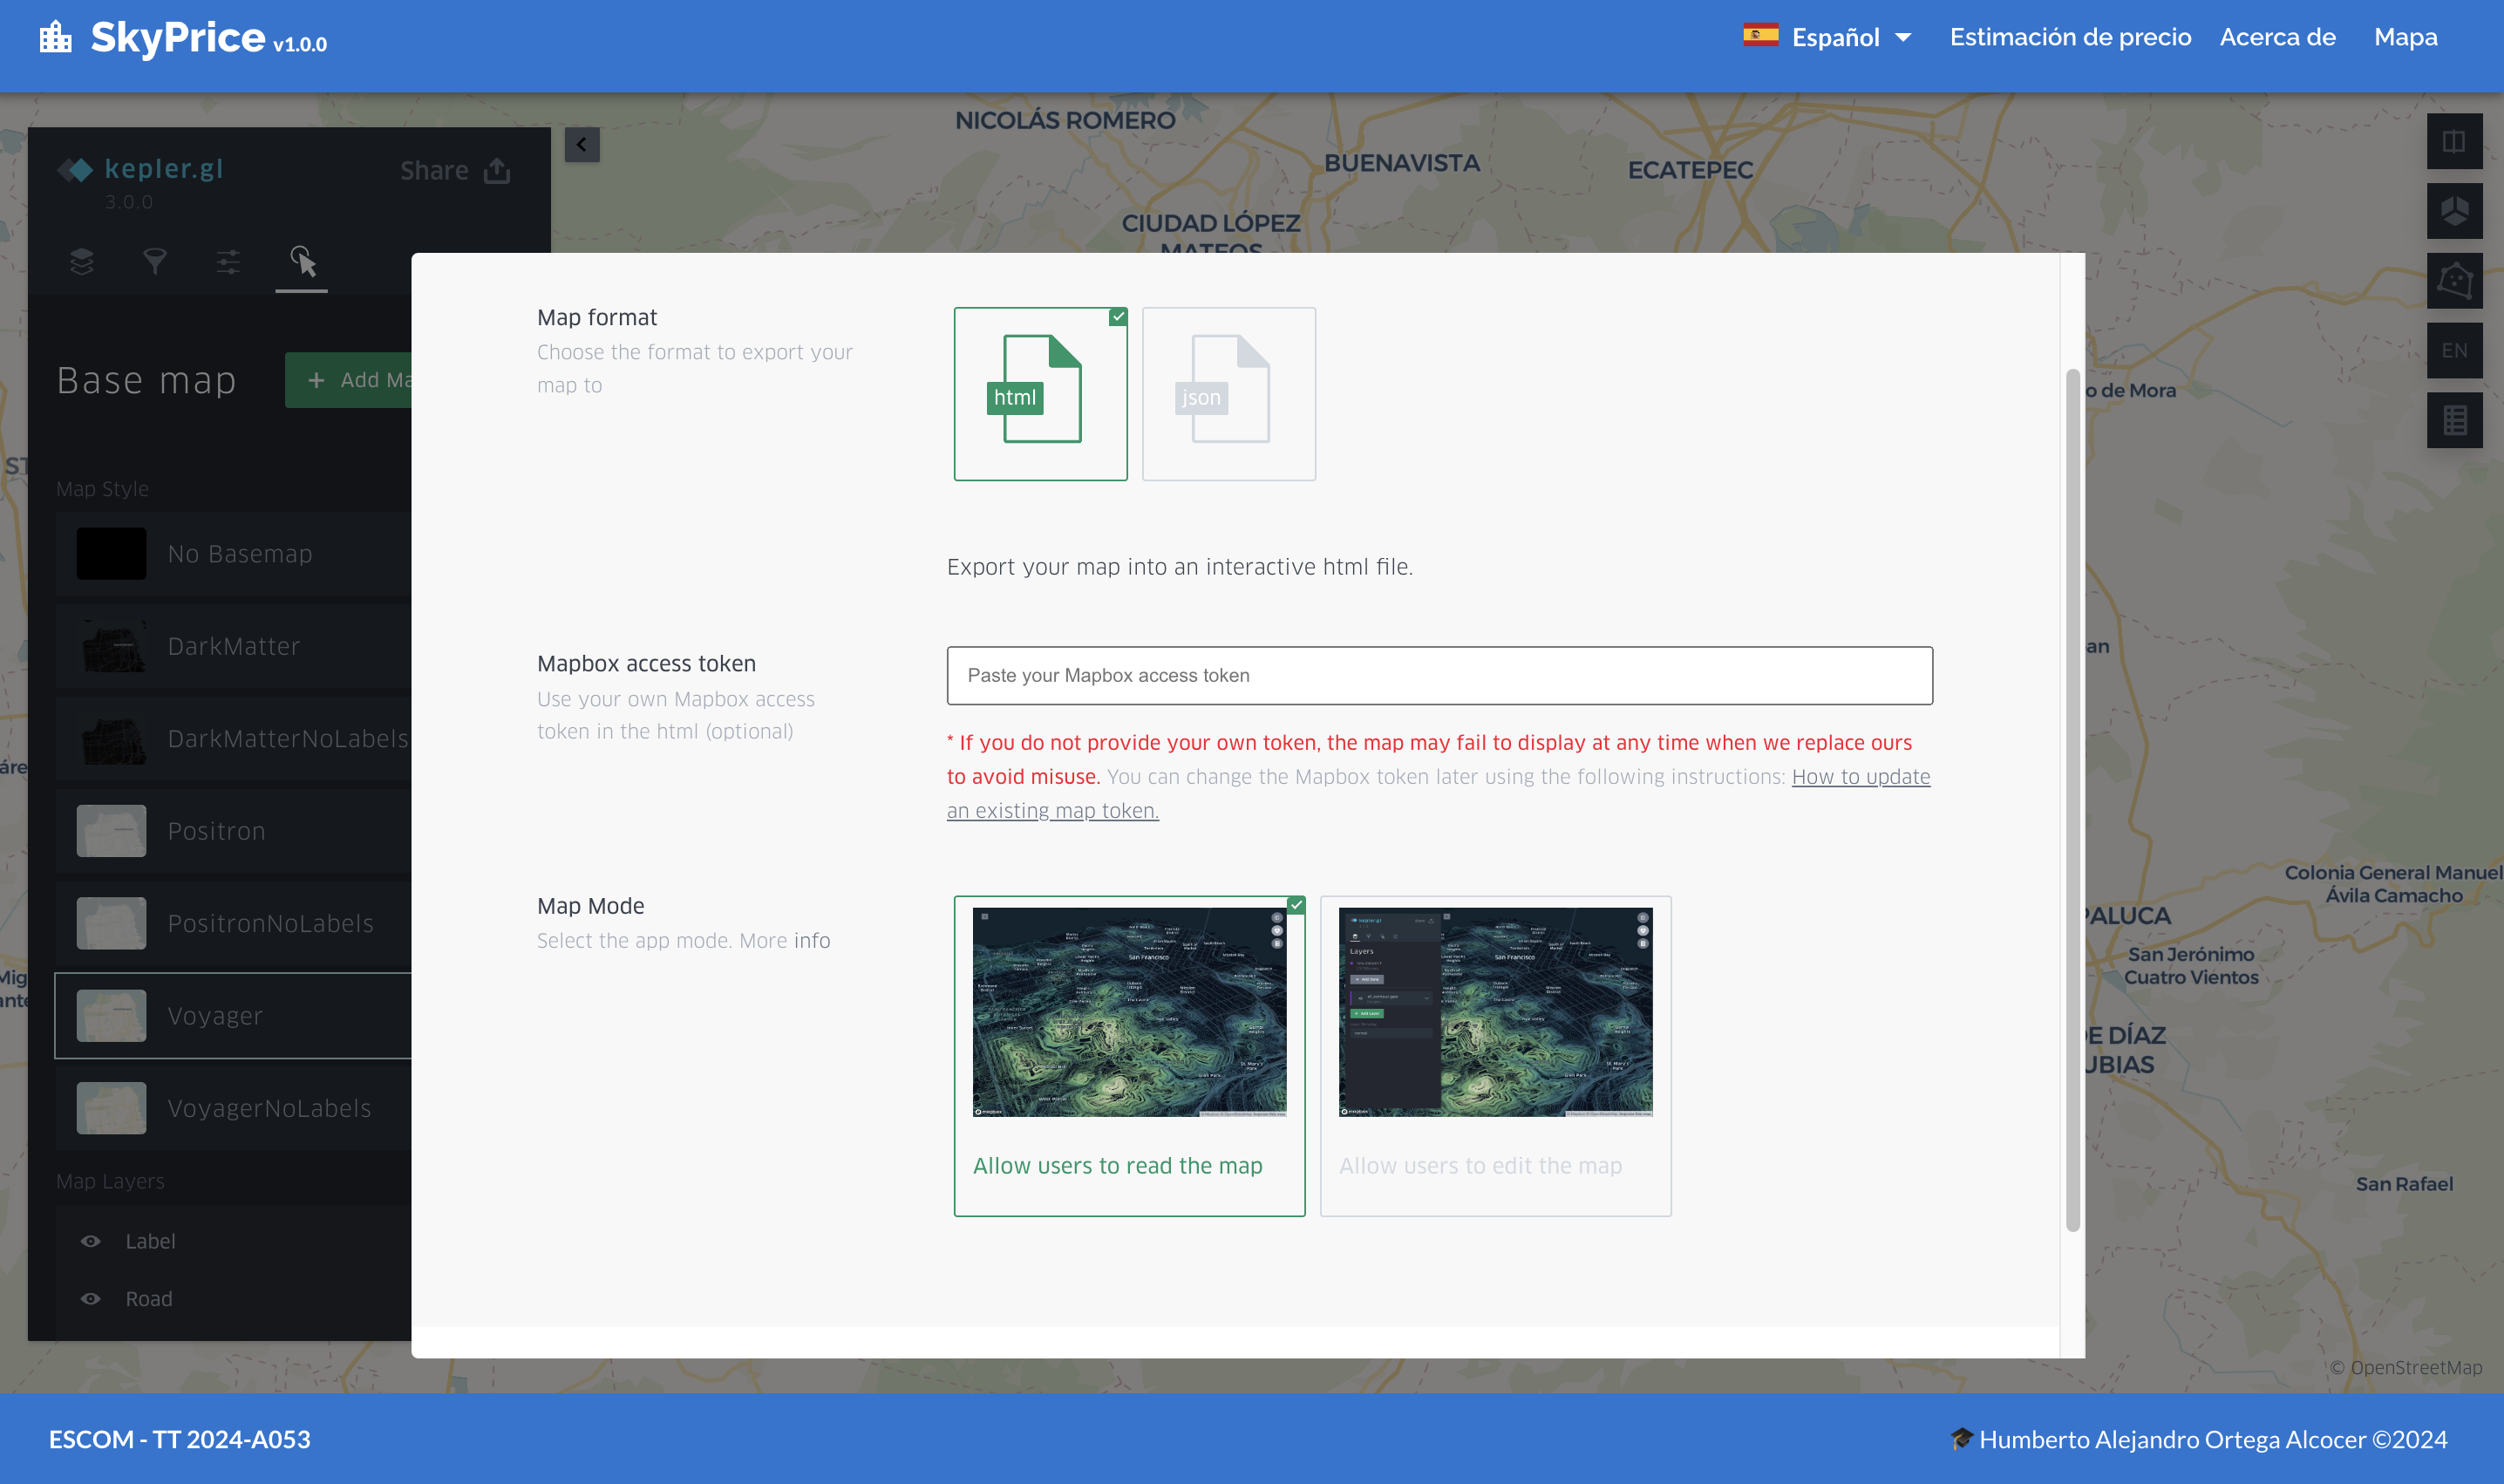
\includegraphics[width=1.0\textwidth]{imagenes/05-mapa-interactivo/avanzado-exportar-mapa.png}
    \caption{Exportación de mapa}
    \label{fig:avanzado-exportacion-mapa}
\end{figure}

\subsubsection{Exportación de datos}
\textit{kepler.gl} permite exportar los datos geoespaciales en formato CSV. Esto
permite al usuario utilizar los datos en otras herramientas de análisis de datos.
En la figura \ref{fig:avanzado-exportacion-datos} se muestra la opción de exportar
los datos geoespaciales en formato CSV.

\begin{figure}[H]
    \centering
    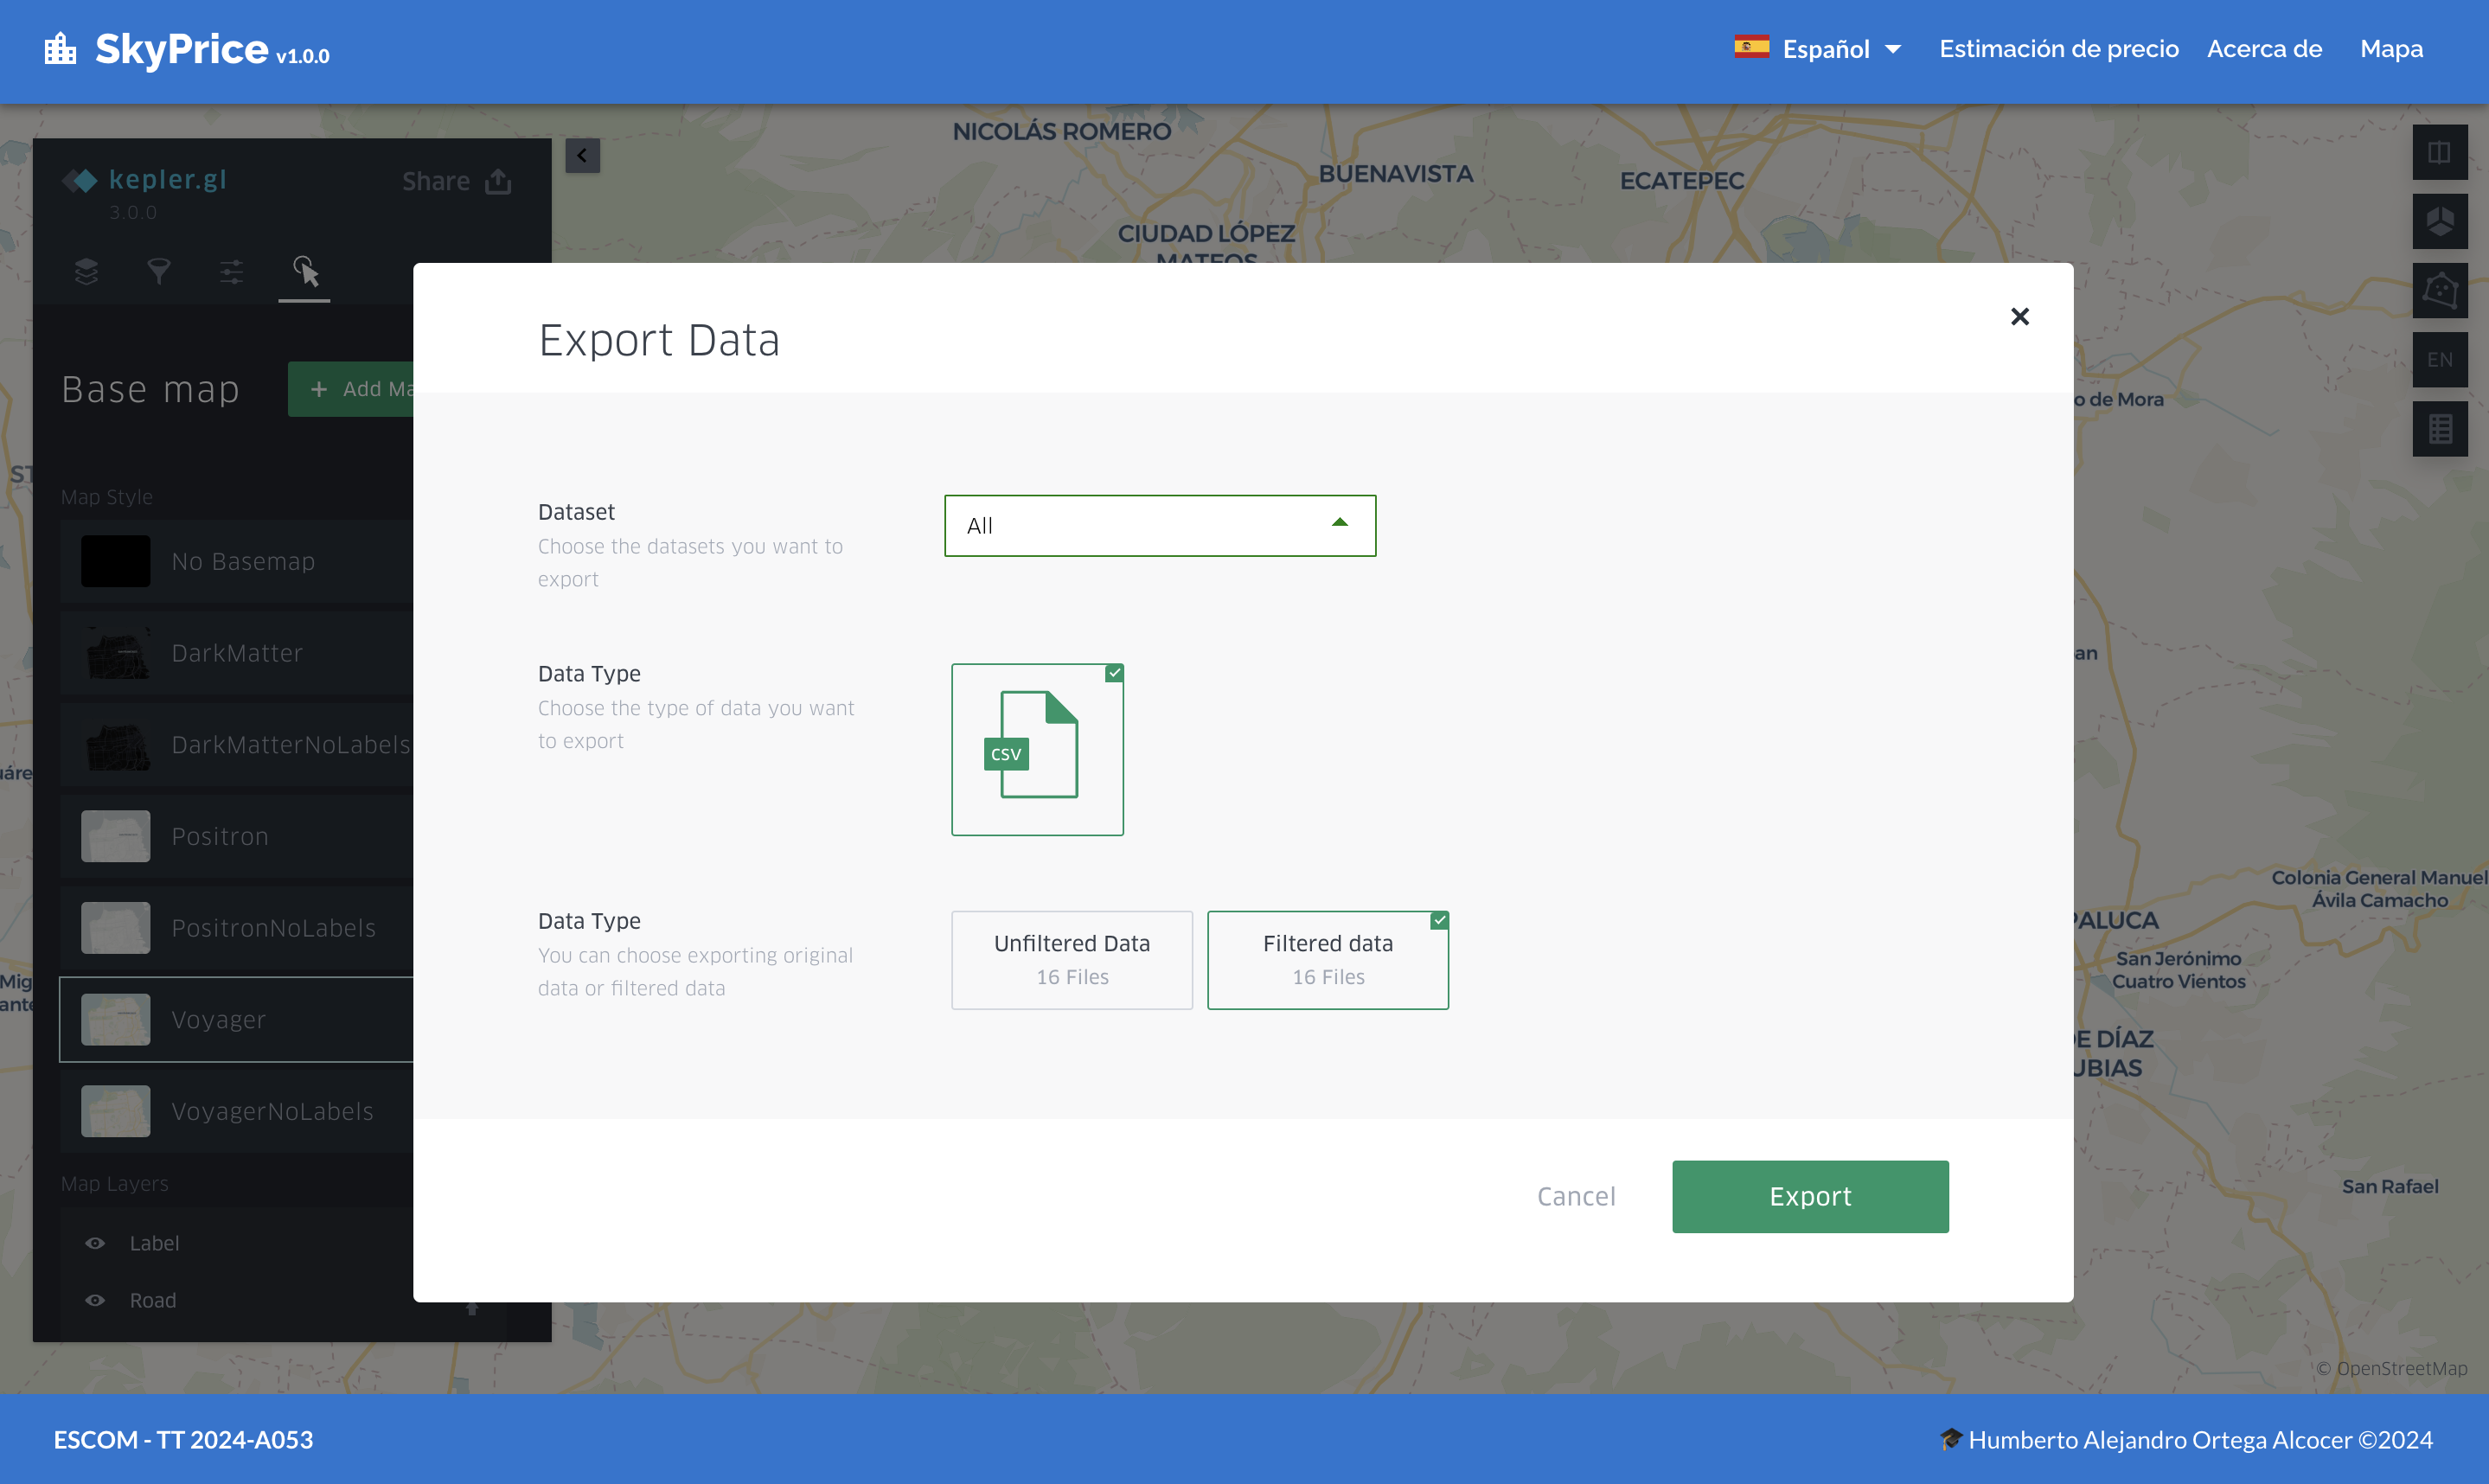
\includegraphics[width=1.0\textwidth]{imagenes/05-mapa-interactivo/avanzado-exportar-datos.png}
    \caption{Exportación de datos}
    \label{fig:avanzado-exportacion-datos}
\end{figure}

